% !TEX TS-program = LuaLaTeX
\documentclass[10pt]{beamer}
\usepackage{pgfpages}
% \setbeameroption{show notes on second screen}

\usetheme[subsectionpage=progressbar]{metropolis}
% \usetheme[]{metropolis}
\usepackage{appendixnumberbeamer}
\usepackage{booktabs}
\usepackage[scale=2]{ccicons}
\usepackage{pgfplots}
\usepgfplotslibrary{dateplot}
\usepackage{xspace}
\newcommand{\themename}{\textbf{\textsc{metropolis}}\xspace}
\usepackage{subcaption}
% \setbeamertemplate{note page}[plain]
\usepackage{media9}
\setbeamertemplate{bibliography item}{\insertbiblabel}

\usepackage{graphicx}
\usepackage[space]{grffile}

\usepackage{makecell}
\usepackage{tikz}
\usetikzlibrary{arrows}
\usepackage{flexisym}
\usepackage[numbers,sort&compress]{natbib}

\title{The Effects of Concurrent Bandwidth Feedback on Robotics Manual Control Tasks}
\subtitle{An Experimental and Modeling Study}
\date{August 29th, 2018}
\author{John Austin Karasinski}
\institute{Qualifying Examination}

\begin{document}

\maketitle

\begin{frame}{Outline}
  \setbeamertemplate{section in toc}[sections numbered]
  \tableofcontents[]
\end{frame}

\section{Introduction}

\begin{frame}[fragile]{About Me}
  \begin{columns}[T]
    \begin{column}{.6\textwidth}
      \begin{description}[align=right]
        \setlength\itemsep{1em}
        \item [2012] B.S. Physics, UCSC\\
              Software Engineer, MV
        \item [2013] Start at UC Davis
        \item [2016] M.S. MAE, UCD\\
              Intern, ARC
        \item [2017] Link Fellowship\\
              Pathways Intern, ARC
      \end{description}
    \end{column}
    \begin{column}{.4\textwidth}
      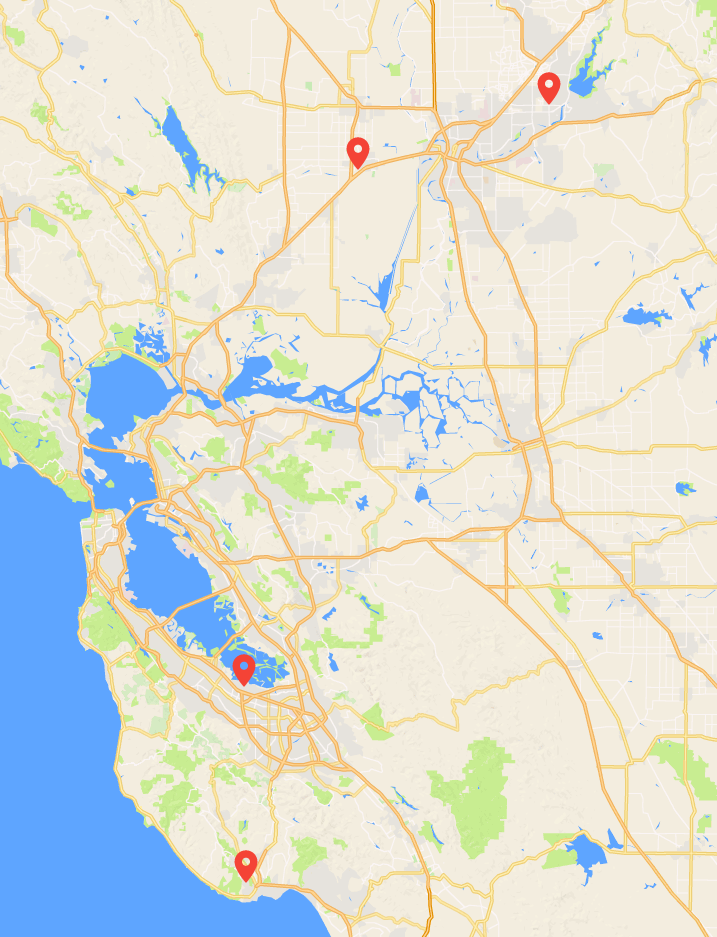
\includegraphics[width=\textwidth]{../img/california.png}
    \end{column}
  \end{columns}
\end{frame}

\begin{frame}[fragile]{Goal}
  Measure, model, and predict the effects of concurrent bandwidth feedback (CBF) on human performance in robotics manual control tasks.
\end{frame}

\section{Research Aims}

\begin{frame}[fragile]{Research Aims}
  \begin{description}[align=right]
    \setlength\itemsep{1em}
    \item [Aim One] Feedback effects in a three-axis manual tracking task
    \item [Aim Two] Feedback effects in a robotics track and capture task
    \item [Aim Three] Extend Structural Model to include feedback effects
  \end{description}
\end{frame}

\section{Background}

\begin{frame}[fragile]{What is feedback?}
  \begin{columns}[T]
    \begin{column}{.8\textwidth}
      \begin{block}{}
        ``Feedback is information about the gap between\\ the actual level and the reference level of a system parameter which is used to alter the gap in some way.'' - Ramaprasad~\cite{Ramaprasad1983}
      \end{block}
    \end{column}
  \end{columns}
  % Feedback can be broadly classified into two types: intrinsic, feedback which is generated from within the context of the action itself, and extrinsic, feedback which is given from an external source~\cite{laurillard1993rethinking}.
\end{frame}

% \begin{frame}[fragile]{Extrinsic Feedback}
%   Extrinsic feedback, which is also known as augmented feedback, has been extensively studied in the field motor learning~\cite{Sigrist2013}.
%   In their 2013 review, Sigrist et al. write ``[i]t is generally accepted that augmented feedback, provided by a human expert or a technical display, effectively enhances motor learning~\cite{Sigrist2013}.''
%   There are a variety of different forms of augmented feedback, that can be further classified by how, when, and by what form the feedback is provided.
%   For this work, however, we sought to evaluate a type of feedback which was both conceptually simple and could be tied to operational requirements.
%   With these requirements in mind, we will investigate the effects of concurrent bandwidth feedback.
%   Concurrent, or real-time, feedback is displayed to the operator while the task is being executed, in contrast to terminal feedback, which is displayed after the task is complete.
%   Bandwidth feedback is displayed to the operator when some parameter is inside (on-track feedback) or outside (off-track feedback) of an acceptable, predefined tolerance limit.
%   In our implementation, concurrent bandwidth feedback describes feedback conveyed to the operator when their real-time performance drifts outside of an acceptable tolerance limit.
% \end{frame}

\begin{frame}[fragile]{Thorndike, 1927~\cite{thorndike1927law}}
  \begin{columns}[T]
    \begin{column}{.6\textwidth}
      \begin{itemize}
        \setlength\itemsep{1em}
        \item Blindfolded line-drawing experiment
        \item Two groups of subjects:\\ \quad With, without bandwidth feedback
        \item Bandwidth feedback resulted\\ in better performance, but was\\ lost in retention
        \item Results consistent with\\ guidance hypothesis
      \end{itemize}
    \end{column}
    \begin{column}{.4\textwidth}
      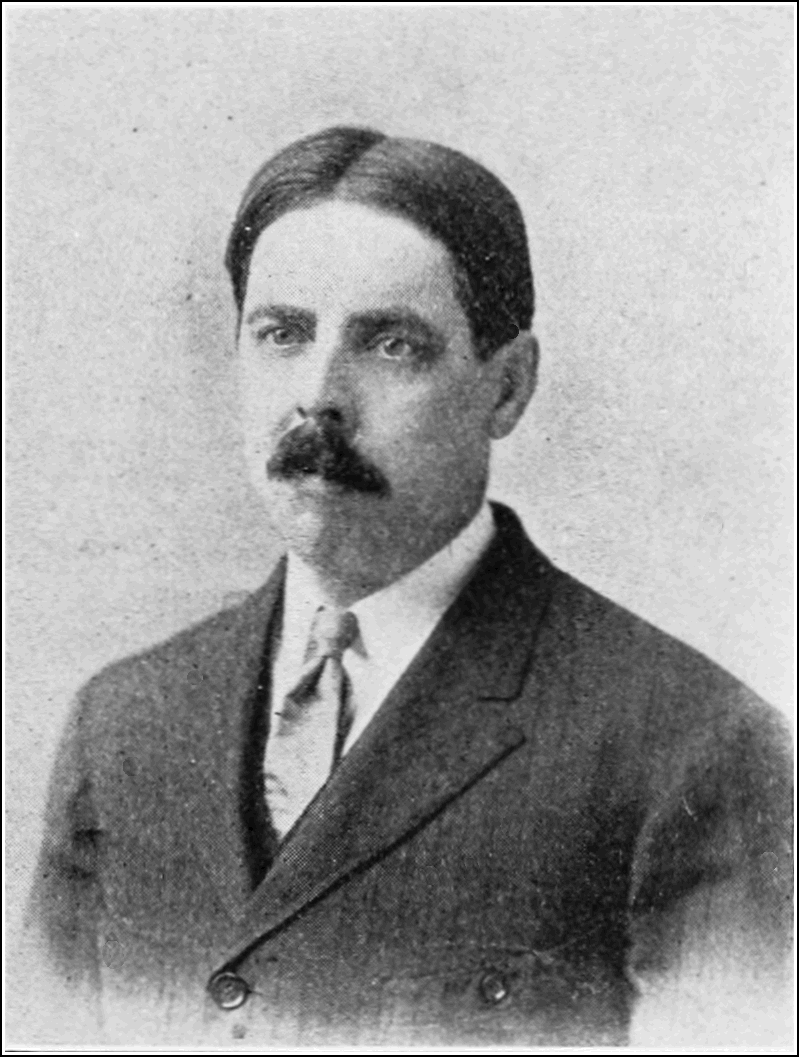
\includegraphics[width=\textwidth]{../img/thorndike.png}
    \end{column}
  \end{columns}
\end{frame}

\begin{frame}[fragile]{Guidance Hypothesis}
  \metroset{block=fill}
  \begin{columns}[T]
    \begin{column}{.8\textwidth}
      % Consistent feedback during the acquisition phase of learning leads to a dependency on the feedback.
      If consistent feedback during the acquisition phase of learning is provided, ``the subject comes to rely on that source of error information to maintain performance, and thus does not deal effectively with the other cues in the task that are important''.\\
      -Salmoni et al., 1984~\cite{salmoni1984knowledge}
    \end{column}
  \end{columns}
\end{frame}

\note[itemize]{
  \item How do we defeat the guidance hypothesis?
  \item Provide feedback which is complementary to other available information, but sufficient in itself to complete the task
  \item Feedback should also fade with time as the subjects perform better
}

\begin{frame}[fragile]{Payne and Hauty, 1955~\cite{payne1955effect}}
  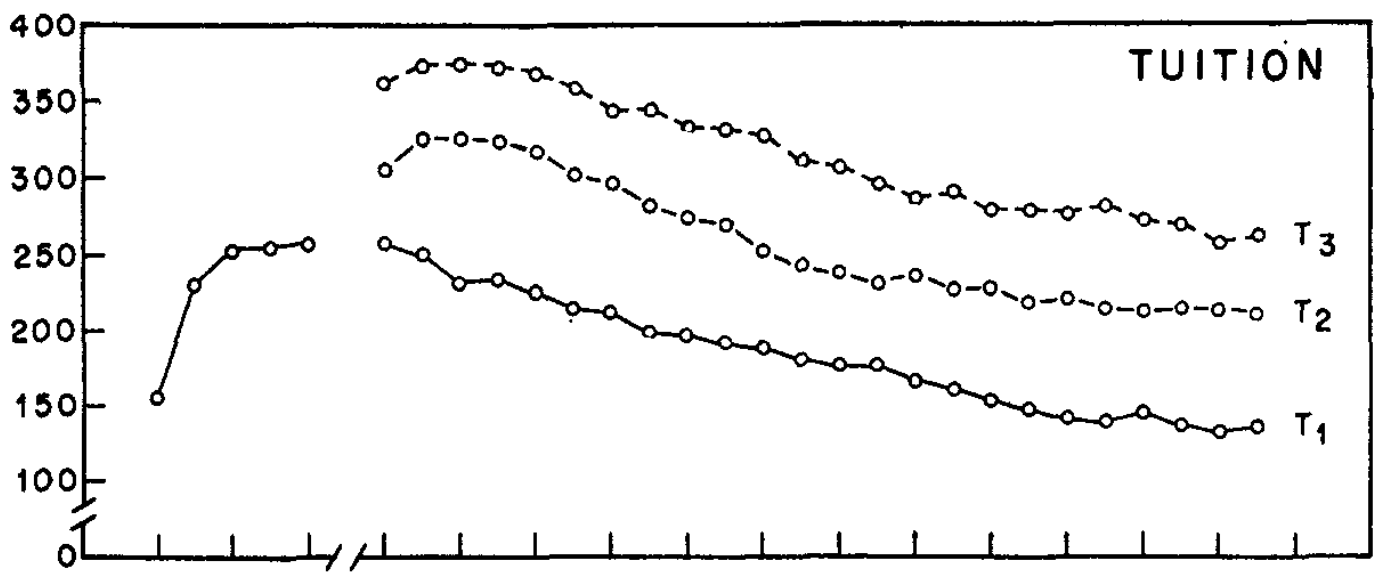
\includegraphics[width=\textwidth]{../img/payneandhauty.png} \\
  \hspace{3em} Training \hspace{1em} Start\hfill 4 hours
\end{frame}

\note[itemize]{
  \item Subjects were placed into one of three feedback groups
  \item a control level, where no feedback was provided
  \item a second level, which included a single peripheral visual signal when a deviation in one of the displays occurred, but did not specify which instrument
  \item a third level, which provided individual indicators for each of the four instruments, and noted the locus of the deviation.
  \item They concluded by stating that ``the increment is a positive function of the specificity of the information supplied, it can be ascribed largely to the directive properties of the cues, i.e., the cues impose a more efficient temporal and spatial organization upon [the subject's] scanning behavior~\cite{payne1955effect}.''
}

\begin{frame}[fragile]{Gordon and Gottlieb, 1967~\cite{Gordon1967}}
  \begin{center}
    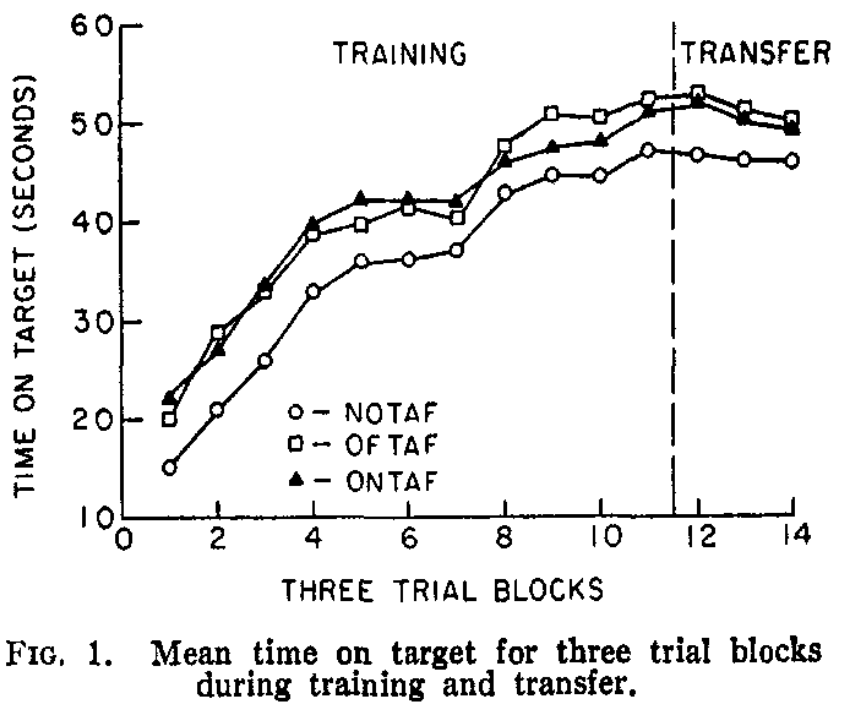
\includegraphics[width=0.8\textwidth]{../img/gordonandgottlieb.png}
  \end{center}
\end{frame}

\note[itemize]{
  \item Subjects were placed into one of three feedback groups
  \item Control and off-track and on-track feedback groups
  \item Both treatment groups performed better than control, even during retention when feedback was removed
}

\begin{frame}[fragile]{de Groot et al., 2011~\cite{DeGroot2011}}
  \begin{center}
    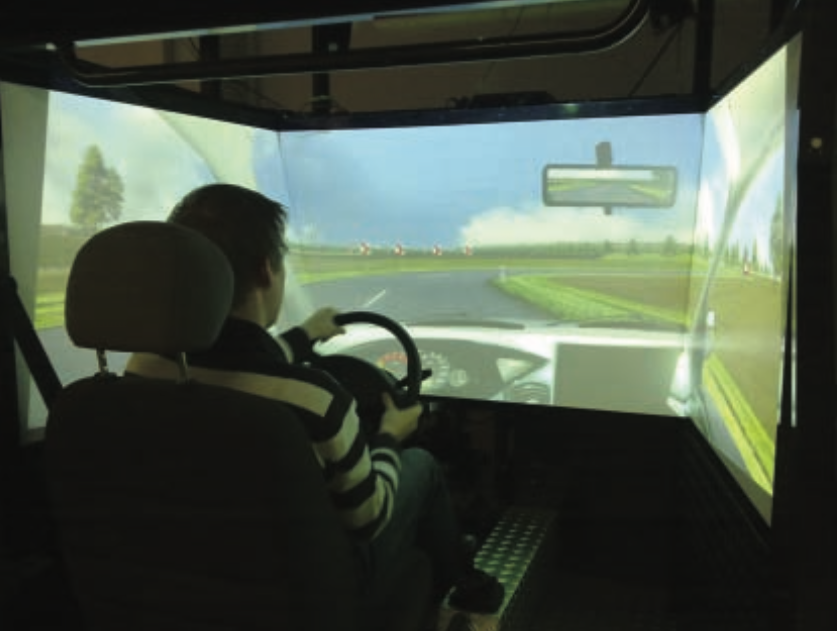
\includegraphics[width=0.8\textwidth]{../img/degrootdriving.png}
  \end{center}
\end{frame}

\begin{frame}[fragile]{de Groot et al., 2011~\cite{DeGroot2011}}
  \begin{center}
    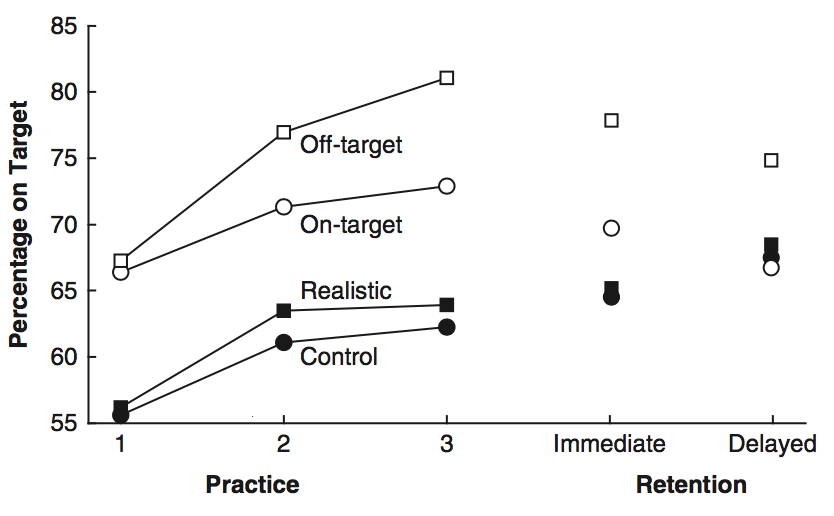
\includegraphics[width=\textwidth]{../img/degrootresults.png}
  \end{center}
\end{frame}

\note[itemize]{
  \item investigated the effects of on-track and off-track feedback compared to a control group
  \item Instead of using a visual indicator, used haptic feedback in the form of a vibrating chair
  \item Retention trials, showed majority of improvement lost during when the feedback was removed
  \item The off-target group, though, did still retain some minor performance improvement, onset advantage~\cite{fischer2008differential}.
  \item ``suggests that the sudden onset of a stimulus is a more powerful perceptual event than a stimulus offset, facilitating low-level perceptual processing and resulting in faster reaction times~\cite{DeGroot2011}.''
}

\begin{frame}[fragile]{SAFER Experiment}
  \begin{itemize}
    \setlength\itemsep{1em}
    \item We investigated feedback strategies in my Masters thesis
    \item Simplified Aid for EVA Rescue (SAFER)
    \item 4 degree of freedom task with two-choice secondary task
  \end{itemize}
\end{frame}

\begin{frame}[fragile]{SAFER}
  \begin{columns}[T]
    \begin{column}{.5\textwidth}
      \hfill
      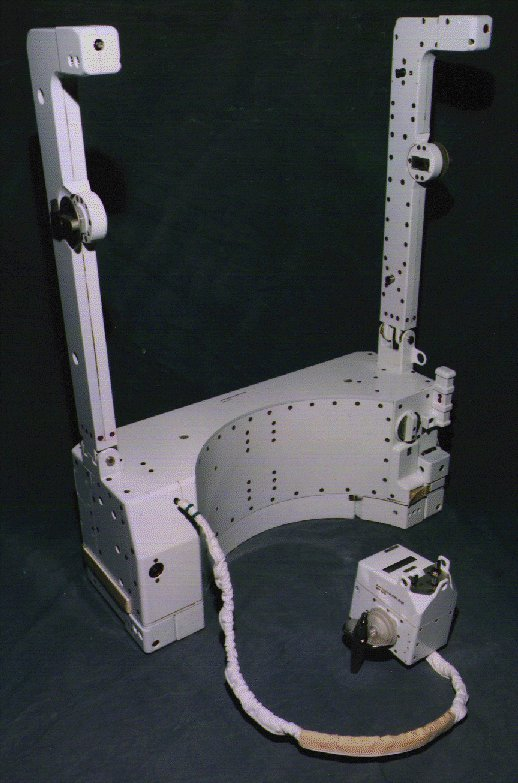
\includegraphics[height=1.3\textwidth]{../img/SAFER_-_Simplified_Aid_for_EVA_Rescue_2.jpg}
    \end{column}%
    \begin{column}{.5\textwidth}
      \includegraphics[width=1.3\textwidth,angle=-90]{../img/SAFER_-_Simplified_Aid_for_EVA_Rescue.jpg}
    \end{column}
  \end{columns}
\end{frame}

\begin{frame}[fragile]{International Space Station}
  \begin{figure} \centering
    \begin{tikzpicture}[
        every node/.style={anchor=south west,inner sep=0pt},
        x=1mm, y=1mm,
      ]
      \only<1-> \node (fig1) at (0,0)
      {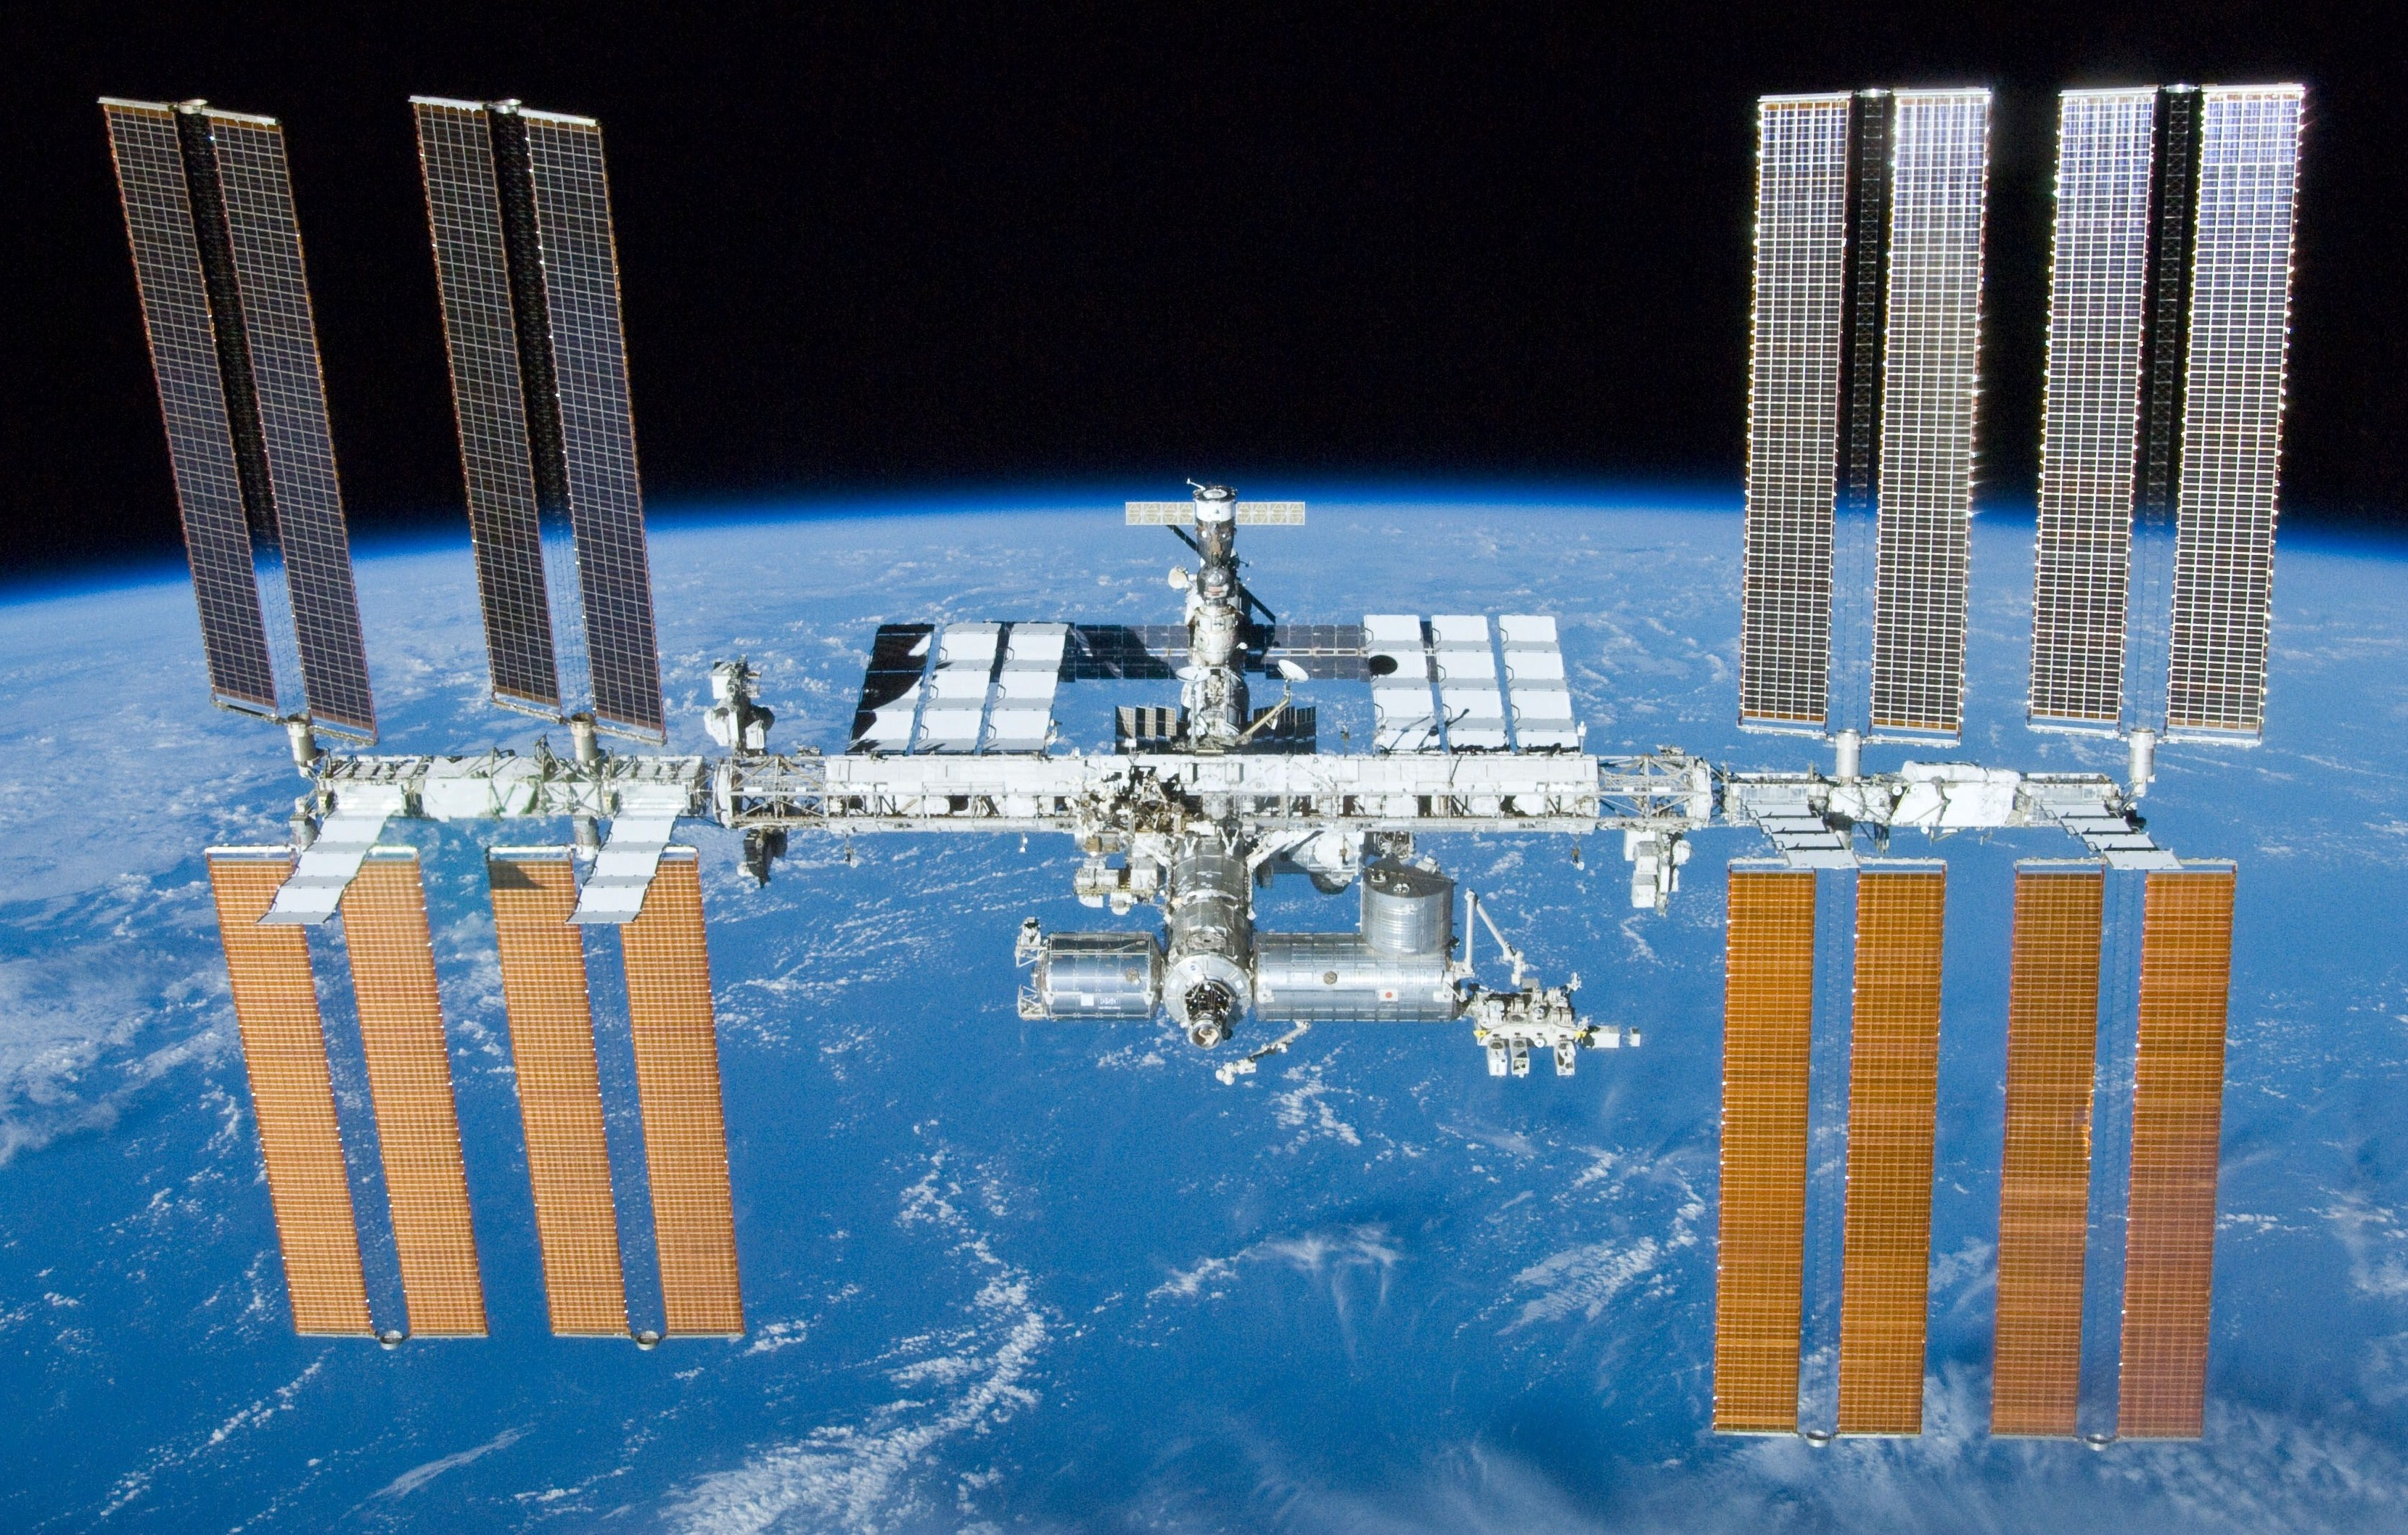
\includegraphics[scale=0.3]{../img/International_Space_Station_after_undocking_of_STS-132.jpg}};
      \only<2->{\node (fig2) at (3,3)
      {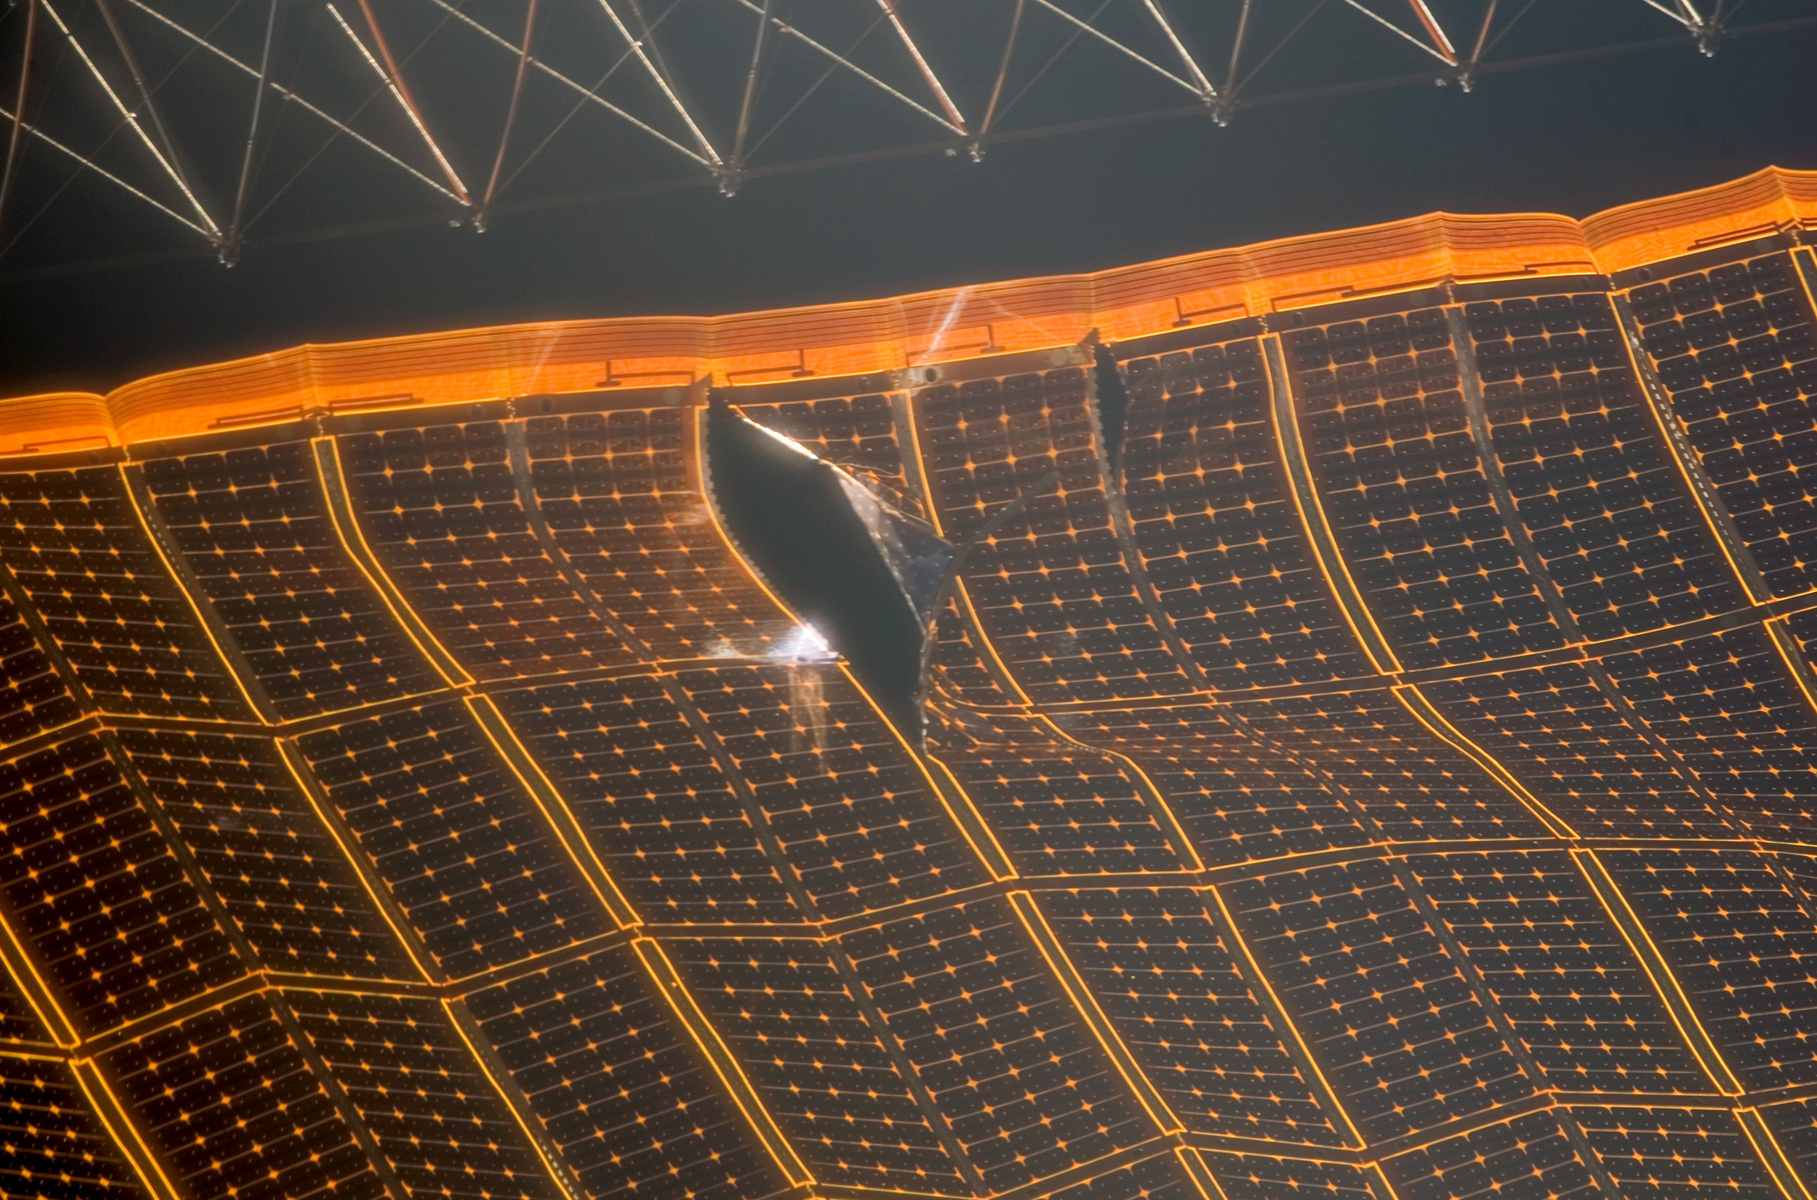
\includegraphics[scale=0.08]{../img/STS120SolarPanel.jpg}};}
      \only<3->{\node (fig2) at (70,2.8)
      {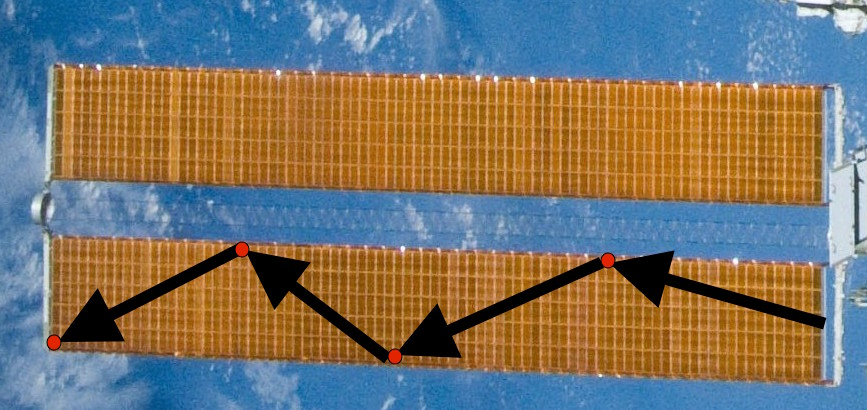
\includegraphics[scale=0.3,angle=90]{../img/waypoints.jpeg}};}
    \end{tikzpicture}
  \end{figure}
\end{frame}

\begin{frame}[fragile]{Flying SAFER}
  \begin{center}
    \newcommand\vidname{videos/Flying_SAFER.mp4}   %path to video (must be subdir)
    \newcommand\thumbname{../img/SAFER_DangerChris.jpg} %path to thumbnail
    \newcommand\moviewidth{1.0\textwidth}
    \includemedia[
      width=\moviewidth,
      % totalheight=0.225\linewidth,
      activate=pageopen,
      passcontext,  %show VPlayer's right-click menu
      addresource=\vidname,
      flashvars={
          source=\vidname %important: same path as in `addresource'
          % &autoPlay=true
          % &scaleMode=letterbox
          &loop=true
        }
    ]{\includegraphics[width=\moviewidth]{\thumbname}}{VPlayer.swf}
  \end{center}
\end{frame}

\begin{frame}[fragile]{SAFER Guidance Display}
  \begin{center}
    \newcommand\vidname{videos/SAFER_Guidance_Display.mp4}   %path to video (must be subdir)
    \newcommand\thumbname{../img/otw.jpeg} %path to thumbnail
    \newcommand\moviewidth{1.0\textwidth}
    \includemedia[
      width=\moviewidth,
      % totalheight=0.225\linewidth,
      activate=pageopen,
      passcontext,  %show VPlayer's right-click menu
      addresource=\vidname,
      flashvars={
          source=\vidname %important: same path as in `addresource'
          % &autoPlay=true
          % &scaleMode=letterbox
          &loop=true
        }
    ]{\includegraphics[width=\moviewidth]{\thumbname}}{VPlayer.swf}
  \end{center}
\end{frame}

\begin{frame}[fragile]{SAFER Performance}
  \begin{center}
    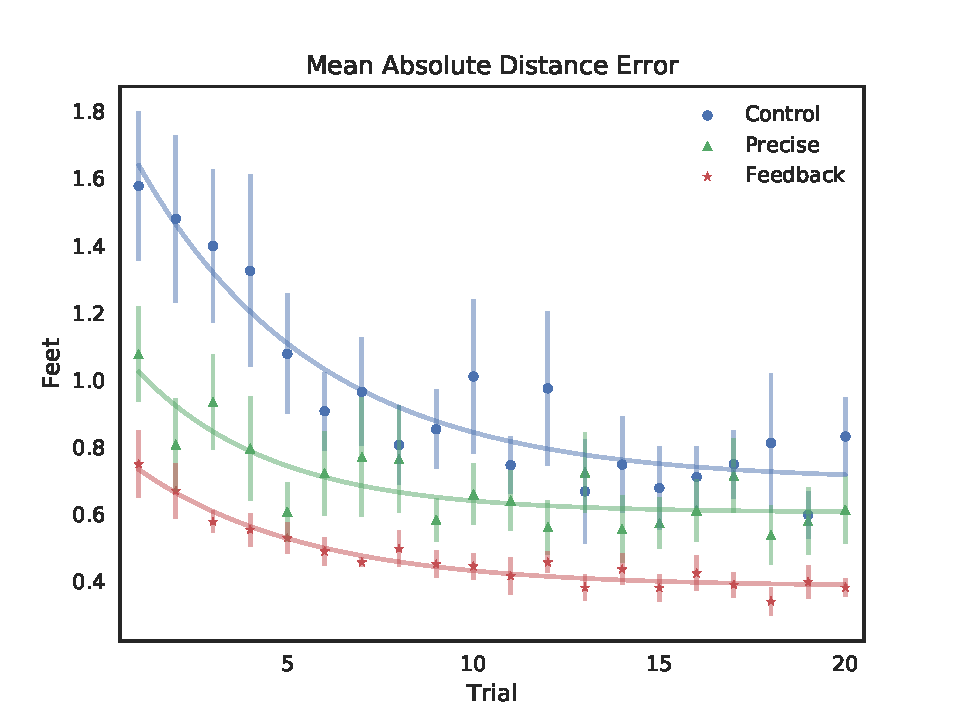
\includegraphics[width=\textwidth]{../img/Group_absDistErr_clean_fit_30.pdf}
  \end{center}
\end{frame}

\begin{frame}[fragile]{SAFER Workload}
  \begin{center}
    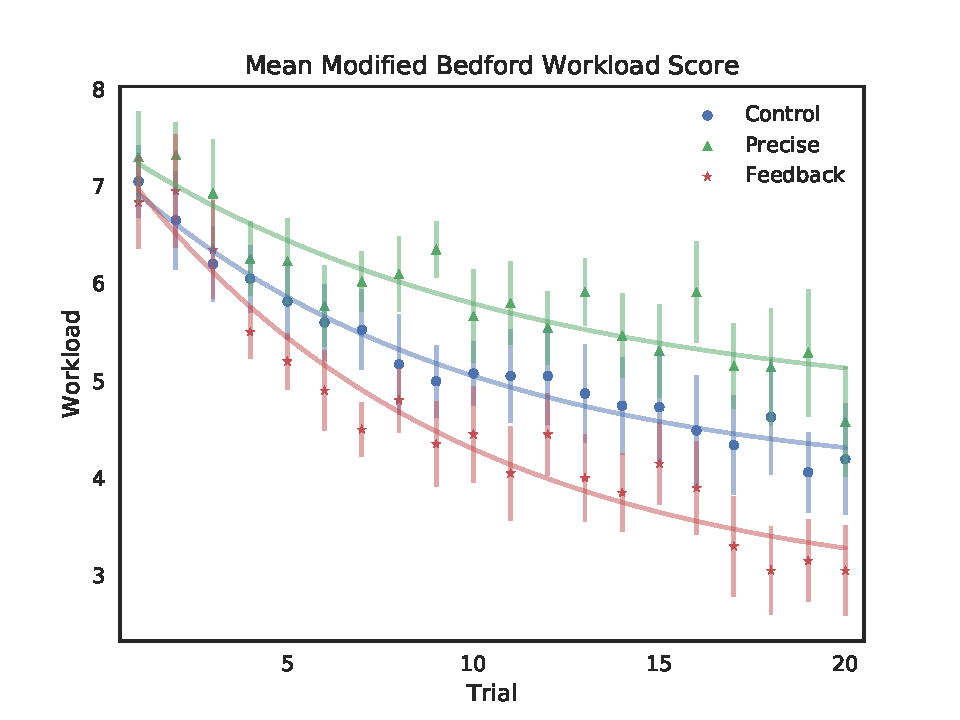
\includegraphics[width=\textwidth]{../img/Group_Workload_fit_30.pdf}
  \end{center}
\end{frame}

\begin{frame}[fragile]{Sigrist et al., 2013~\cite{Sigrist2013}}
  \begin{center}
    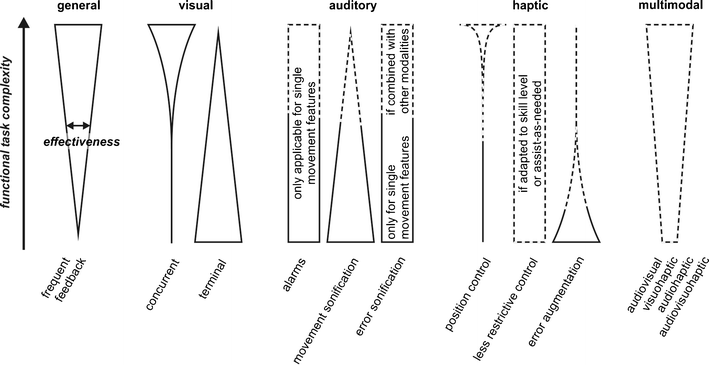
\includegraphics[width=\textwidth]{../img/sigrist.png}
  \end{center}
\end{frame}

\section{Proposed Research}

\subsection{Experiment One}

\begin{frame}[fragile]{Motivation}
  \begin{itemize}
    \setlength\itemsep{1em}
    \item Link Foundation Modeling, Simulation, and Training Fellowship
    \item Measure the effects of augmented reality on performance and workload in robotics training
    \item Hypothesize that AR would improve performance
  \end{itemize}
\end{frame}

\begin{frame}[fragile]{Three-axis tracking task designs}
  \begin{figure}
    \begin{center}
      \begin{subfigure}{0.45\linewidth}
        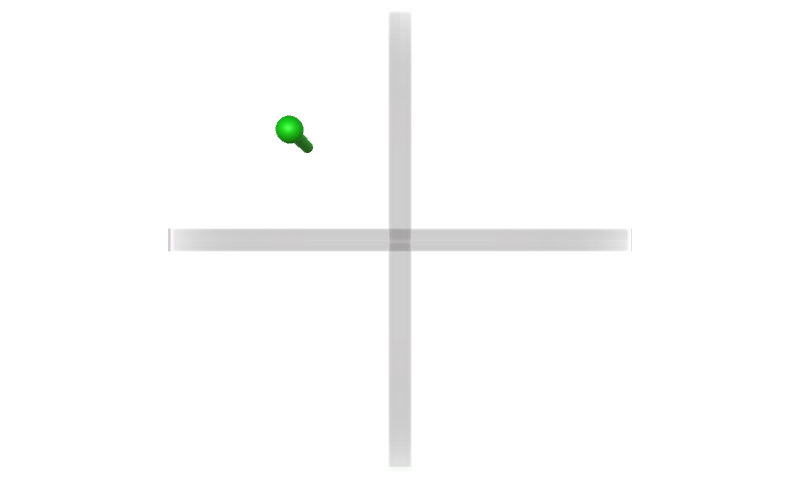
\includegraphics[width=\linewidth]{../img/Baseline.png}
        \caption{Baseline}
      \end{subfigure}\hfill
      \begin{subfigure}{0.45\linewidth}
        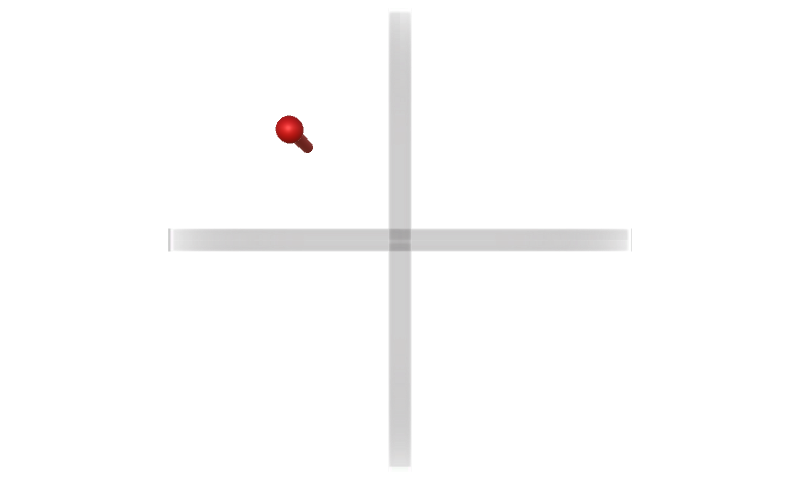
\includegraphics[width=\linewidth]{../img/Color.png}
        \caption{Feedback}
      \end{subfigure}\hfill
      \begin{subfigure}{0.45\linewidth}
        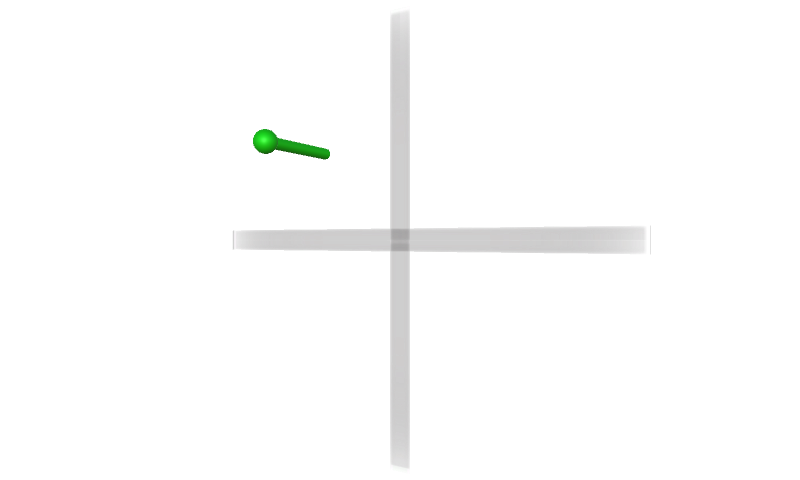
\includegraphics[width=\linewidth]{../img/Angled.png}
        \caption{Rotated}
      \end{subfigure}
      % \caption{The fixed-based simulator used by both groups.}%
      % \label{fig:simulator}%
    \end{center}
  \end{figure}
\end{frame}

\begin{frame}[fragile]{Three-axis tracking groups}
  \begin{figure}
    \begin{center}
      \begin{subfigure}{0.49\textwidth}
        \includegraphics[width=\linewidth]{../img/DSC_0801.JPG}
        \caption{2D Group}
      \end{subfigure}\hfill
      \begin{subfigure}{0.49\textwidth}
        \includegraphics[width=\linewidth]{../img/DSC_0803.JPG}
        \caption{3D Group}
      \end{subfigure}
      % \caption{The fixed-based simulator used by both groups.}%
      % \label{fig:simulator}%
    \end{center}
  \end{figure}
\end{frame}

\begin{frame}[fragile]{Three-axis tracking}
  \begin{center}
    \newcommand\vidname{videos/tracking.mp4}   %path to video (must be subdir)
    \newcommand\thumbname{../img/DSC_0811.JPG} %path to thumbnail
    \newcommand\moviewidth{1.0\textwidth}
    \includemedia[
      width=\moviewidth,
      % totalheight=0.225\linewidth,
      activate=pageopen,
      passcontext,  %show VPlayer's right-click menu
      addresource=\vidname,
      flashvars={
          source=\vidname %important: same path as in `addresource'
          % &autoPlay=true
          % &scaleMode=letterbox
          &loop=true
        }
    ]{\includegraphics[width=\moviewidth]{\thumbname}}{VPlayer.swf}
  \end{center}
\end{frame}

\begin{frame}[fragile]{Performance Analysis}
\begin{figure}
  \begin{center}
    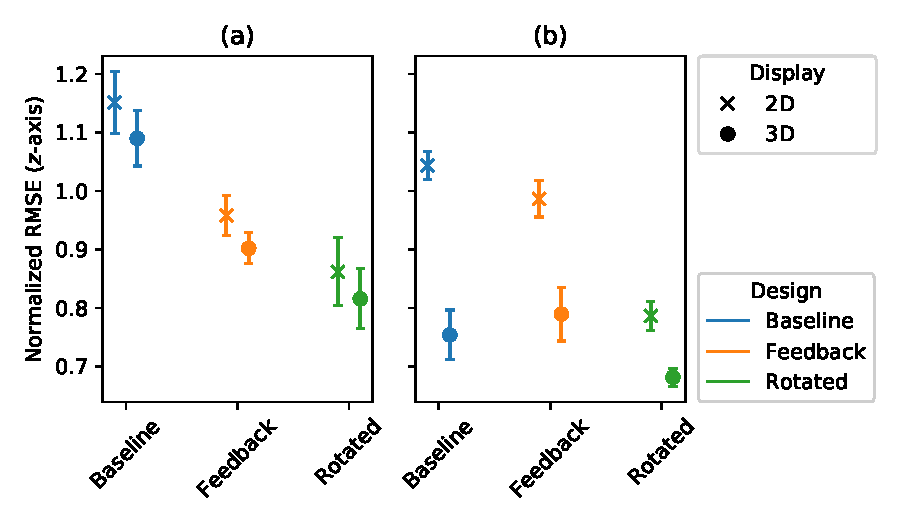
\includegraphics[width=\linewidth]{../img/2way.pdf}
  \end{center}
\end{figure}
\end{frame}

\begin{frame}[fragile]{Workload Analysis}
\begin{figure}
  \begin{center}
    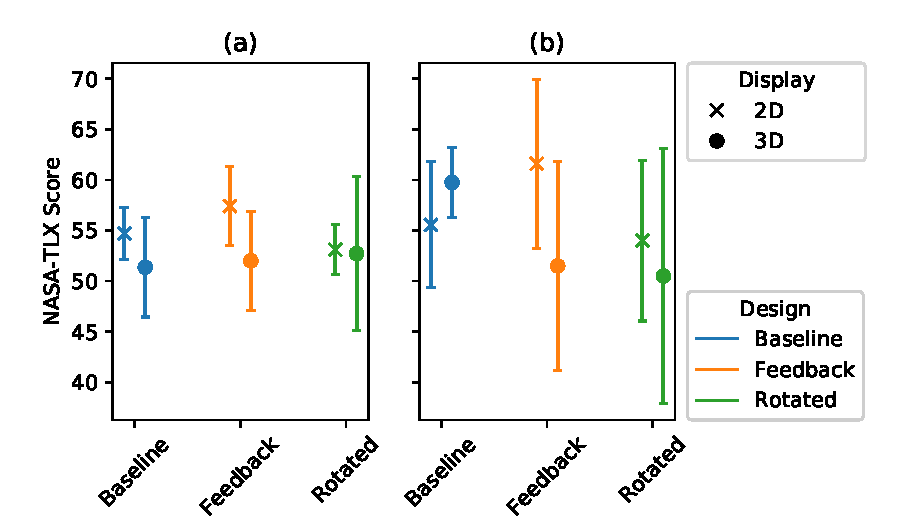
\includegraphics[width=\linewidth]{../img/2way-work.pdf}
  \end{center}
\end{figure}
\end{frame}

\begin{frame}[fragile]{Result Summary}
  \begin{itemize}
    \setlength\itemsep{1em}
    \item Feedback improves performance
    \item Better performance in 3D, but only when starting with feedback
    \item No changes in workload
  \end{itemize}
\end{frame}

\subsection{Experiment Two}

\begin{frame}[fragile]{Canadarm2}
  \begin{columns}[T]
    \begin{column}{.4\textwidth}
      \begin{itemize}
        \setlength\itemsep{1em}
        \item <1->Launched 2001, 7~DoF, 60~feet long, 4000~lb
        \item <2->Astronaut EVA Assist
        \item <3->Grappling visiting vehicles
      \end{itemize}
    \end{column}
    \begin{column}{.6\textwidth}
      \begin{tikzpicture}
        \node<1> (img1) {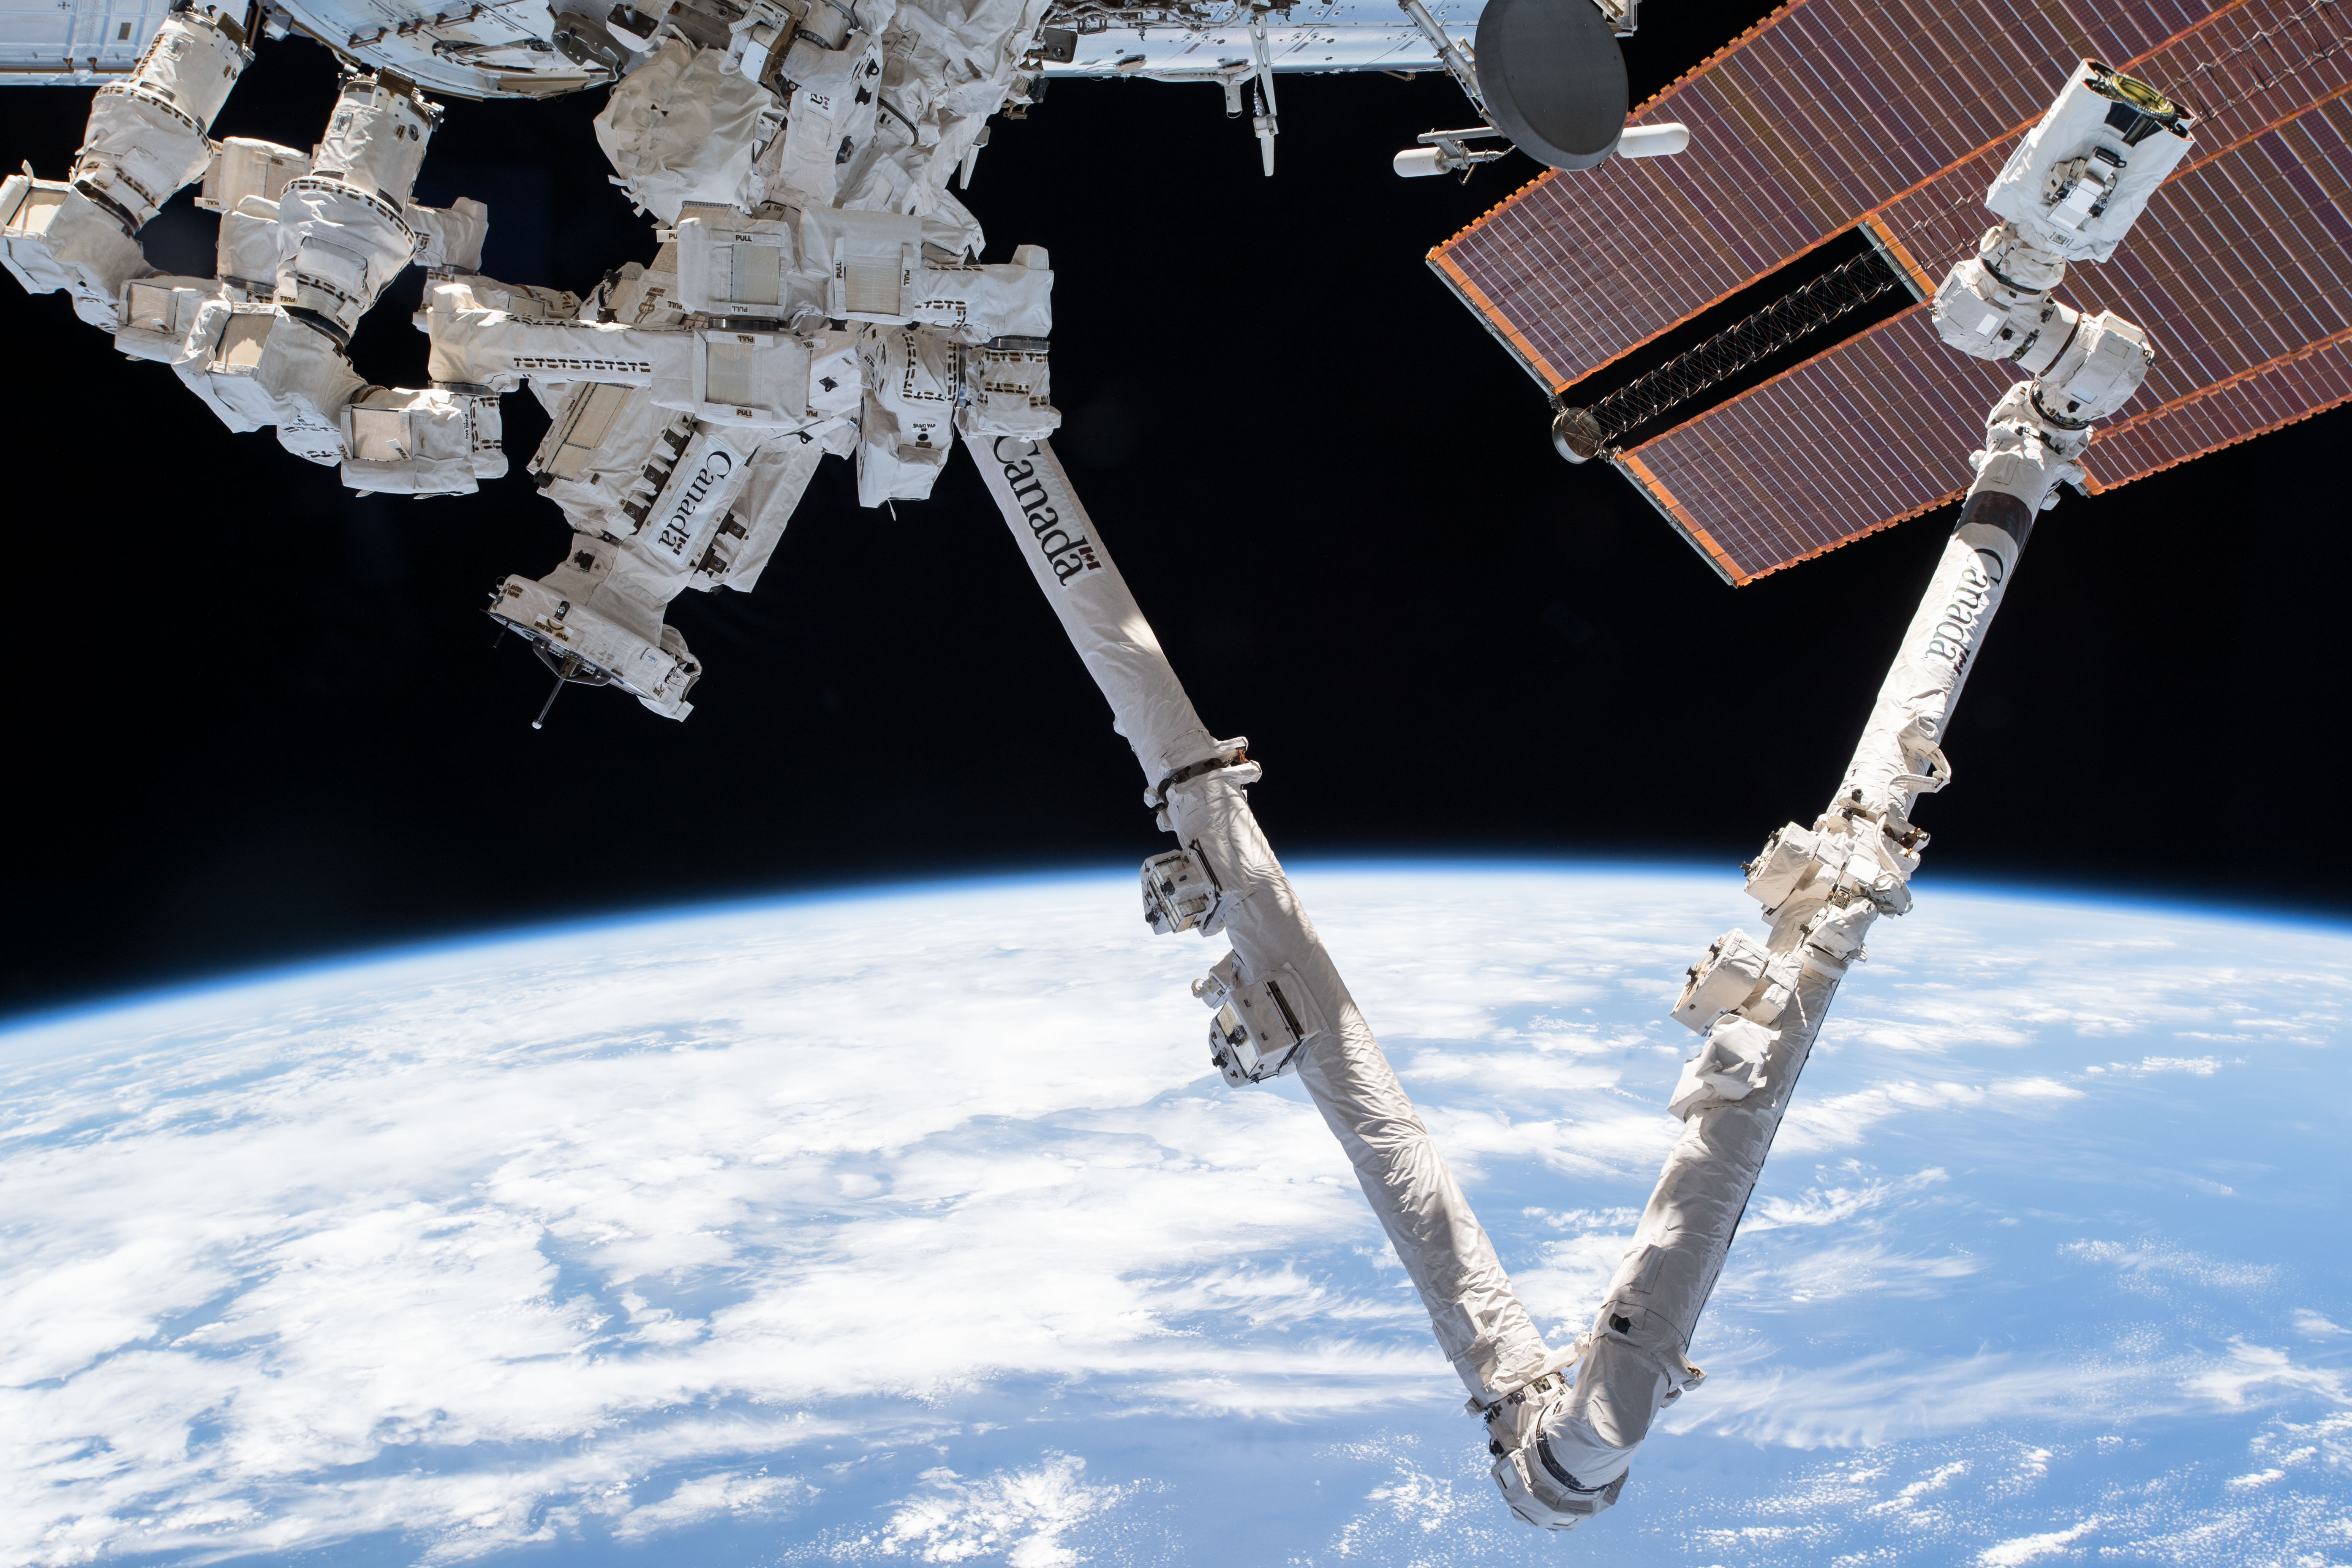
\includegraphics[height=0.7\linewidth, width=\textwidth]{../img/canadarm2.jpg}};
        \node<2> (img2) {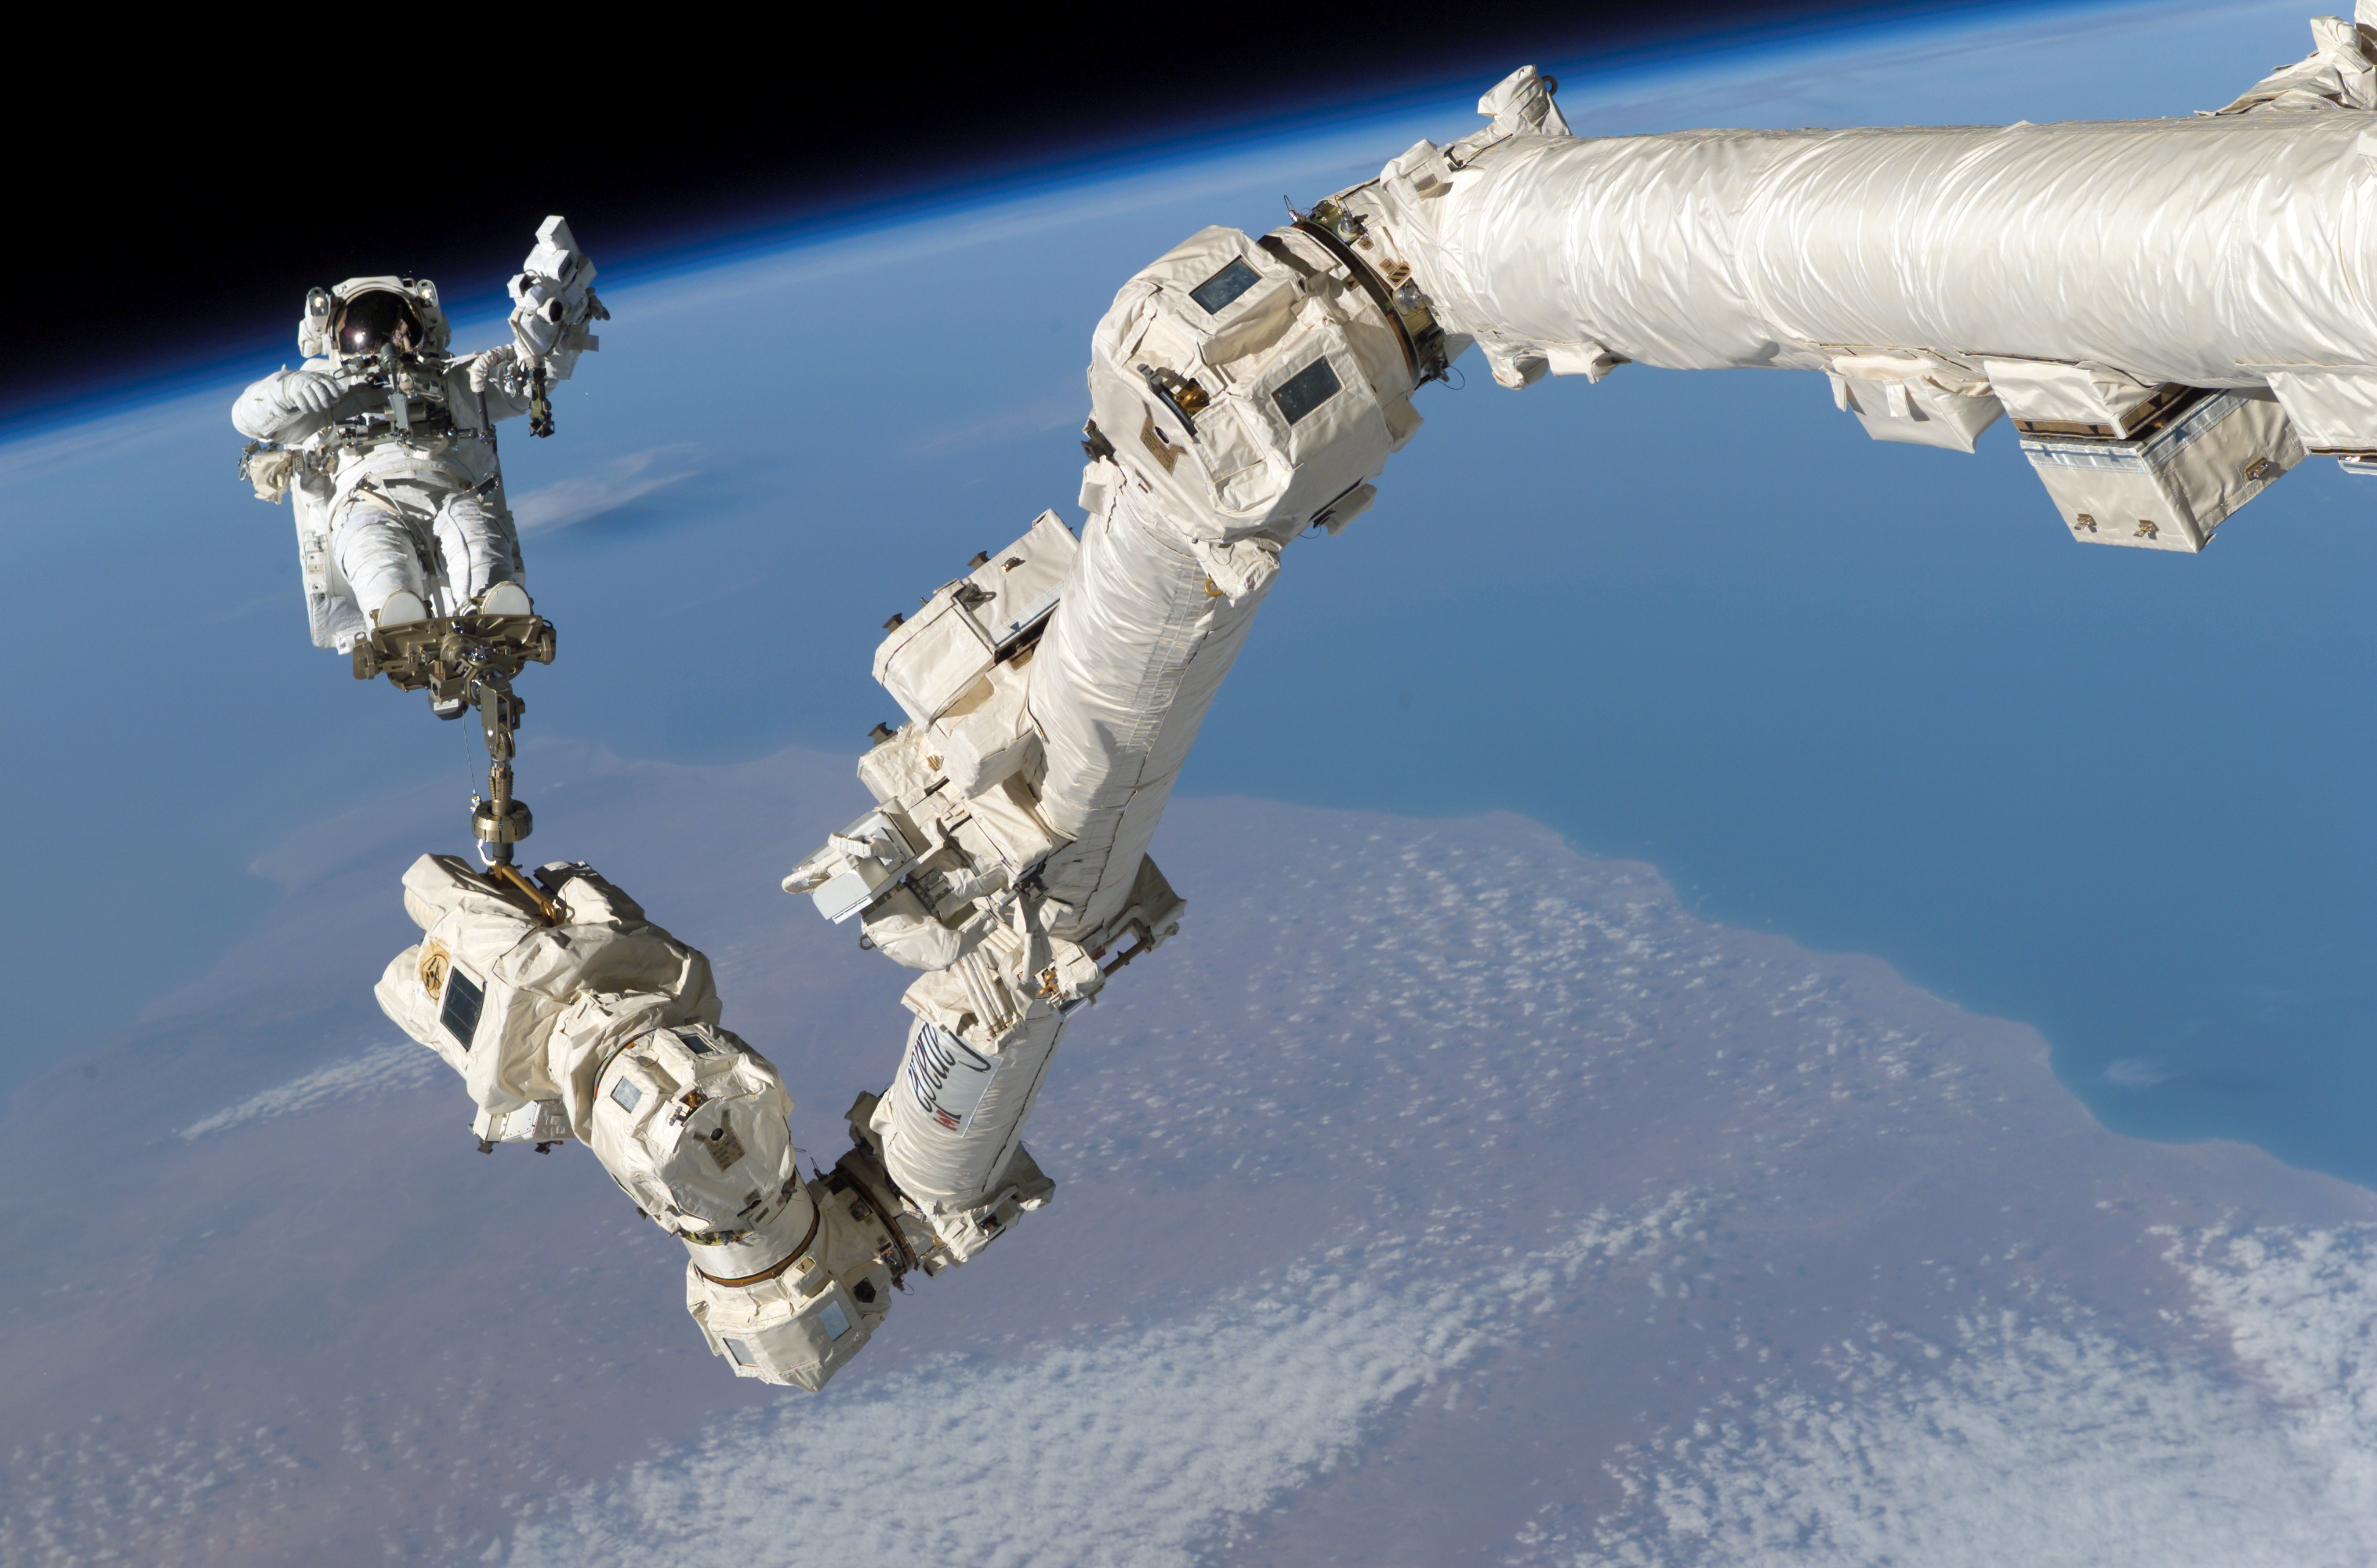
\includegraphics[height=0.7\linewidth, width=\textwidth]{../img/STS-114_Steve_Robinson_on_Canadarm2.jpg}};
        \node<3> (img3) {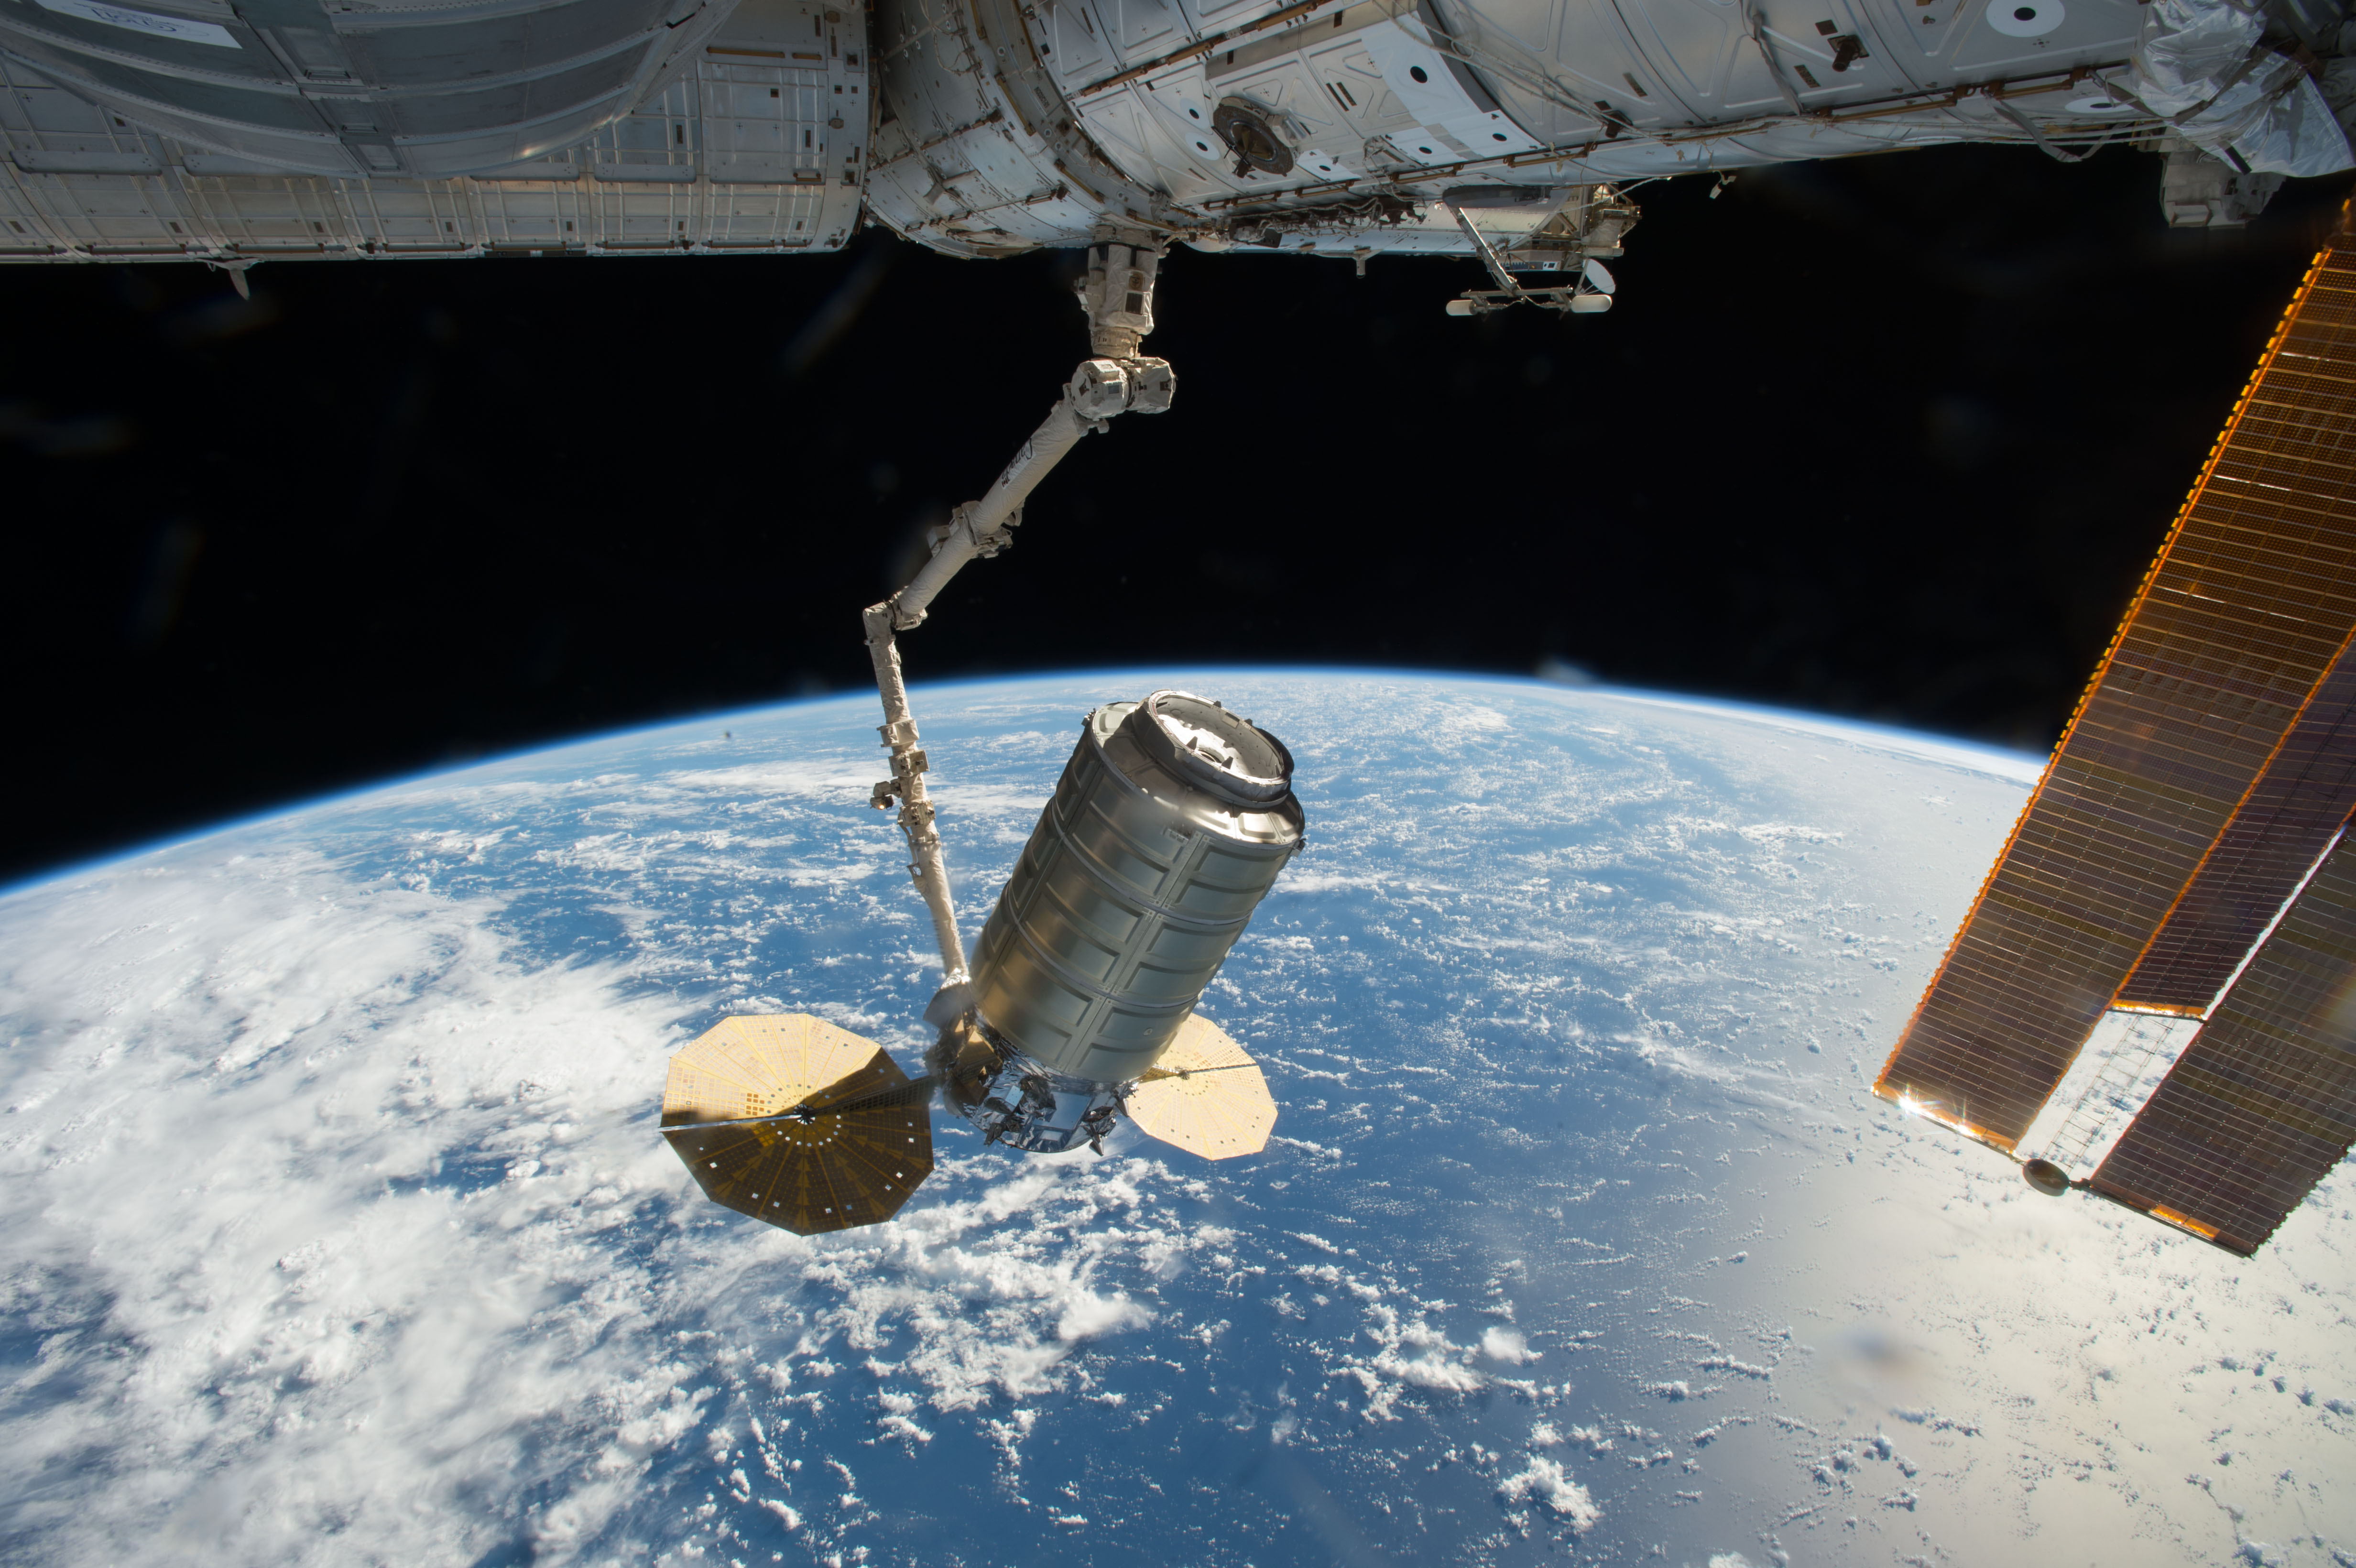
\includegraphics[height=0.7\linewidth, width=\textwidth]{../img/Cygnus_7_captured_by_Canadarm2.jpg}};
      \end{tikzpicture}
    \end{column}
  \end{columns}
\end{frame}

\begin{frame}[fragile]{RWS on ISS}
  \begin{figure}
    \begin{center}
      \begin{subfigure}{0.49\textwidth}
        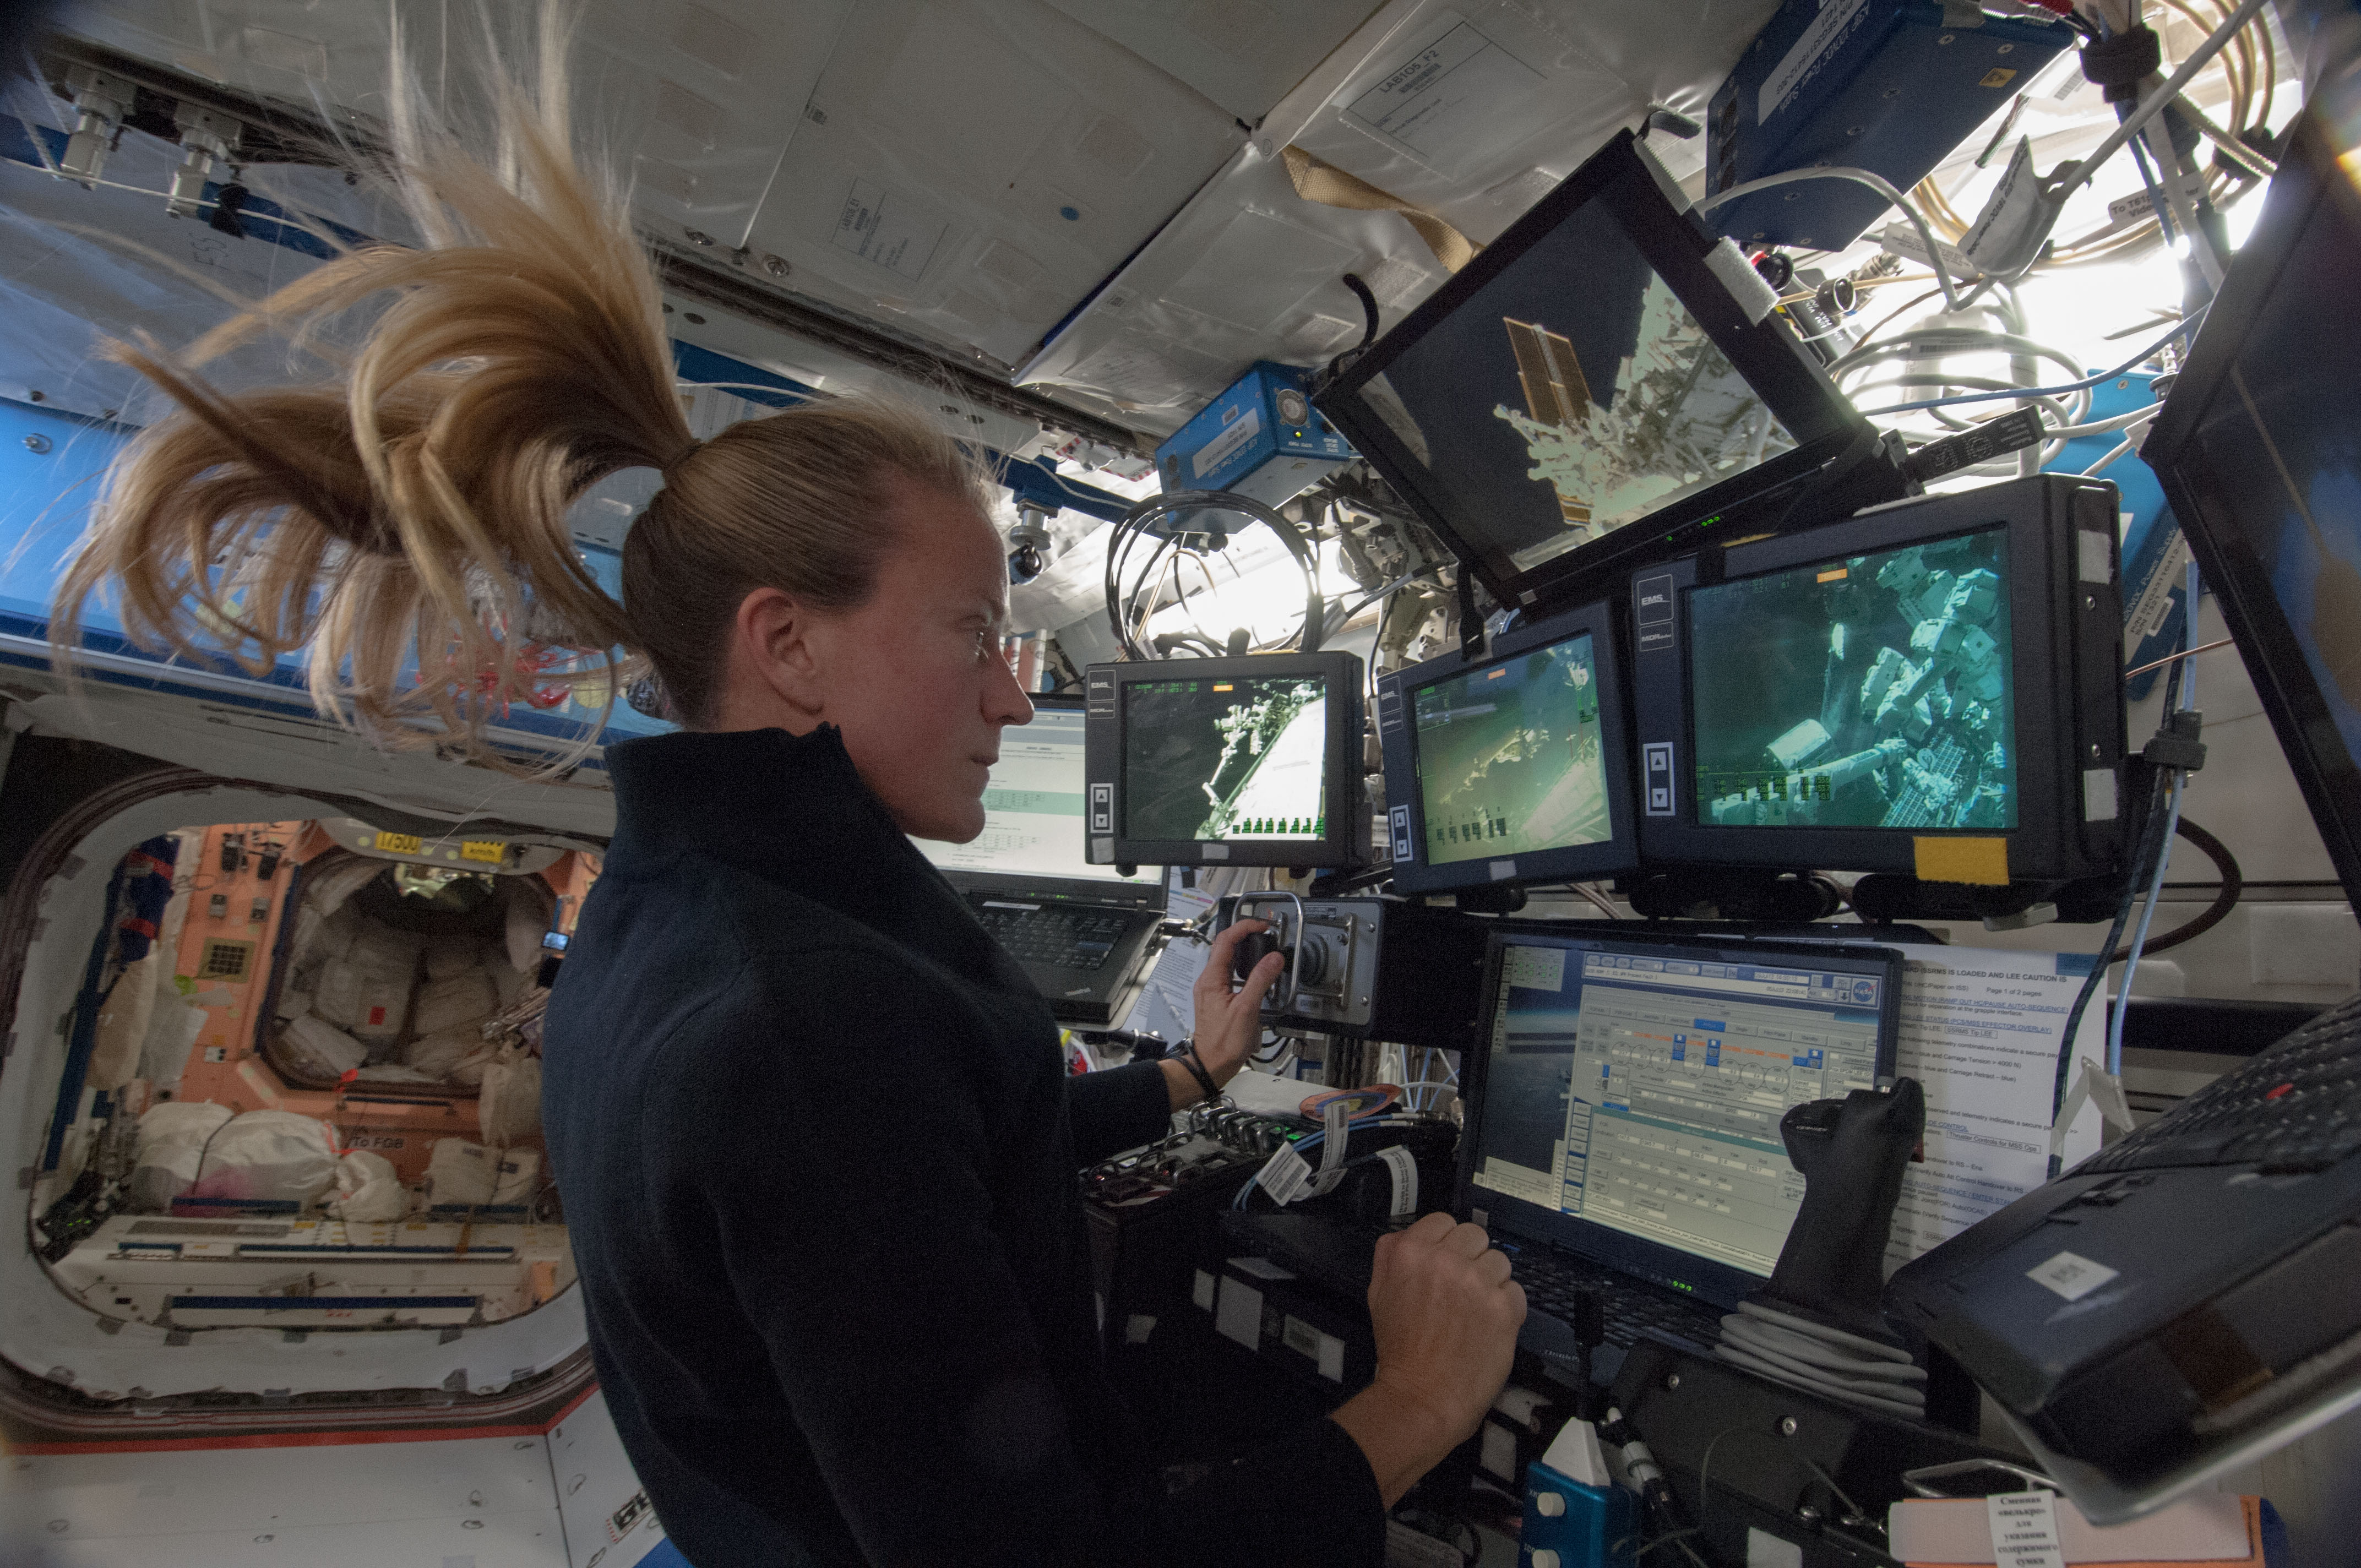
\includegraphics[width=\linewidth]{../img/iss036e017589.JPG}
        \caption{Node Module}
      \end{subfigure}\hfill
      \begin{subfigure}{0.49\textwidth}
        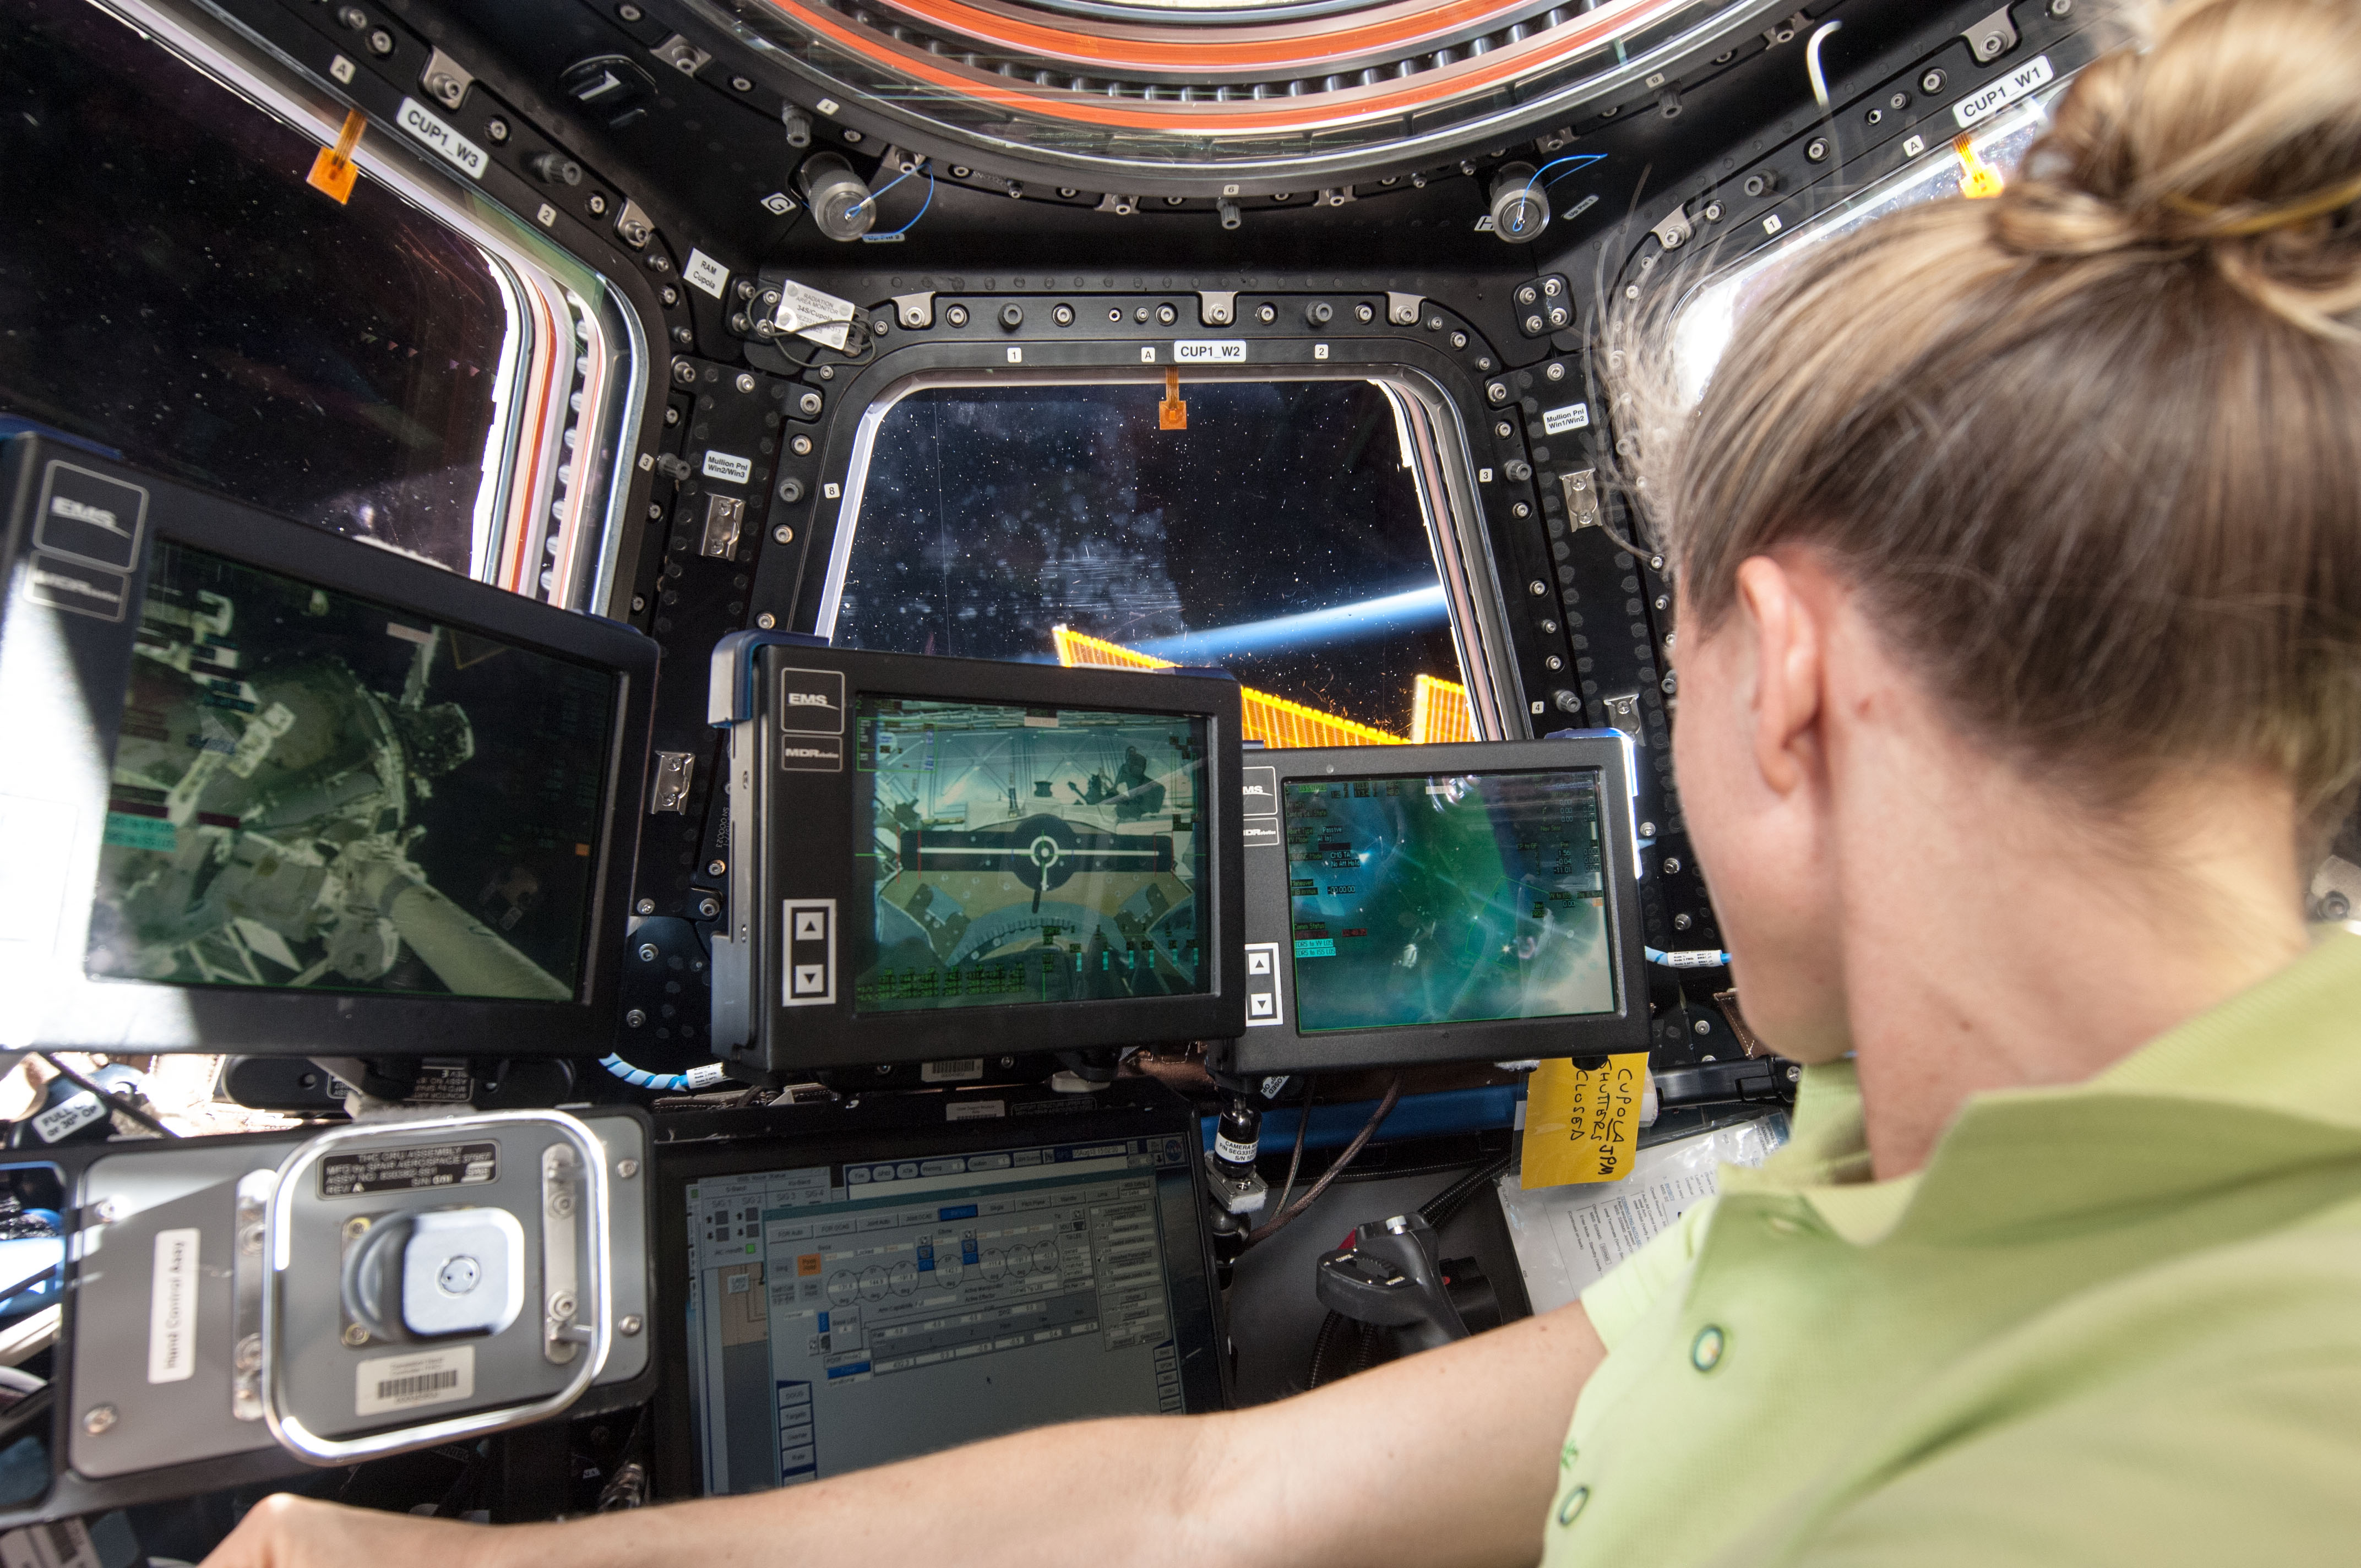
\includegraphics[width=\linewidth]{../img/iss036e029229.JPG}
        \caption{Cupola}
      \end{subfigure}
      % \caption{The fixed-based simulator used by both groups.}%
      % \label{fig:simulator}%
    \end{center}
  \end{figure}
\end{frame}

\begin{frame}[fragile]{Cupola Provides an Extra View}
  \begin{center}
    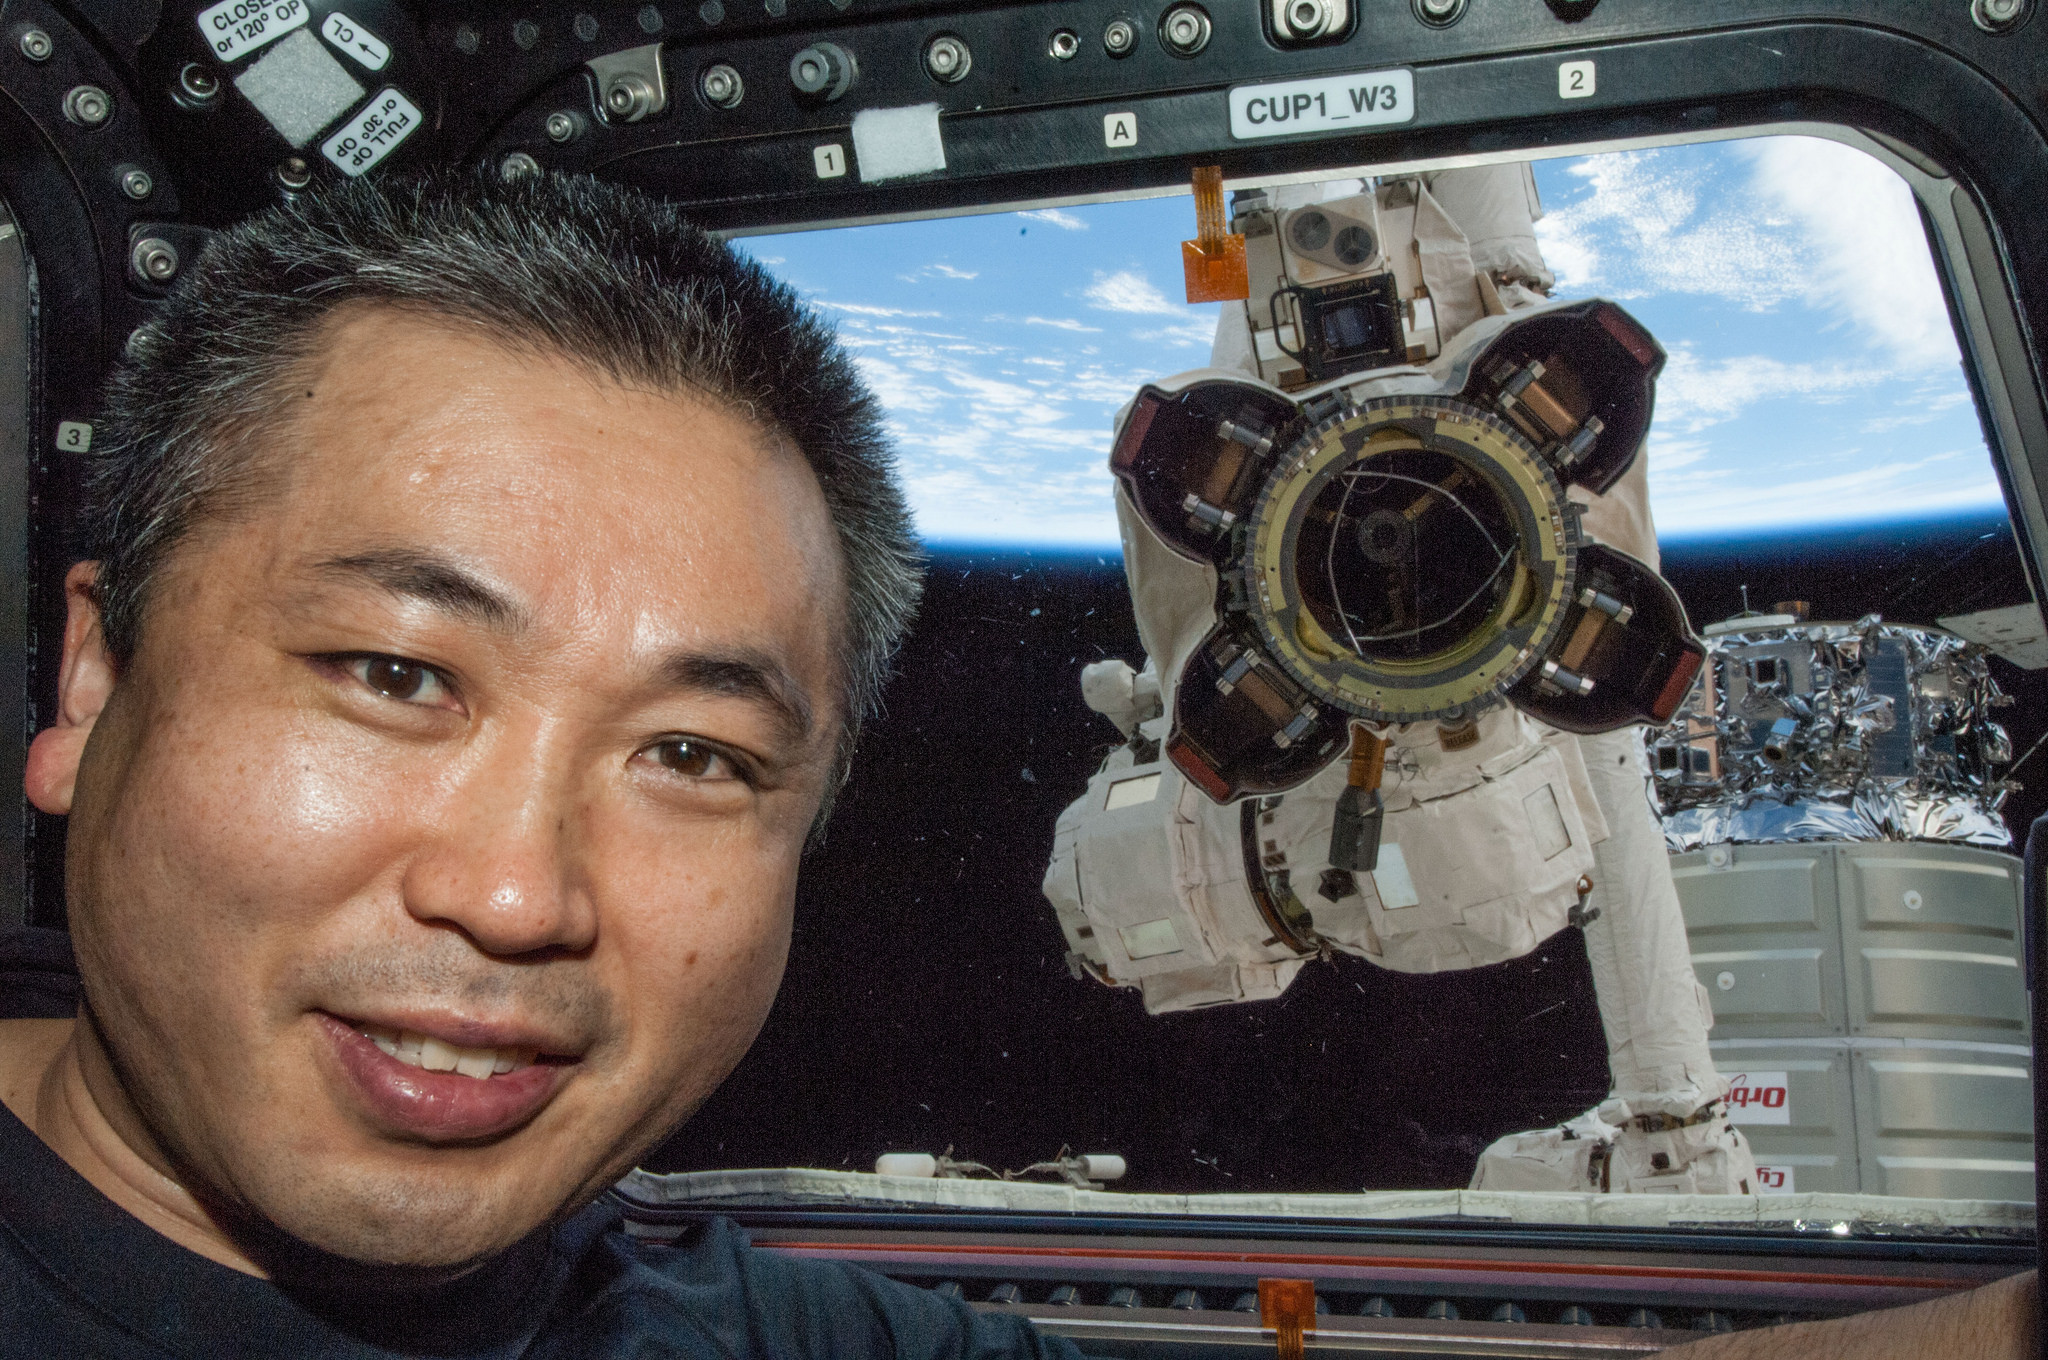
\includegraphics[width=\textwidth]{../img/12085915275_c7f77c537e_k.jpg}
  \end{center}
\end{frame}

\begin{frame}[fragile]{Track and Capture Scenario}
  \begin{itemize}
    \setlength\itemsep{1em}
    \item Vehicle arrives at capture point
    \item ISS and vehicle in two separate, nearby orbits
    \item Operators must capture a vehicle drifting in six dimensions
  \end{itemize}
\end{frame}

\begin{frame}[fragile]{The Task}
  \begin{columns}[T]
    \begin{column}{\textwidth}
      \begin{tikzpicture}
        \node<1> (img1) {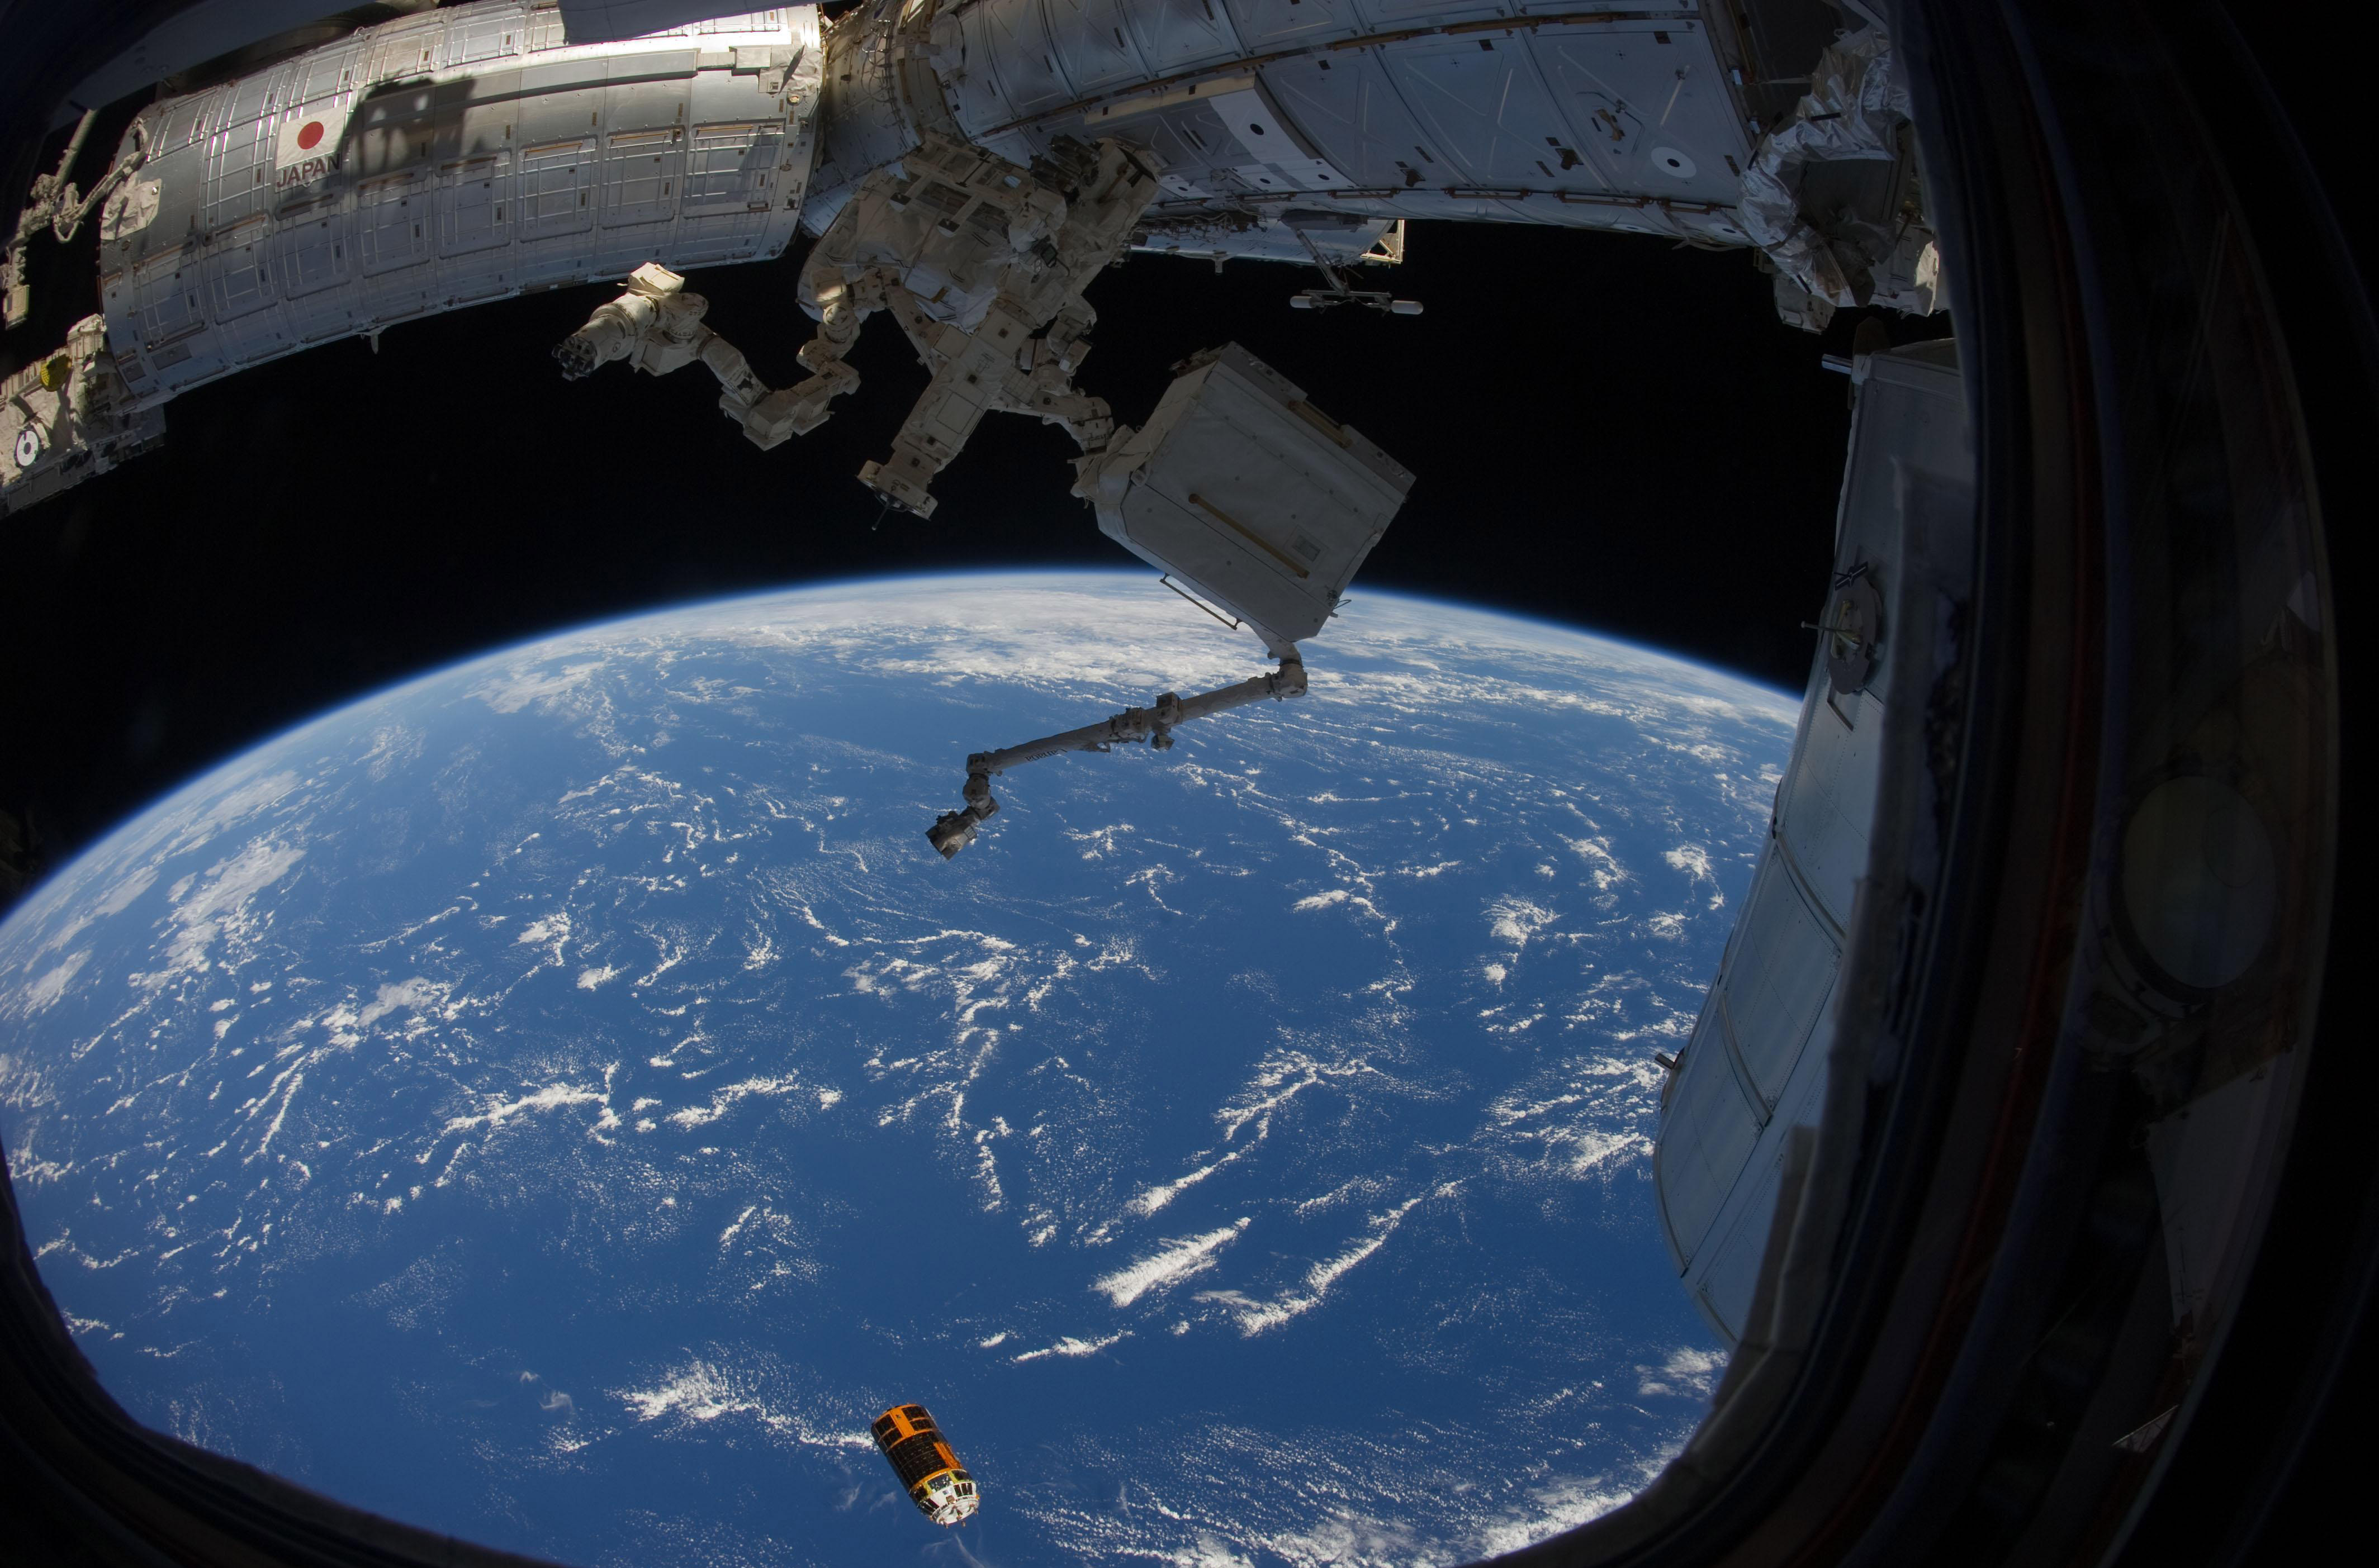
\includegraphics[width=\textwidth]{../img/grab1.jpg}};
        \node<2> (img2) {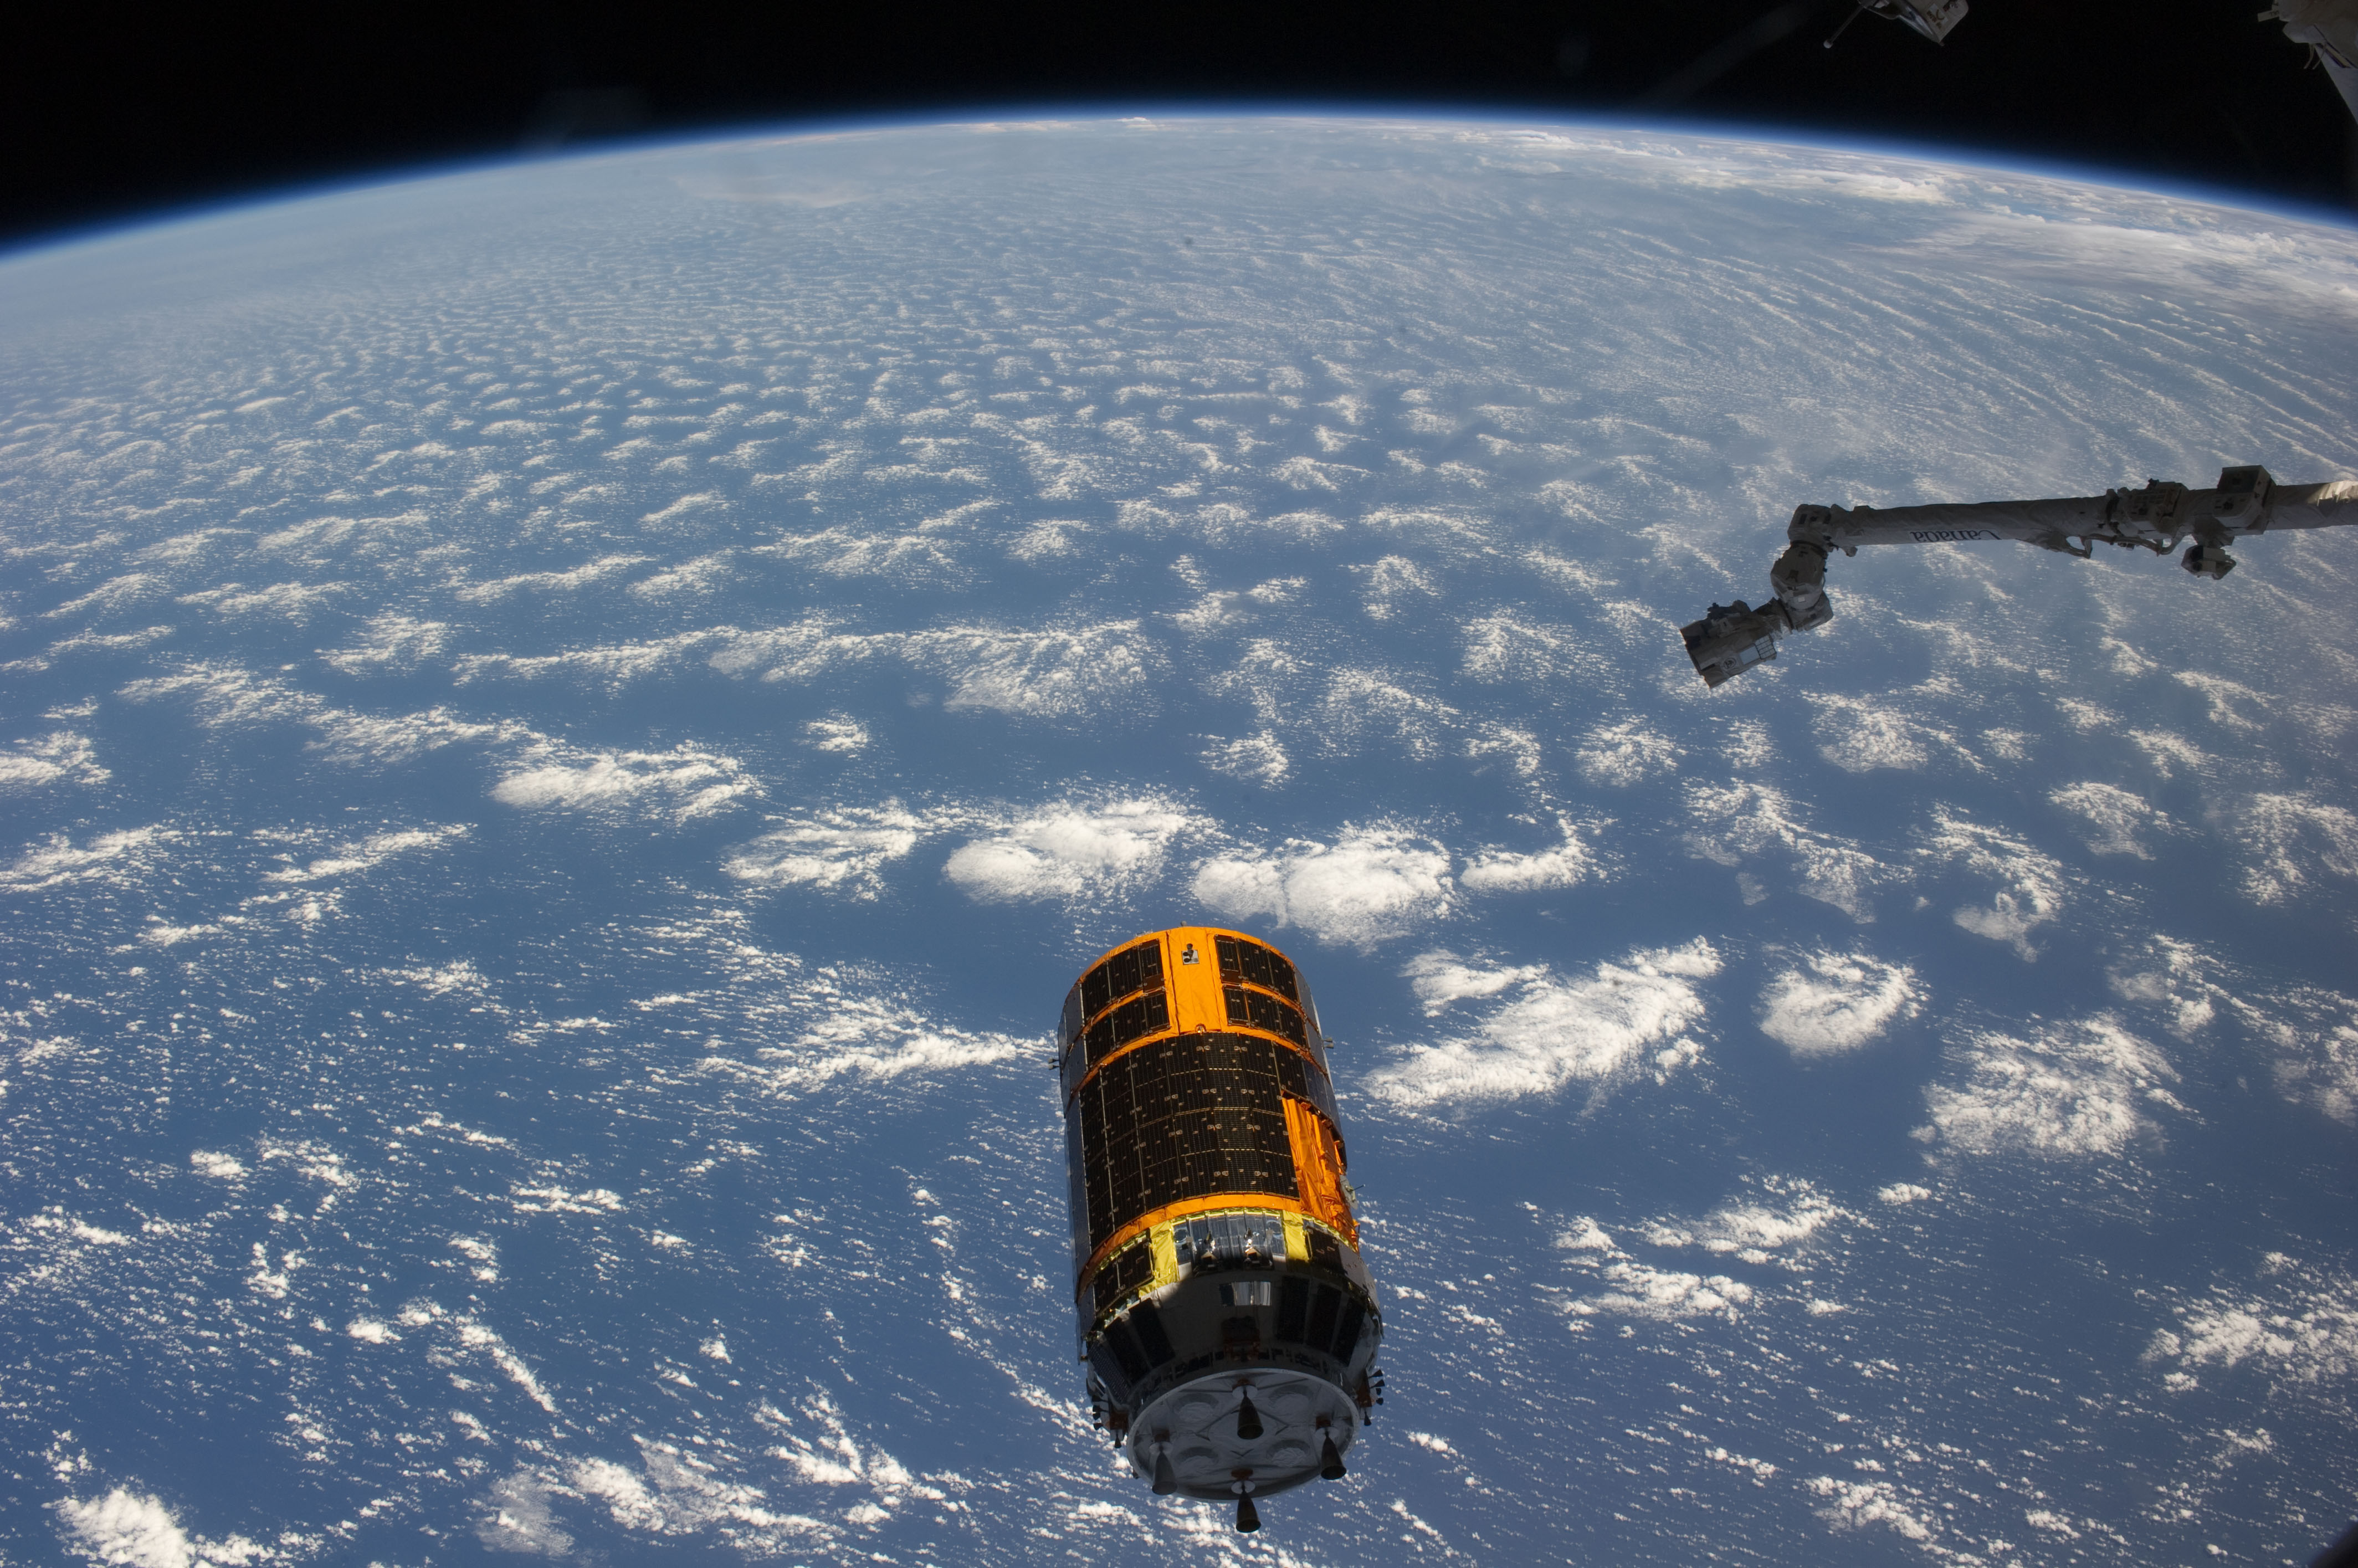
\includegraphics[width=\textwidth]{../img/grab2.jpg}};
        \node<3> (img3) {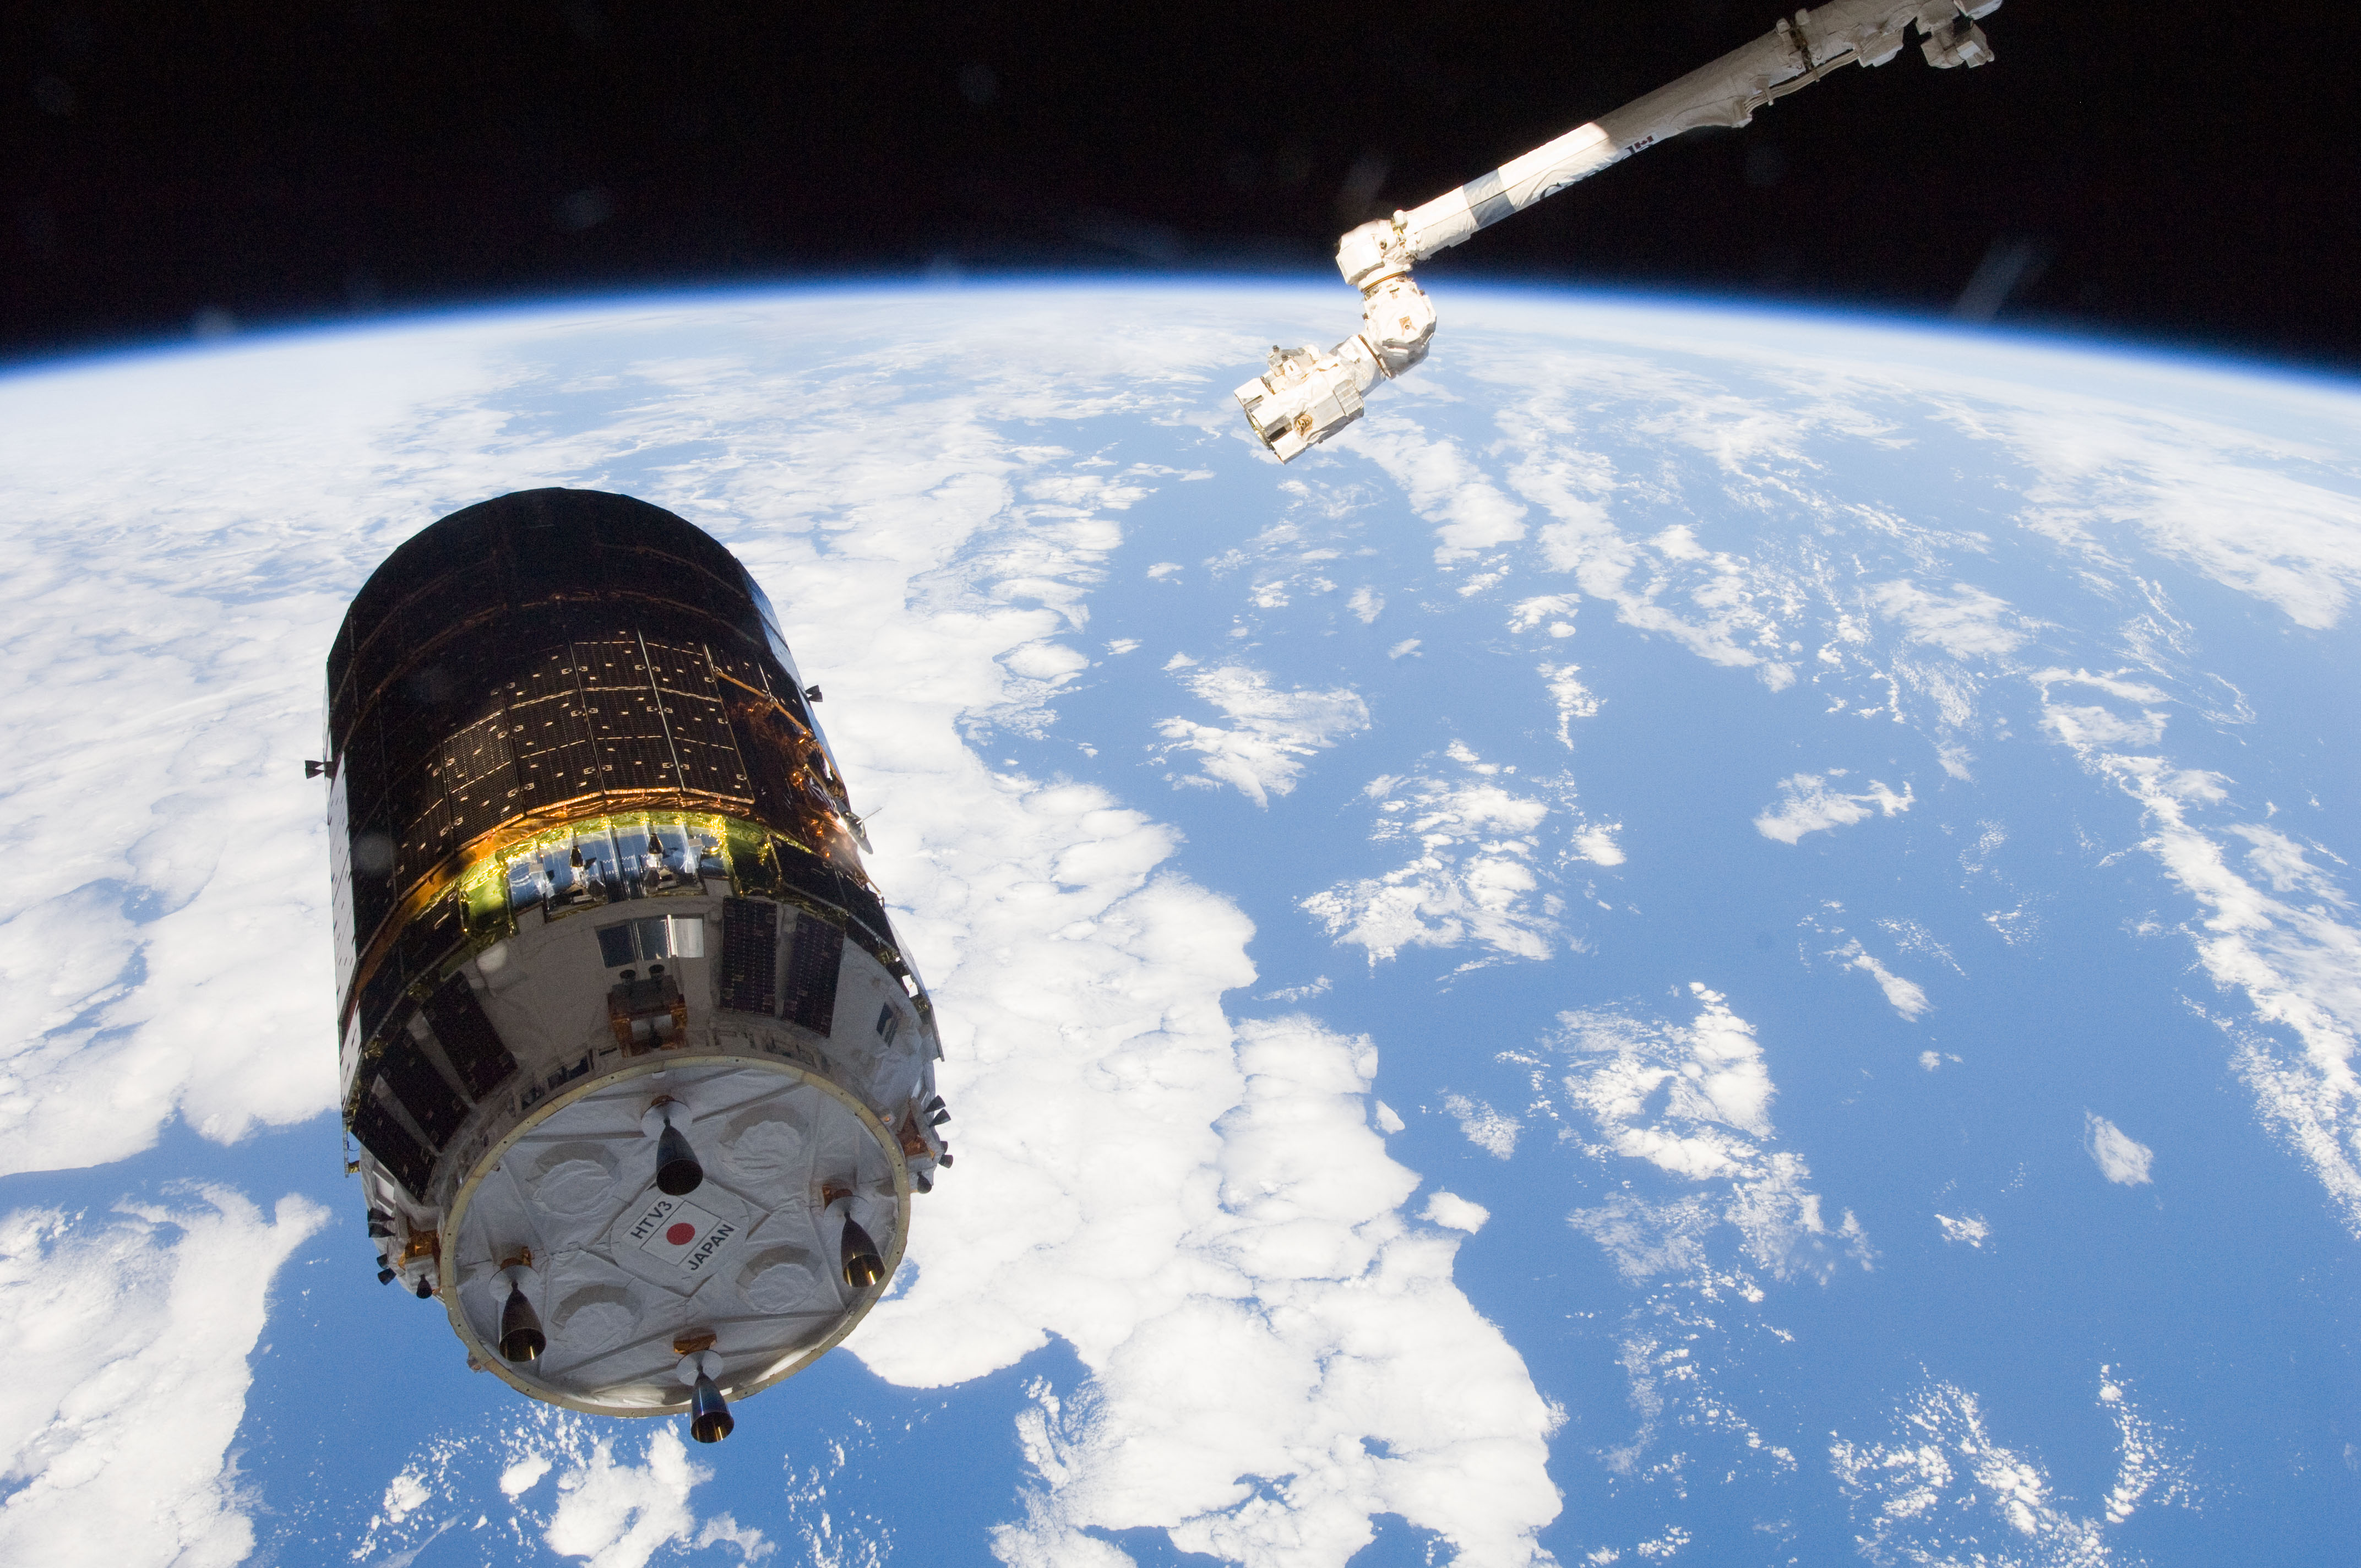
\includegraphics[width=\textwidth]{../img/grab3.jpg}};
        \node<4> (img4) {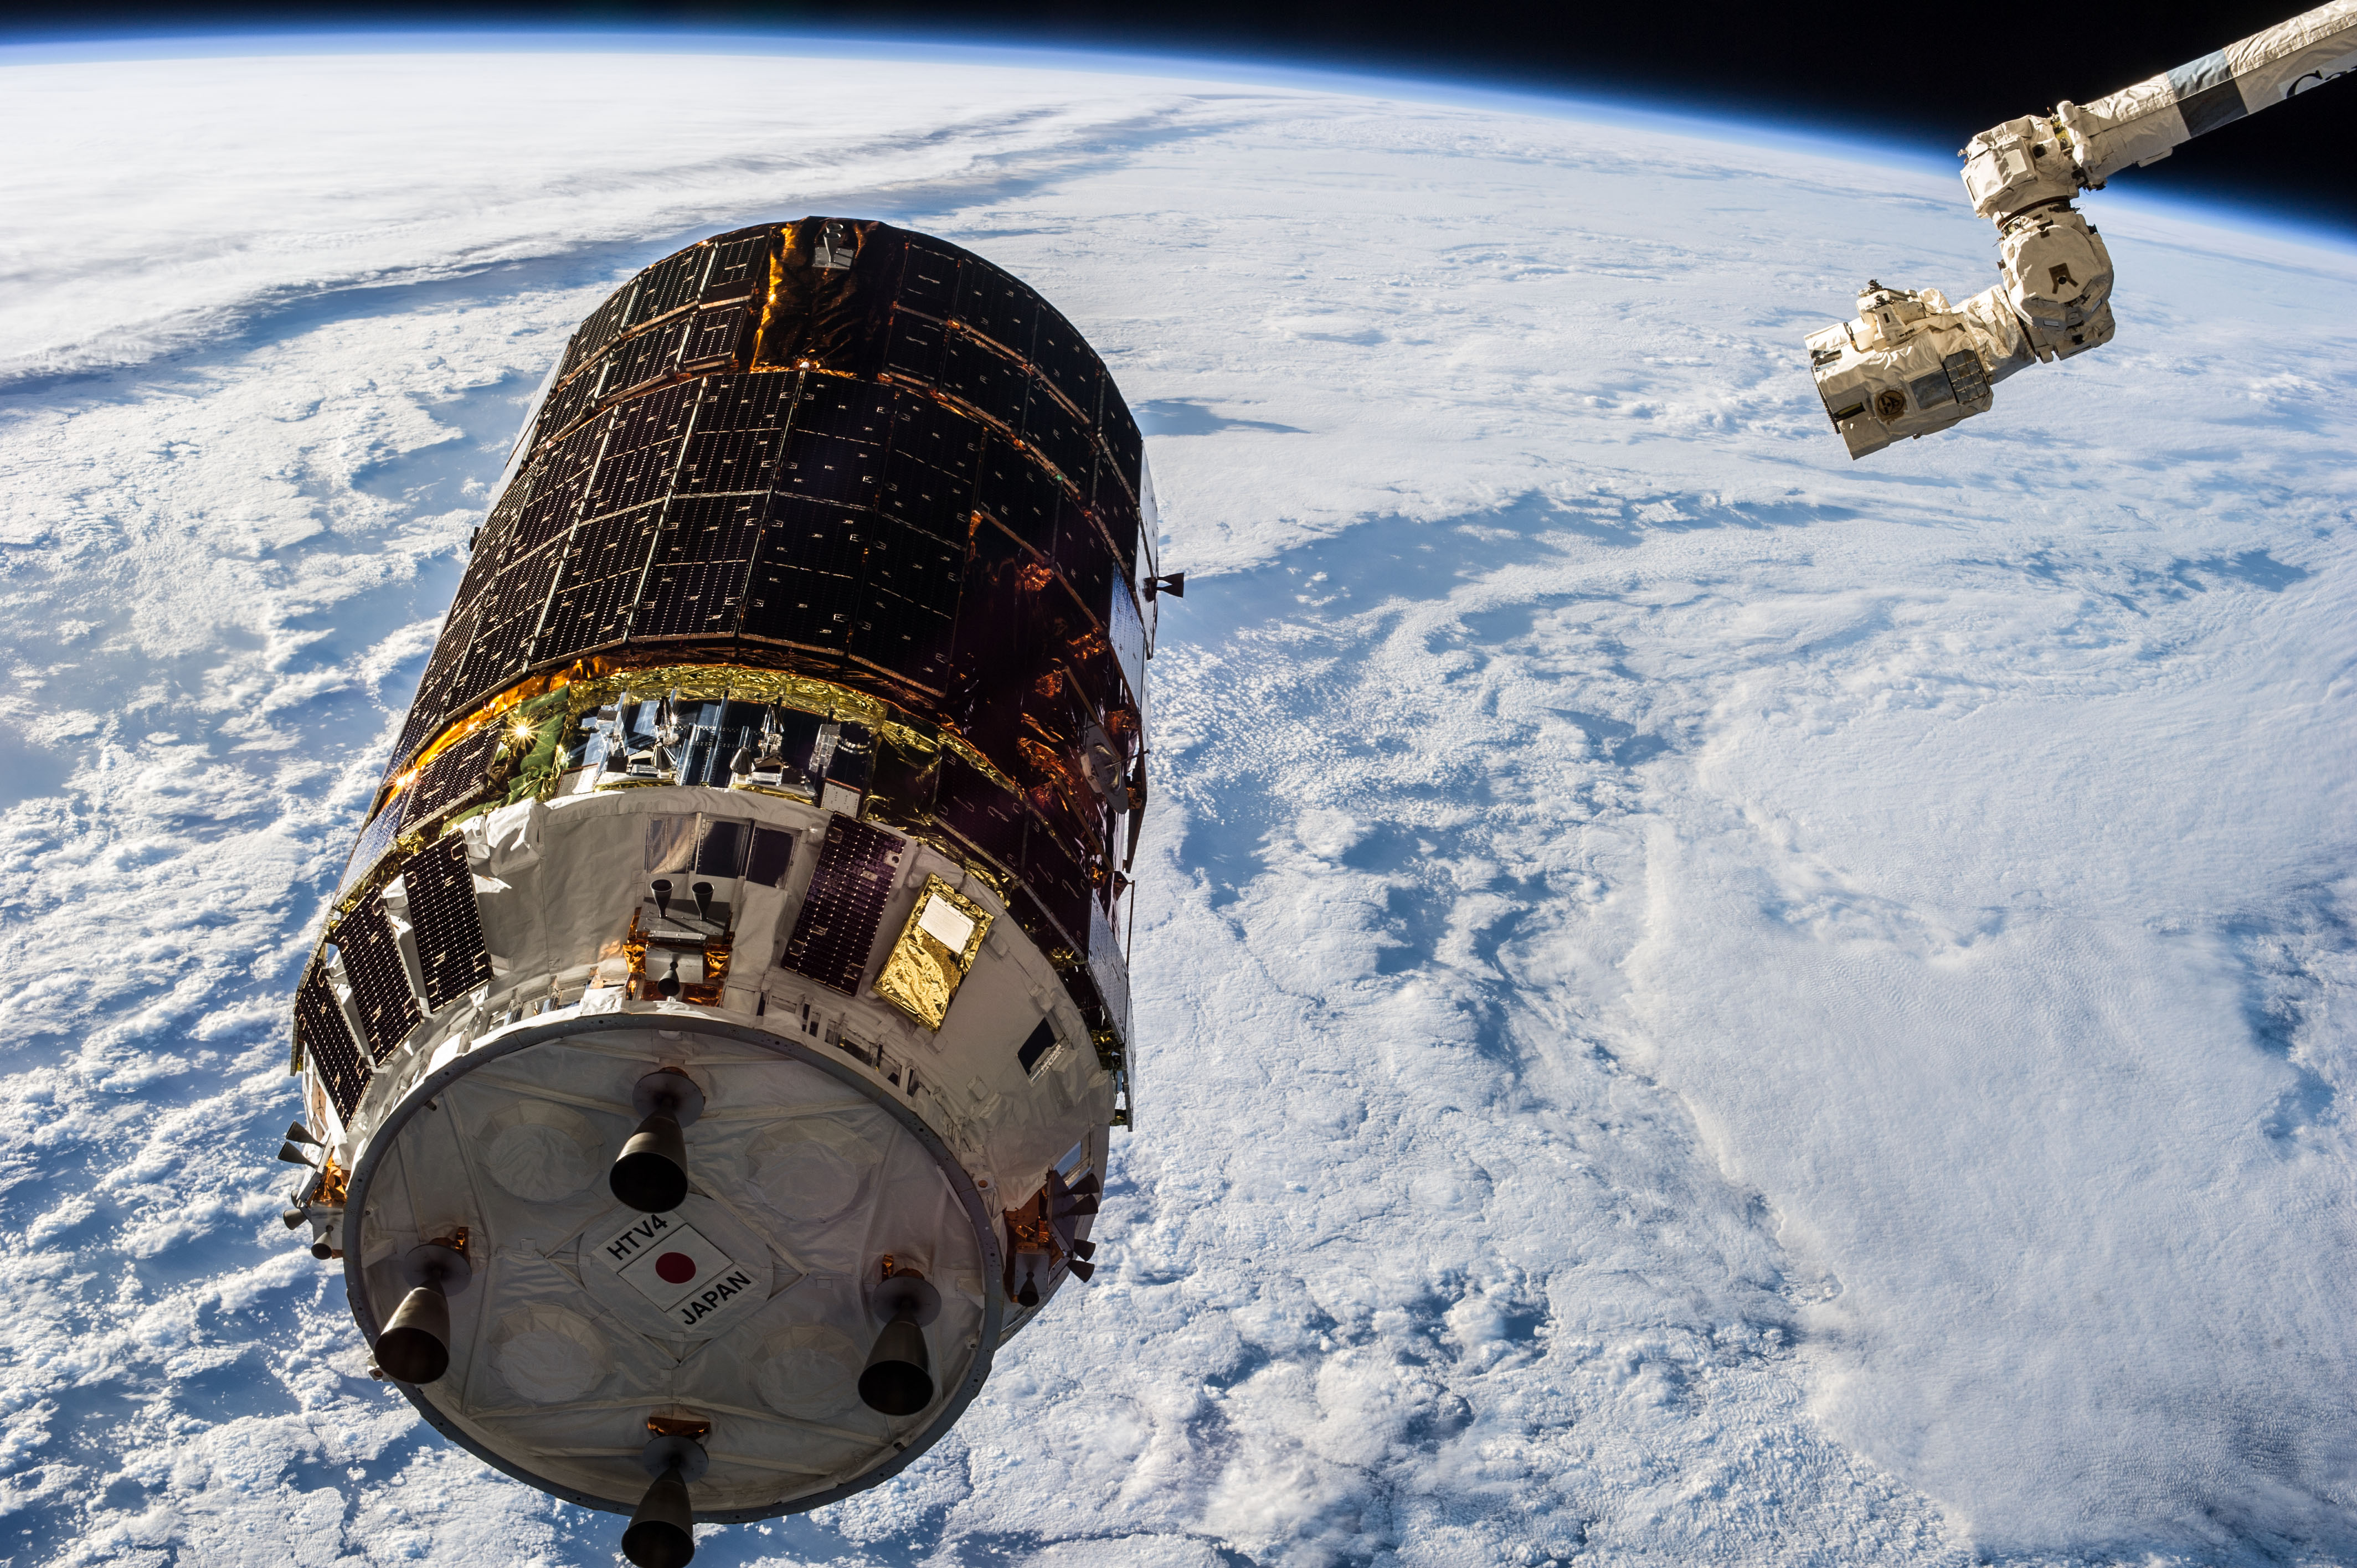
\includegraphics[width=\textwidth]{../img/grab4.jpg}};
        \node<5> (img5) {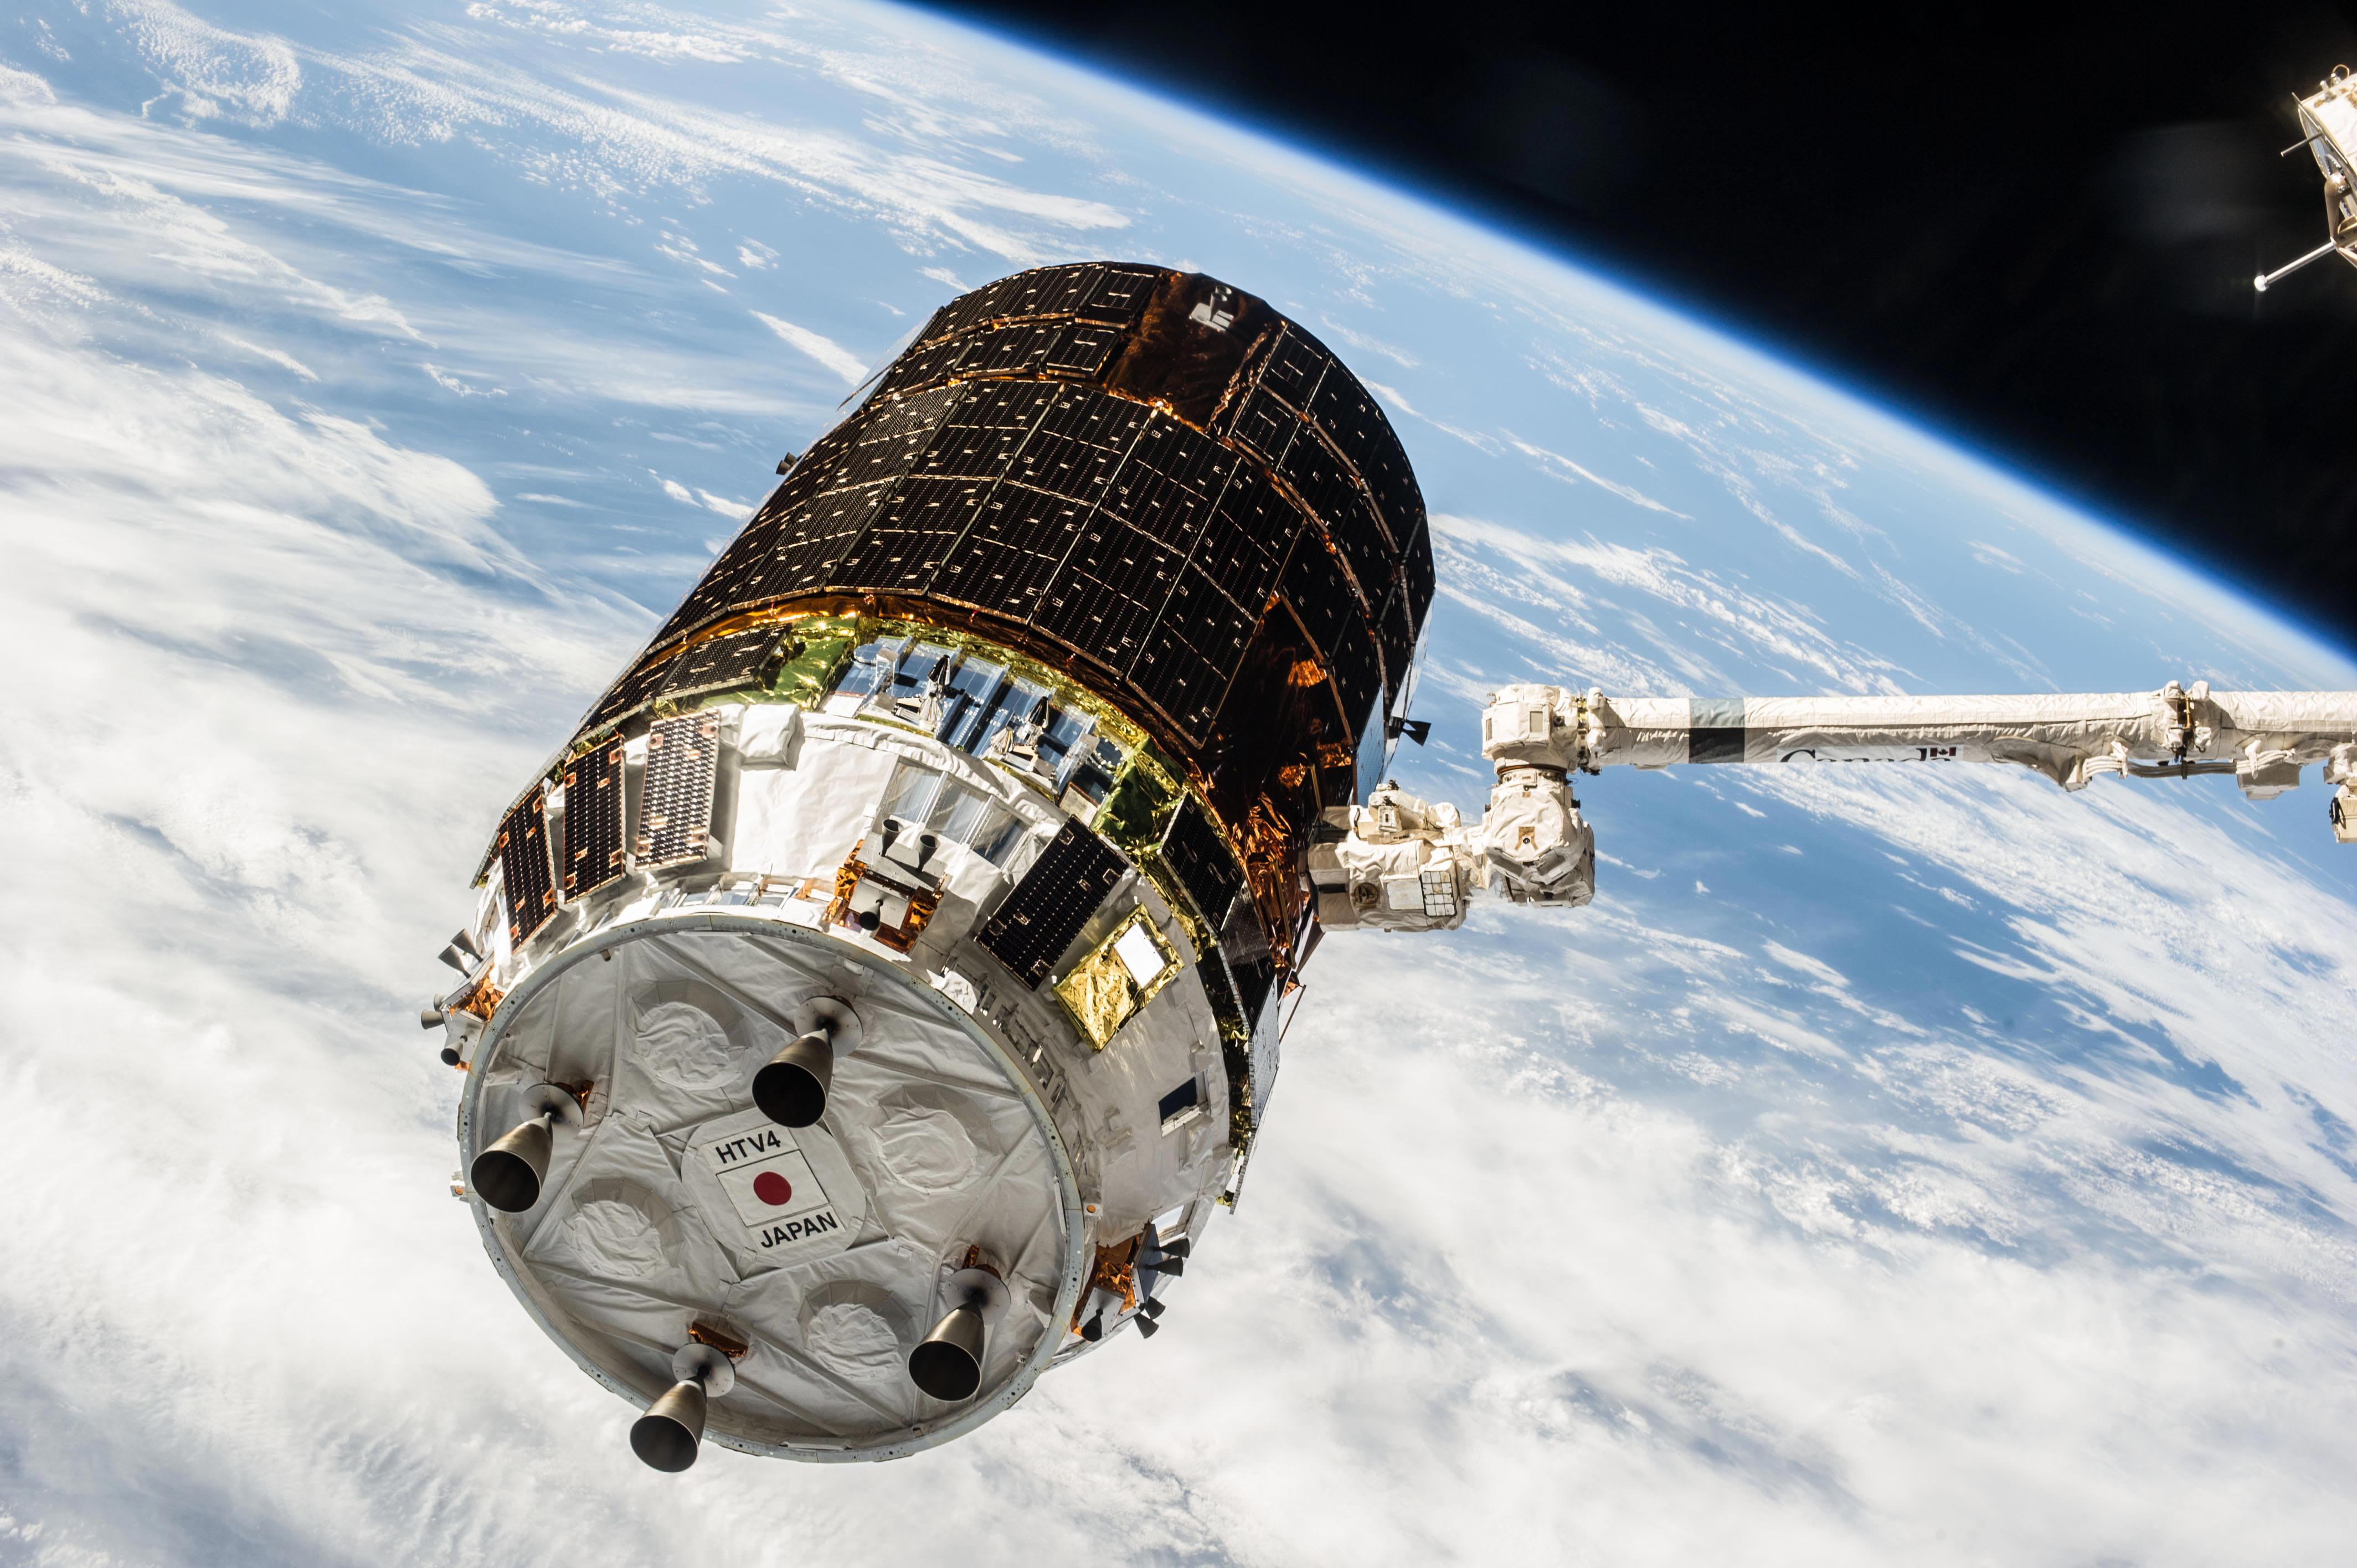
\includegraphics[width=\textwidth]{../img/grab5.jpg}};
        % \node<6> (img6) {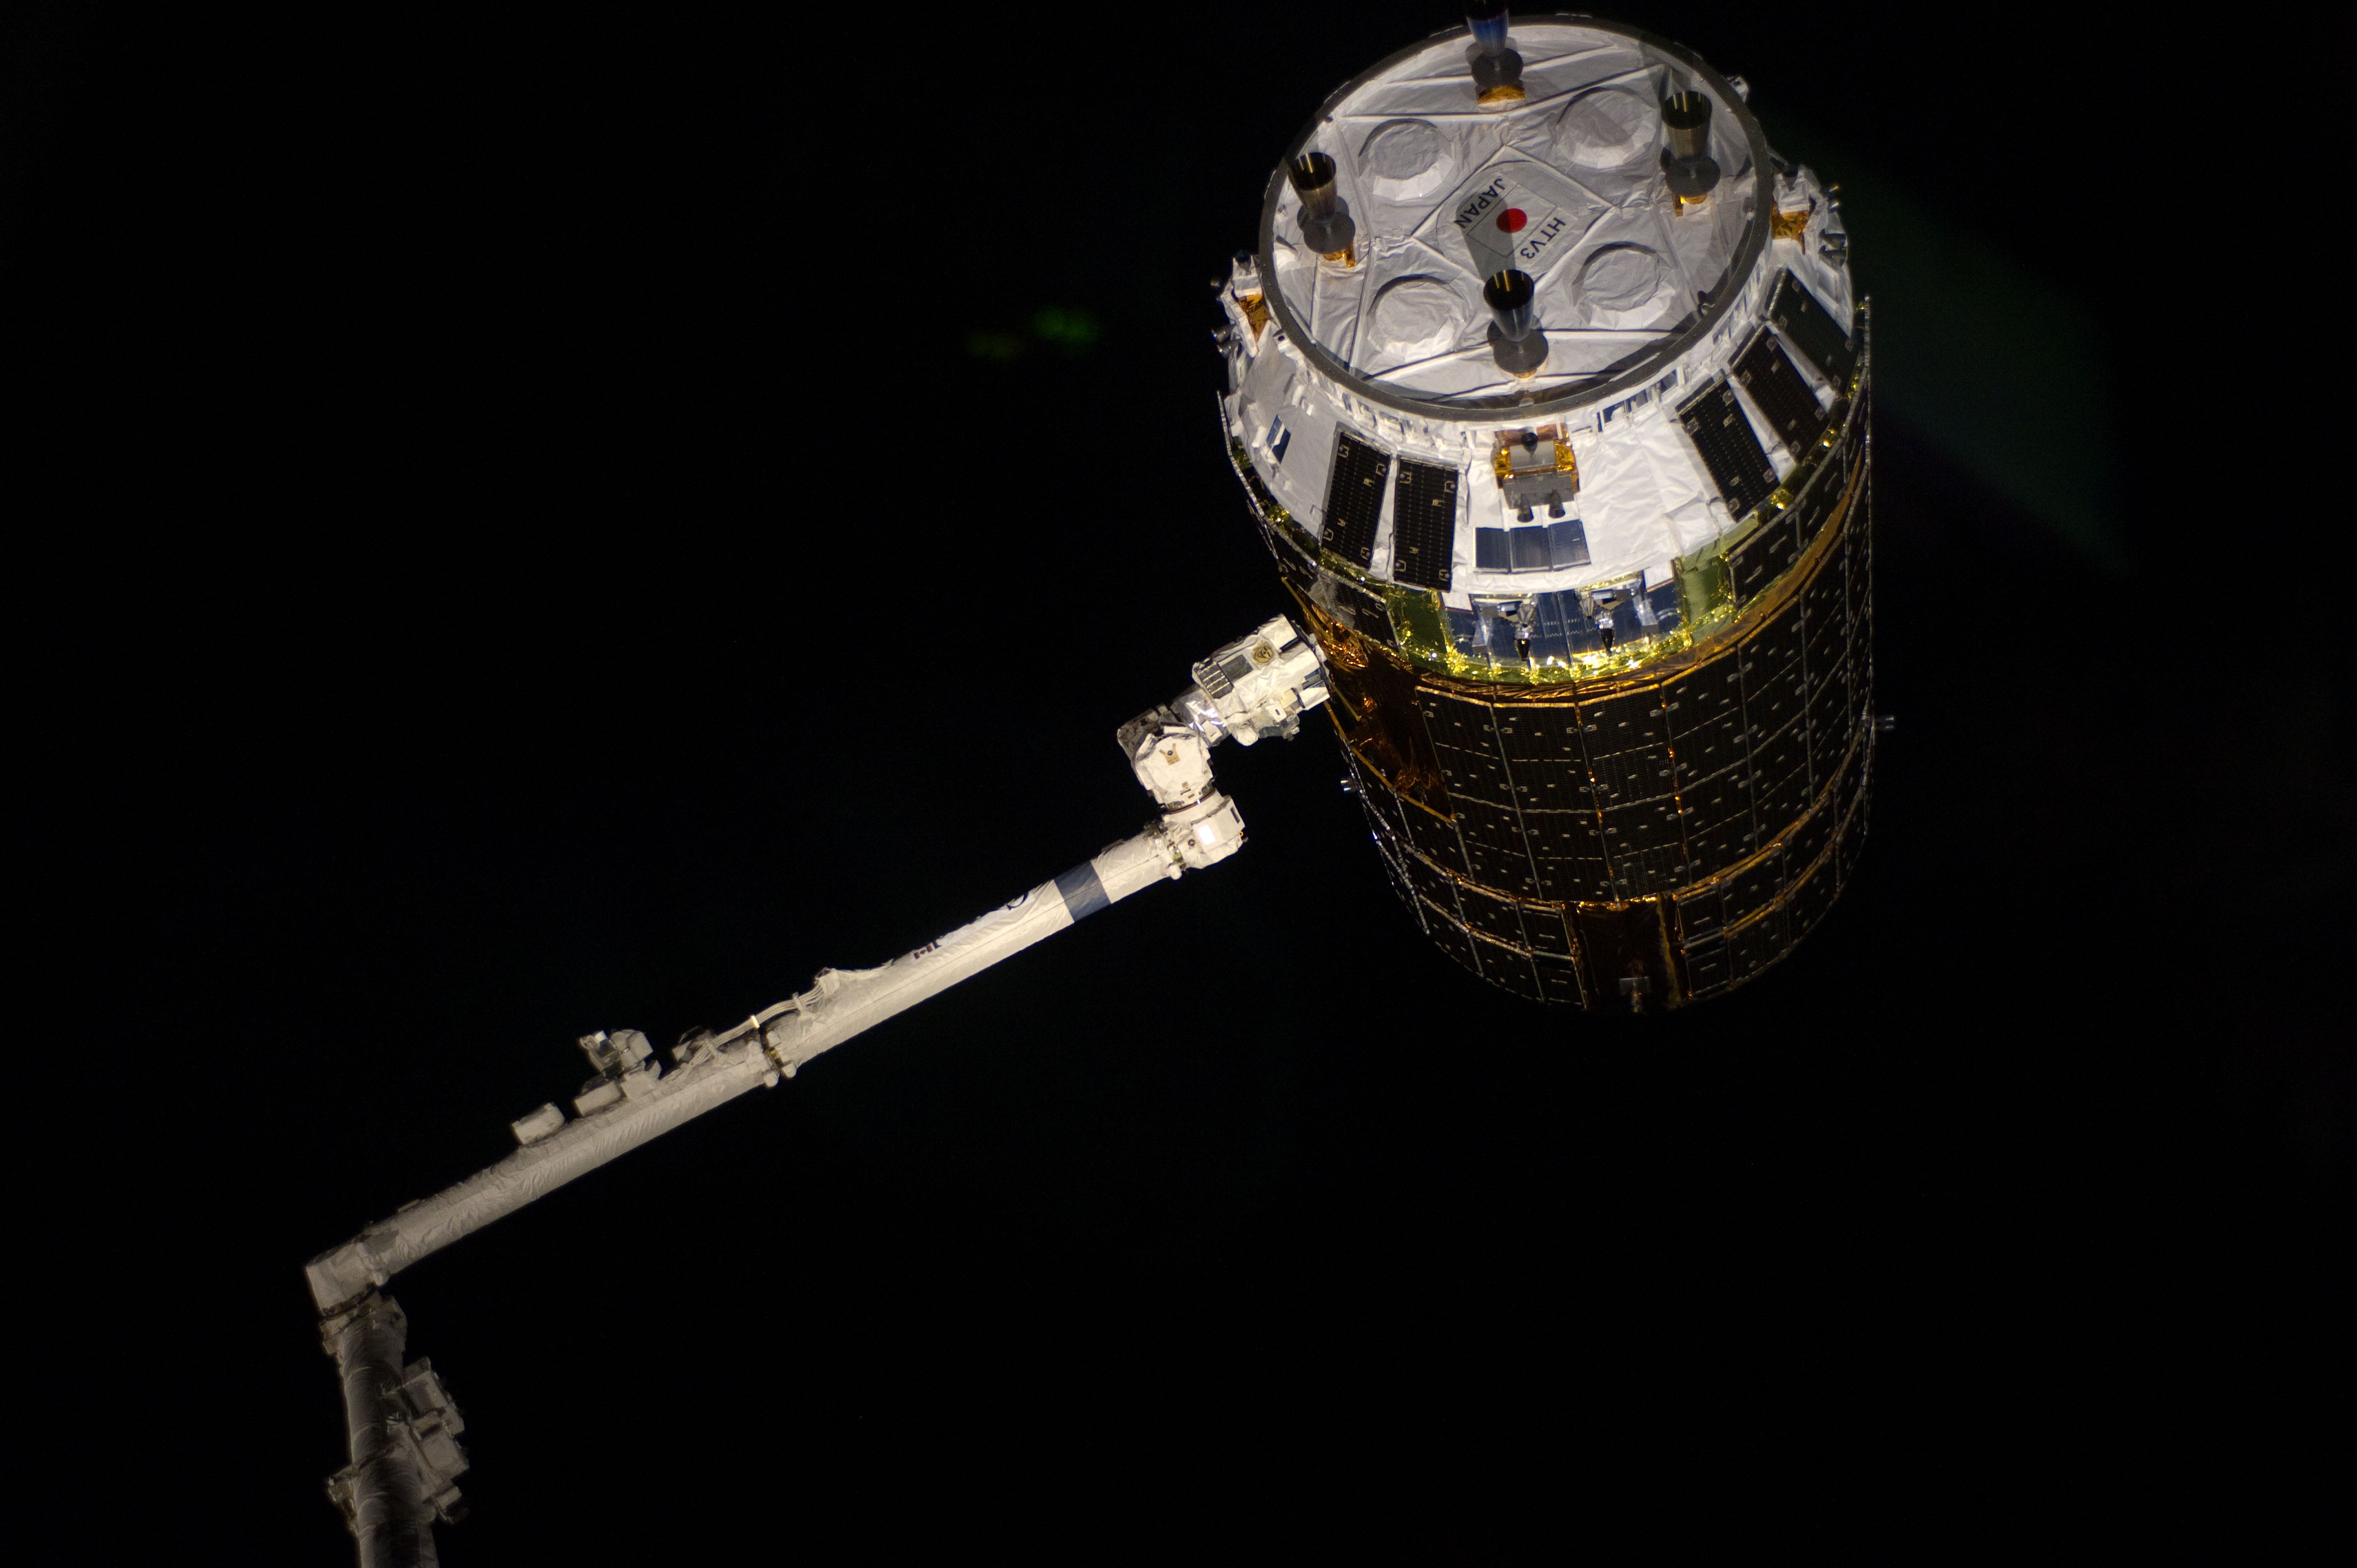
\includegraphics[width=\textwidth]{../img/grab6.jpg}};
        % \node<7> (img7) {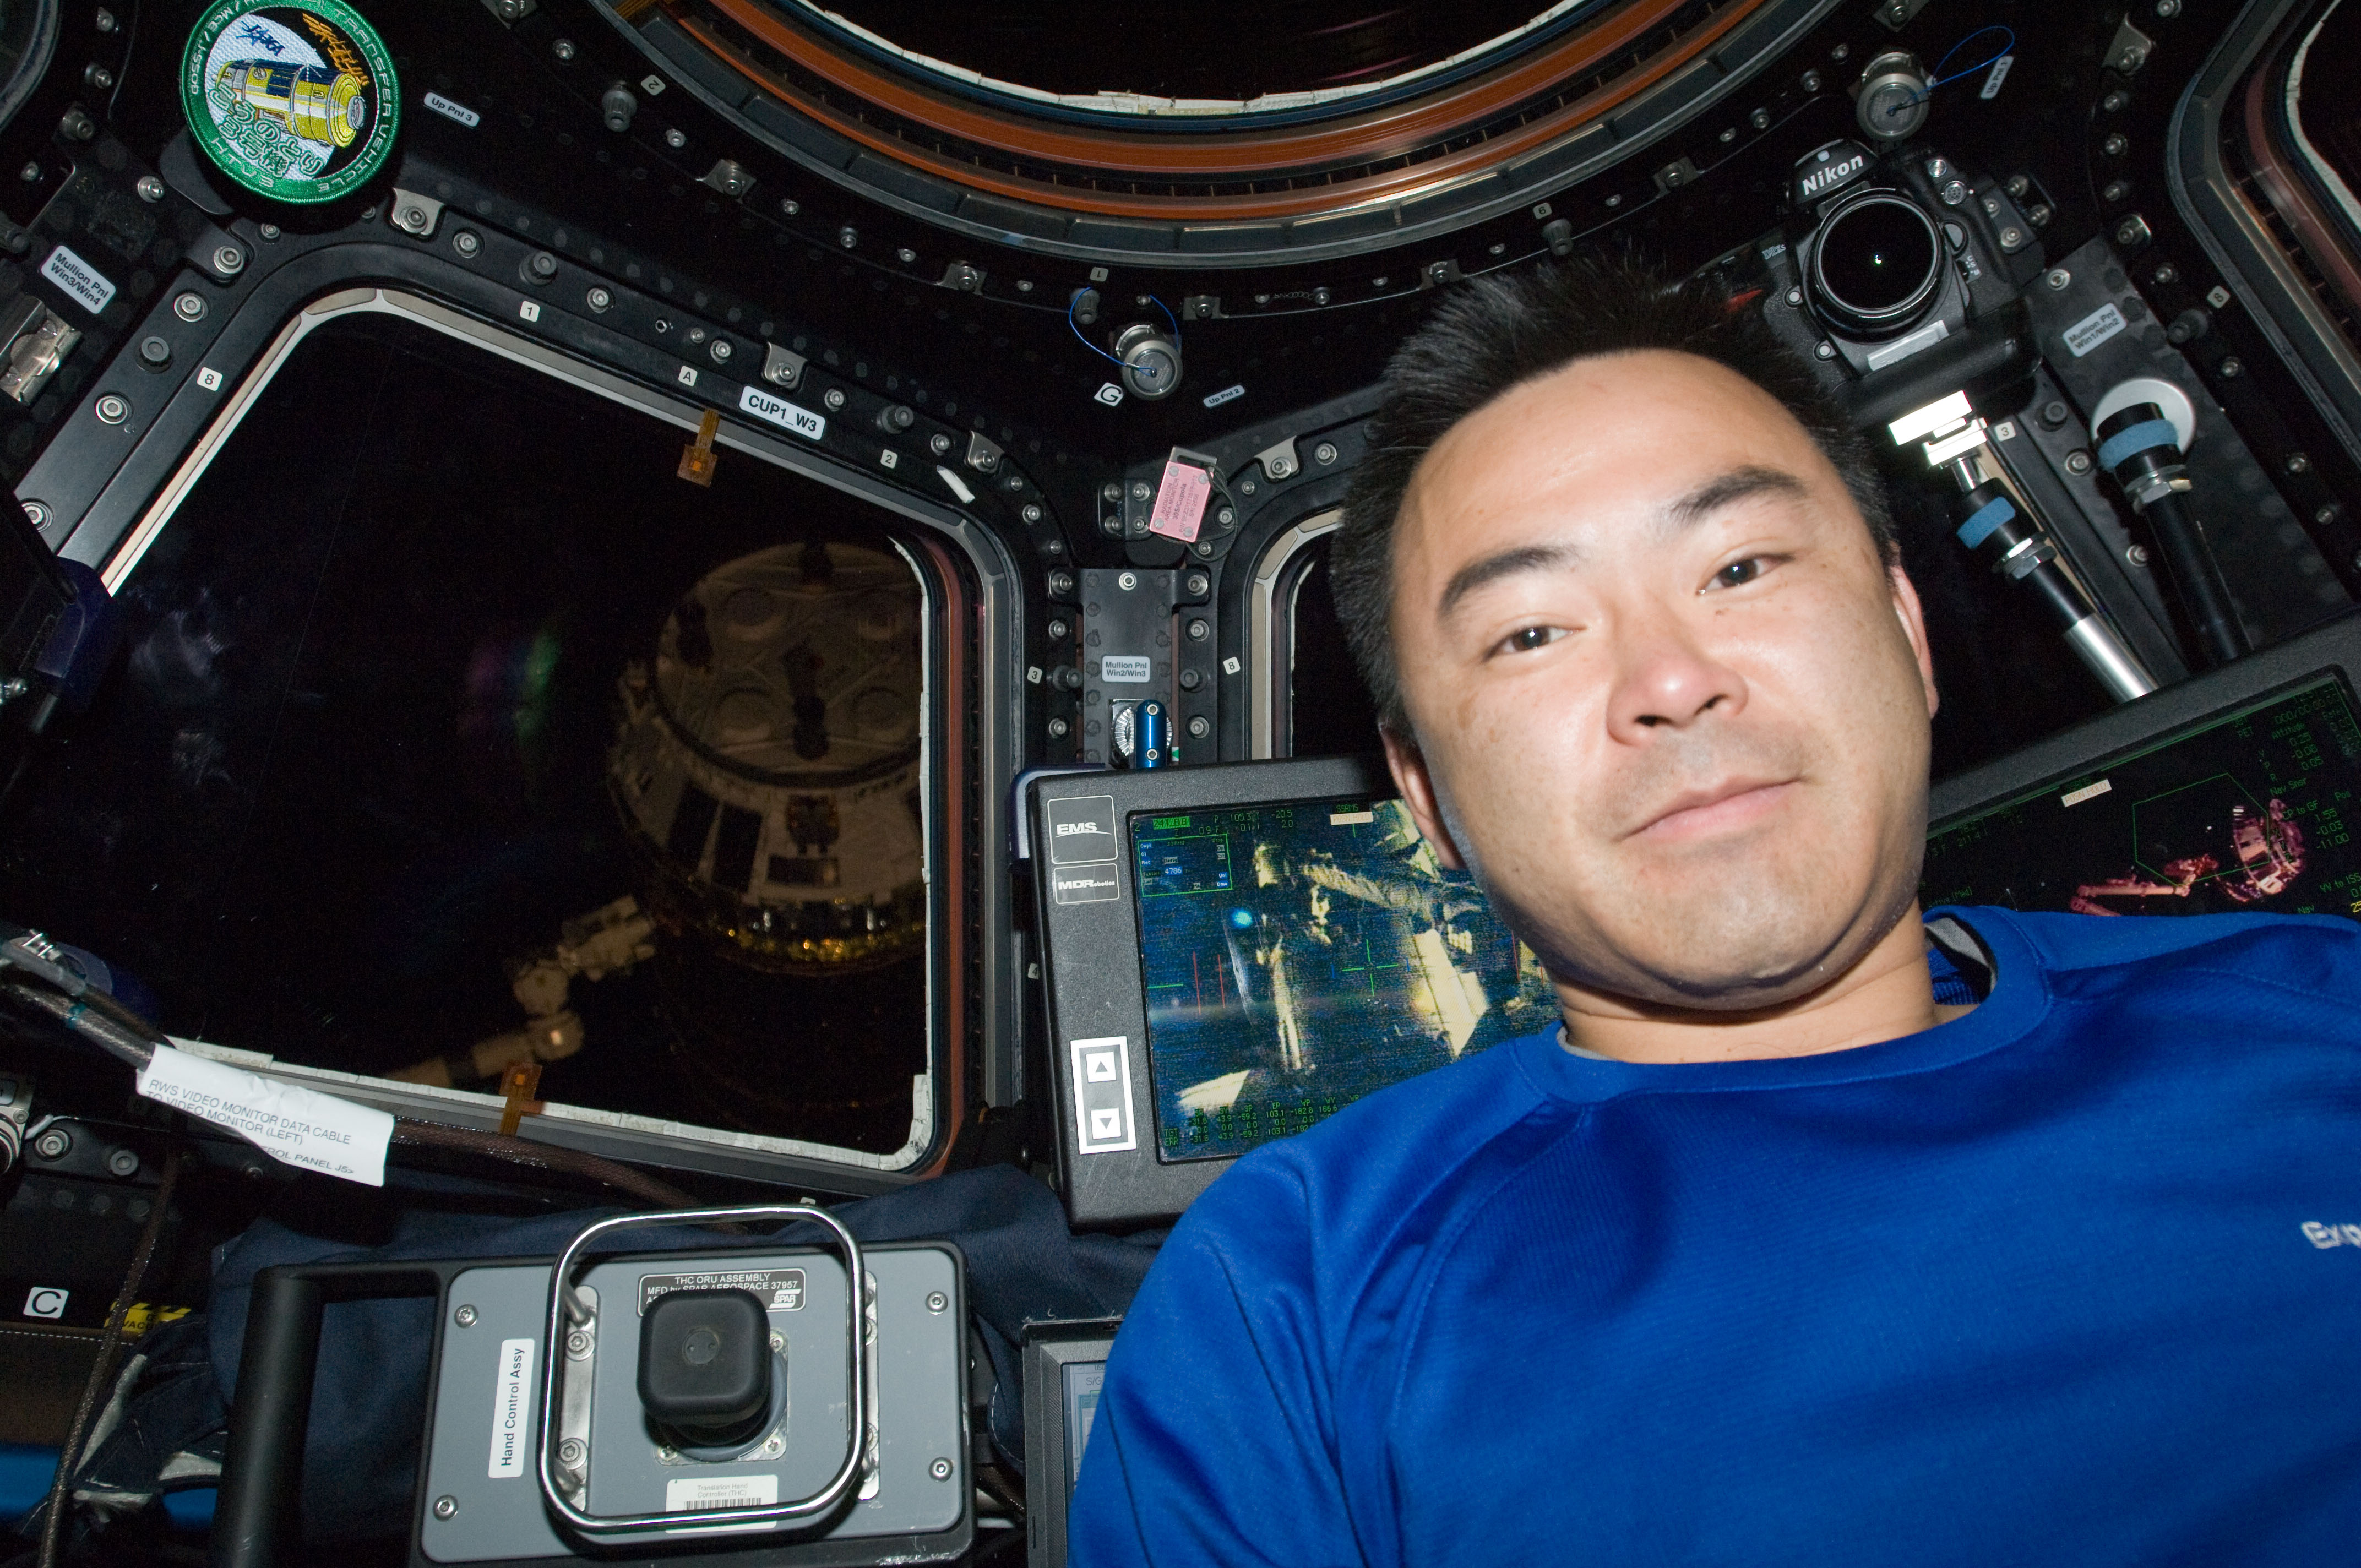
\includegraphics[width=\textwidth]{../img/grab7.jpg}};
      \end{tikzpicture}
    \end{column}
  \end{columns}
\end{frame}

\begin{frame}[fragile]{ROBoT Workstation}
\begin{figure}
  \begin{center}
    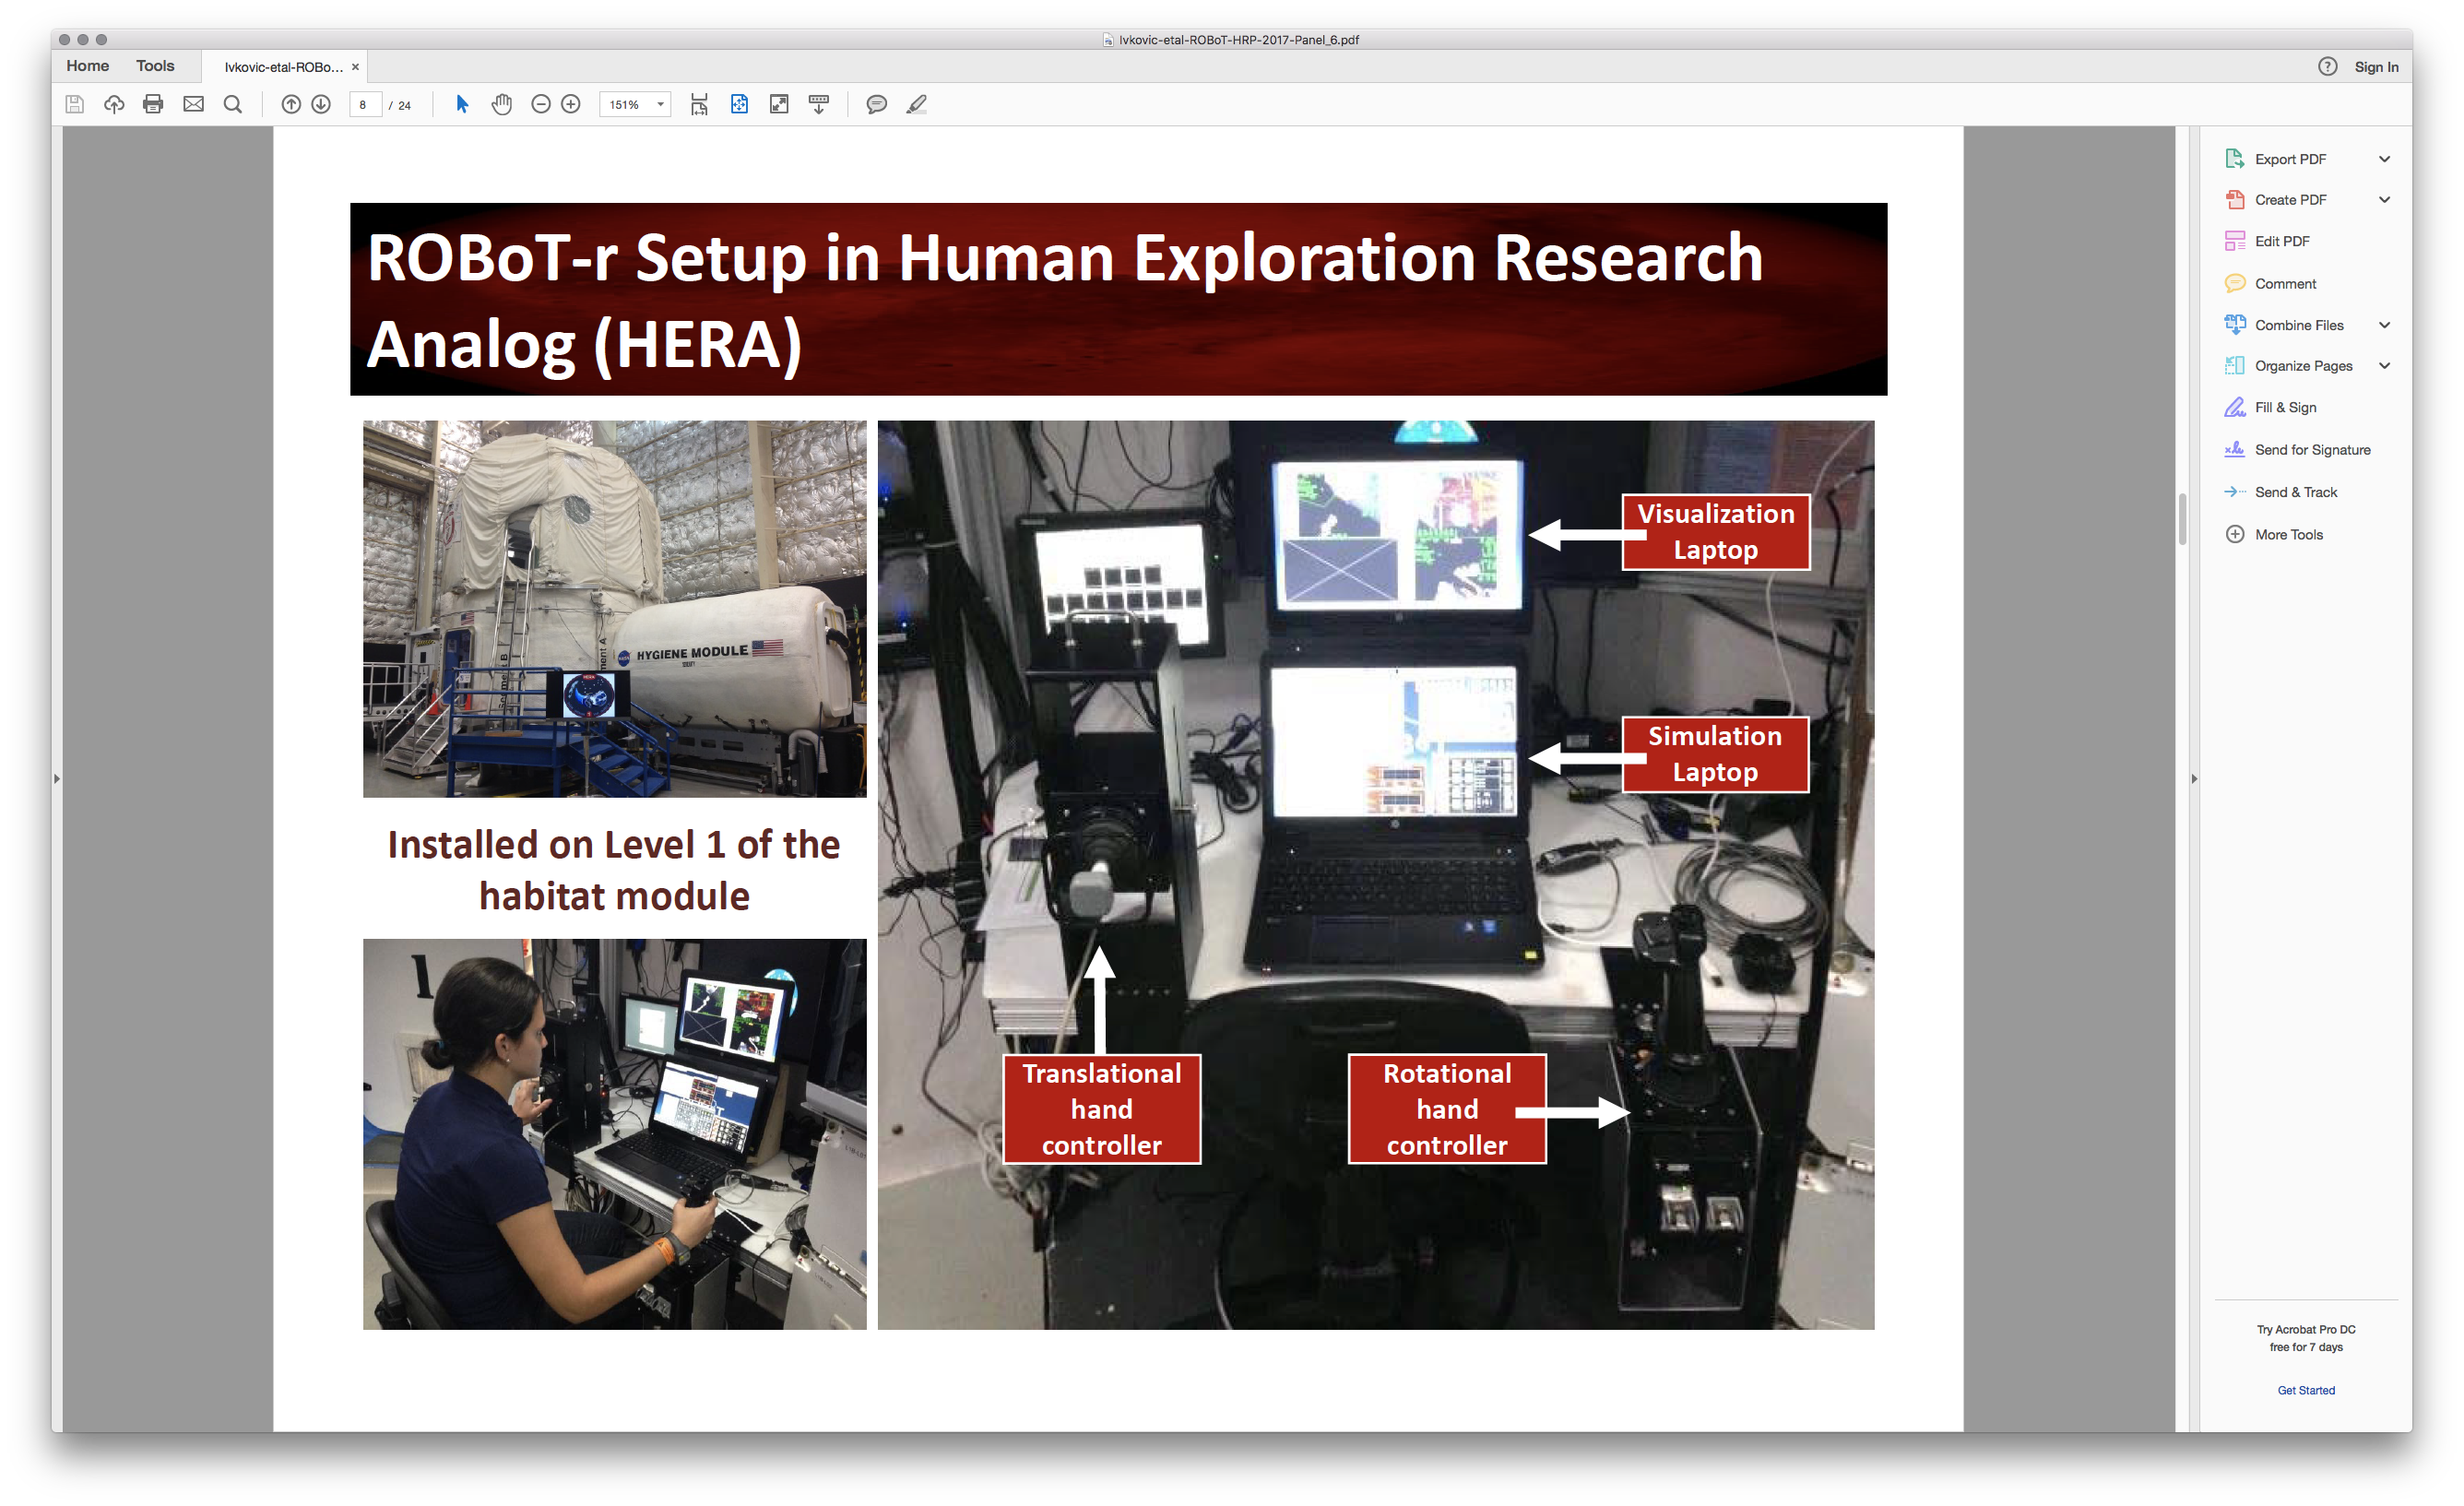
\includegraphics[trim={13cm 5cm 22cm 15.5cm},clip,width=\linewidth]{../img/Screen_Shot_2018-07-26_at_1.43.16_PM.png}
    % \caption{The Robotic On-board Trainer (ROBoT) station set up in the NASA HERA Analog, from~\cite{robottalk}.}
    % \label{figure:robotinhera}
  \end{center}
\end{figure}
\end{frame}

\begin{frame}[fragile]{ROBoT Visualization}
\begin{figure}
  \begin{center}
    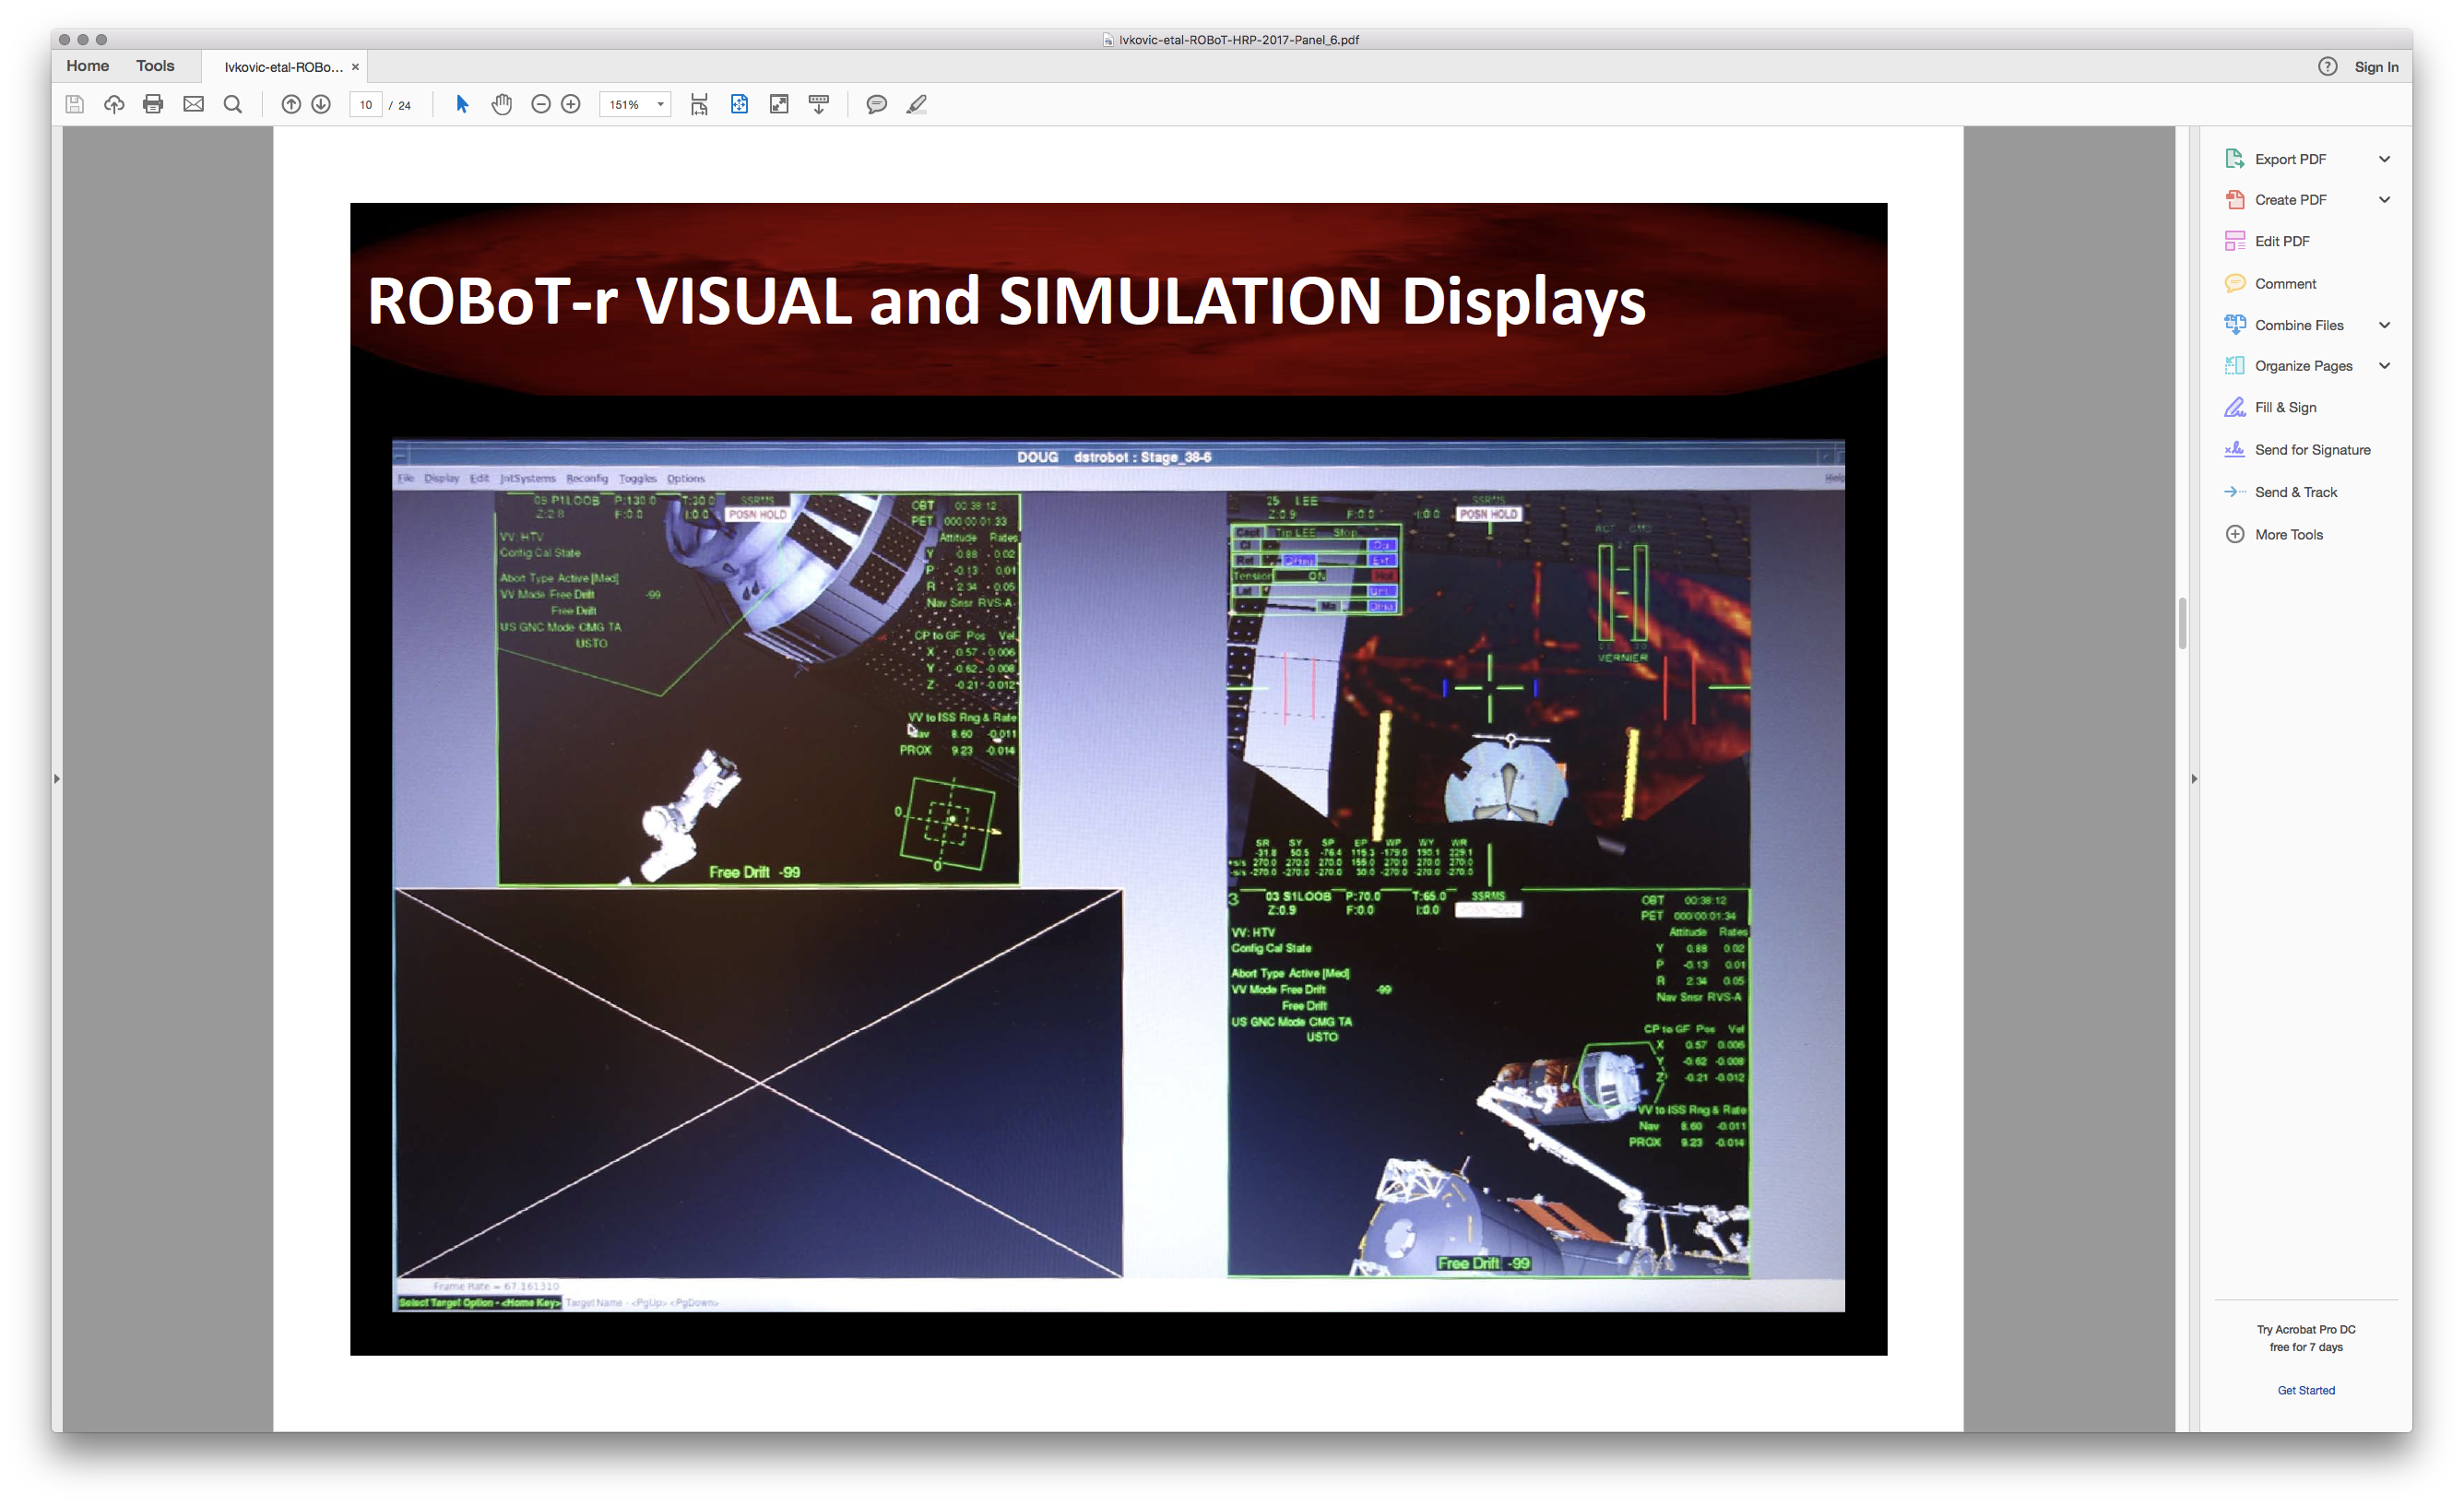
\includegraphics[trim={13cm 5cm 22cm 15.5cm},clip,width=\linewidth]{../img/Screen_Shot_2018-07-26_at_1.43.02_PM.png}
    % \caption{ROBoT visualization laptop, showing four camera views.}
    % \label{}
  \end{center}
\end{figure}
\end{frame}

% \begin{frame}[fragile]{ROBoT End Effector View}
% \begin{figure}
%   \begin{center}
%     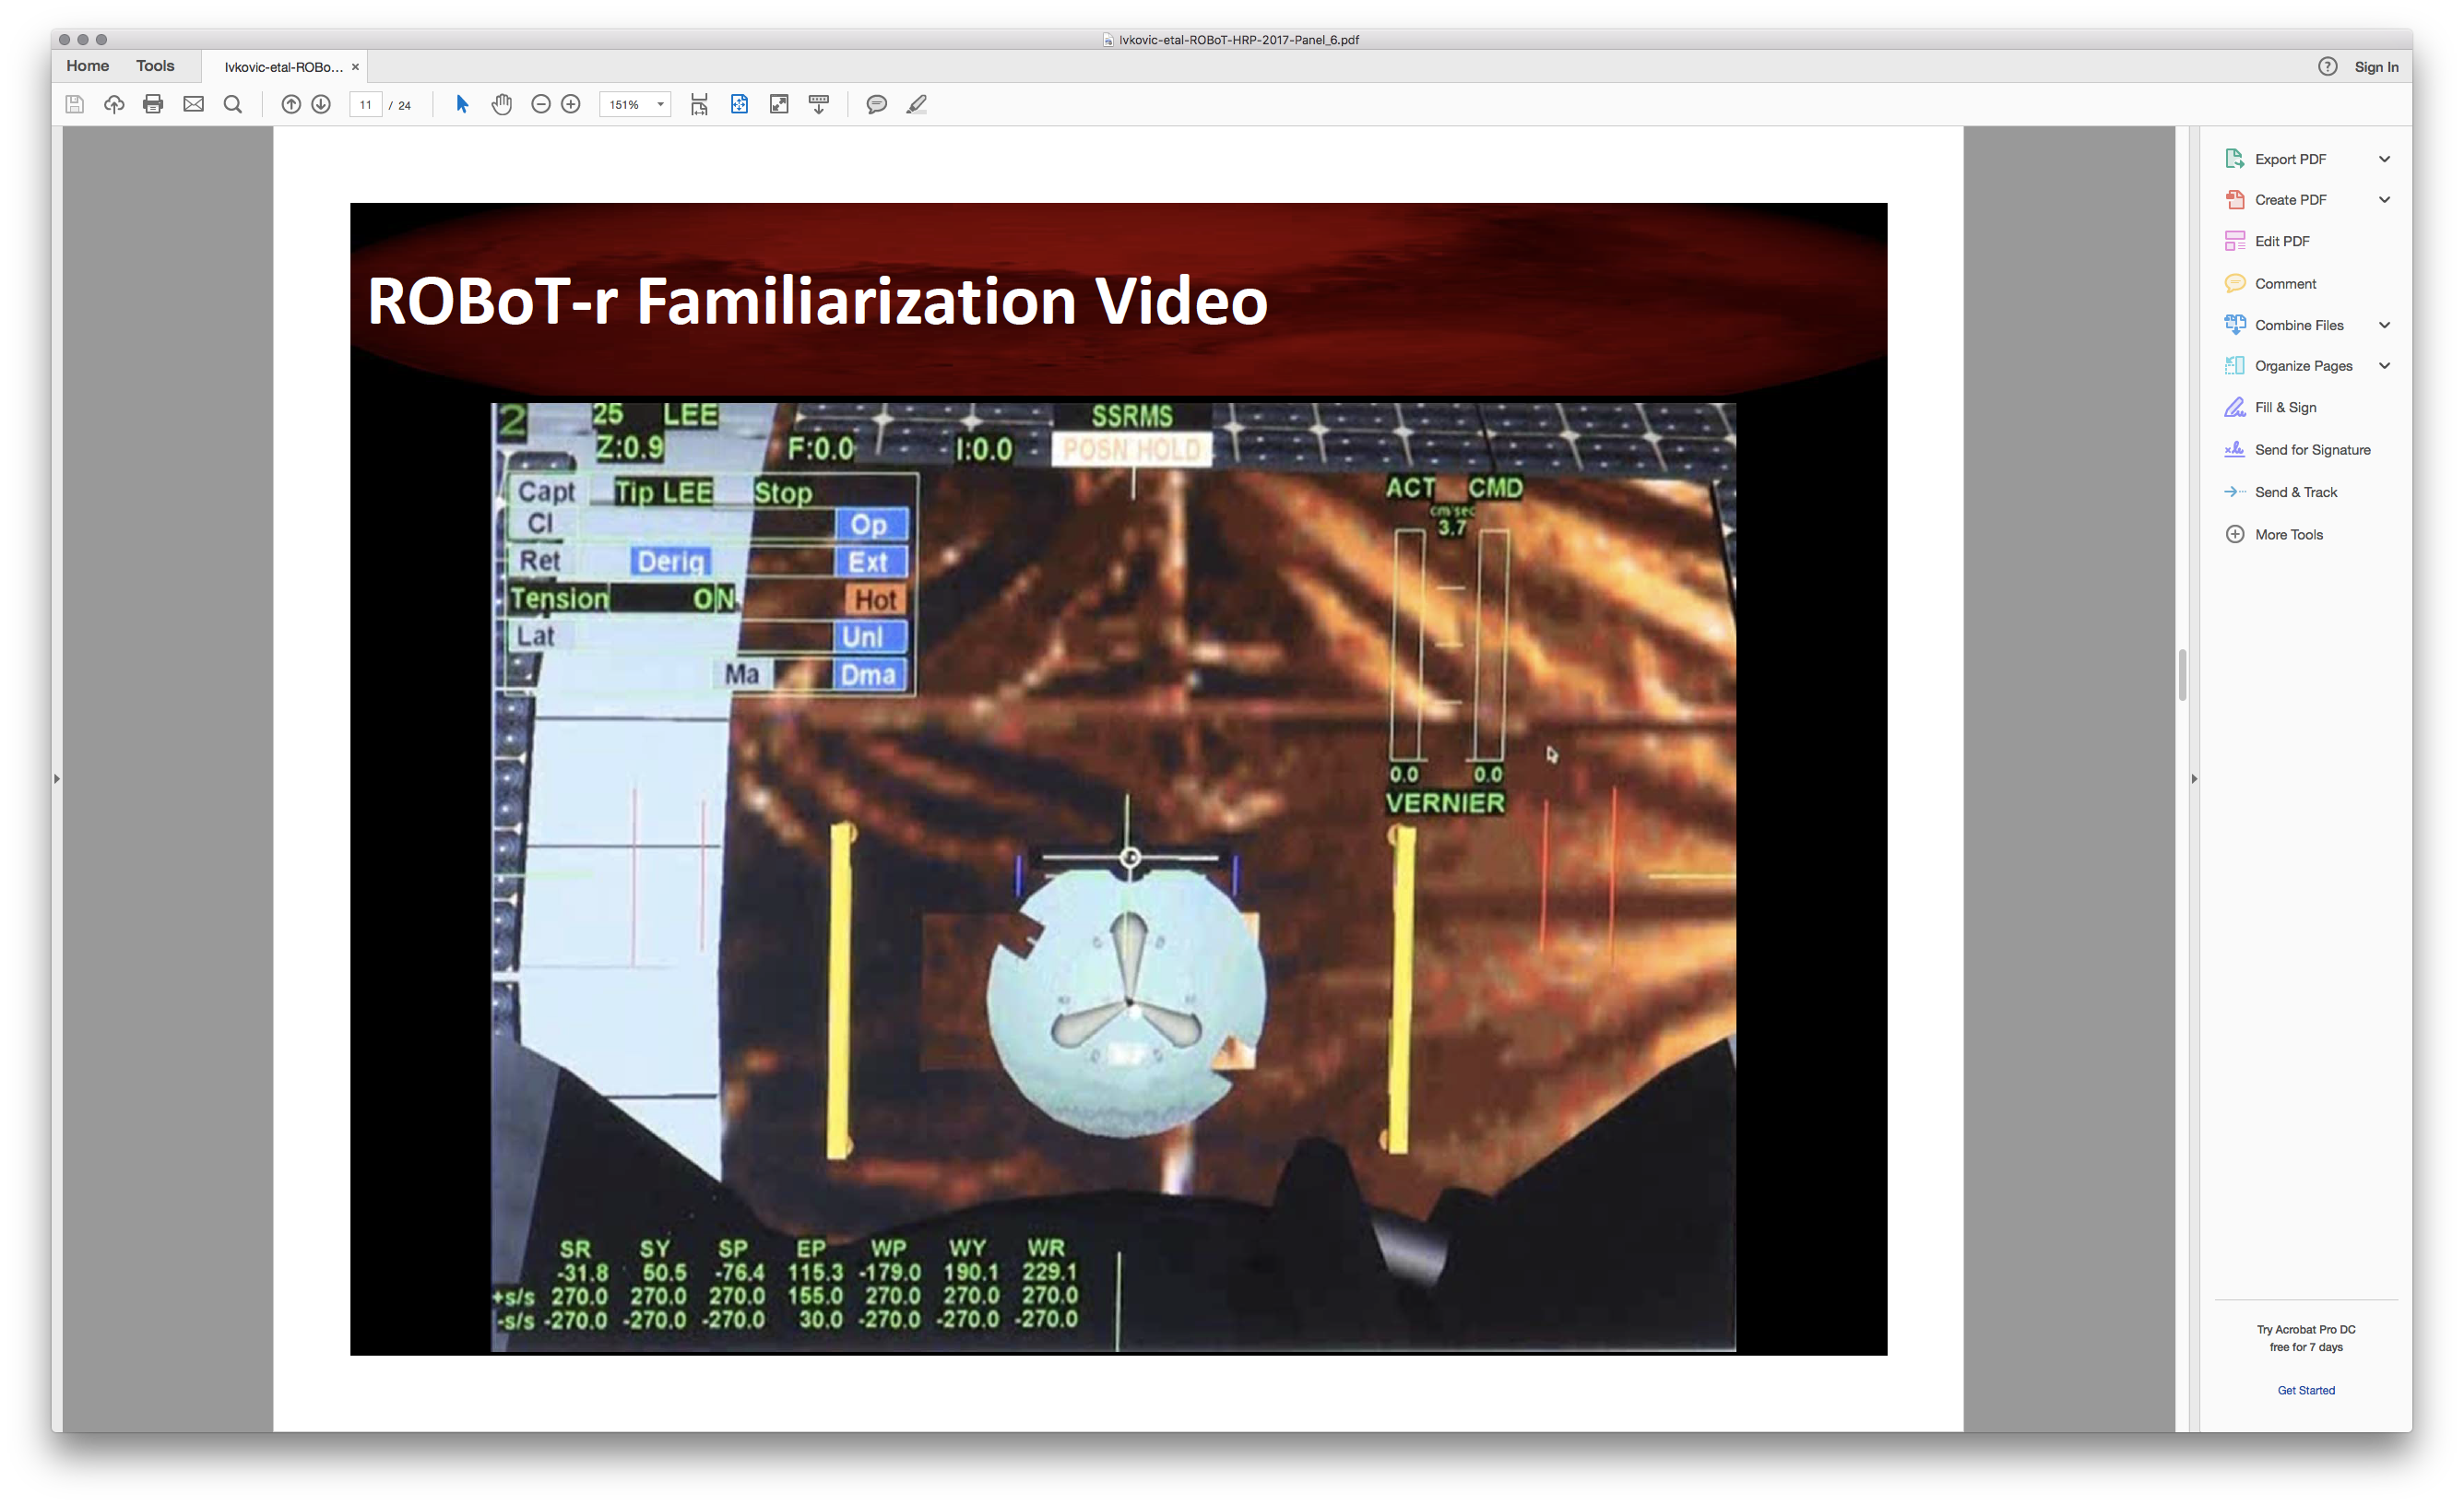
\includegraphics[trim={13cm 5cm 22cm 15.5cm},clip,width=\linewidth]{../img/Screen_Shot_2018-07-26_at_1.43.05_PM.png}
%     % \caption{The camera attached to the end effector of the robotic arm, showing the grapple fixture.}
%     % \label{}
%   \end{center}
% \end{figure}
% \end{frame}

\begin{frame}[fragile]{ROBoT Performance Reports}
\begin{figure}
  \begin{center}
    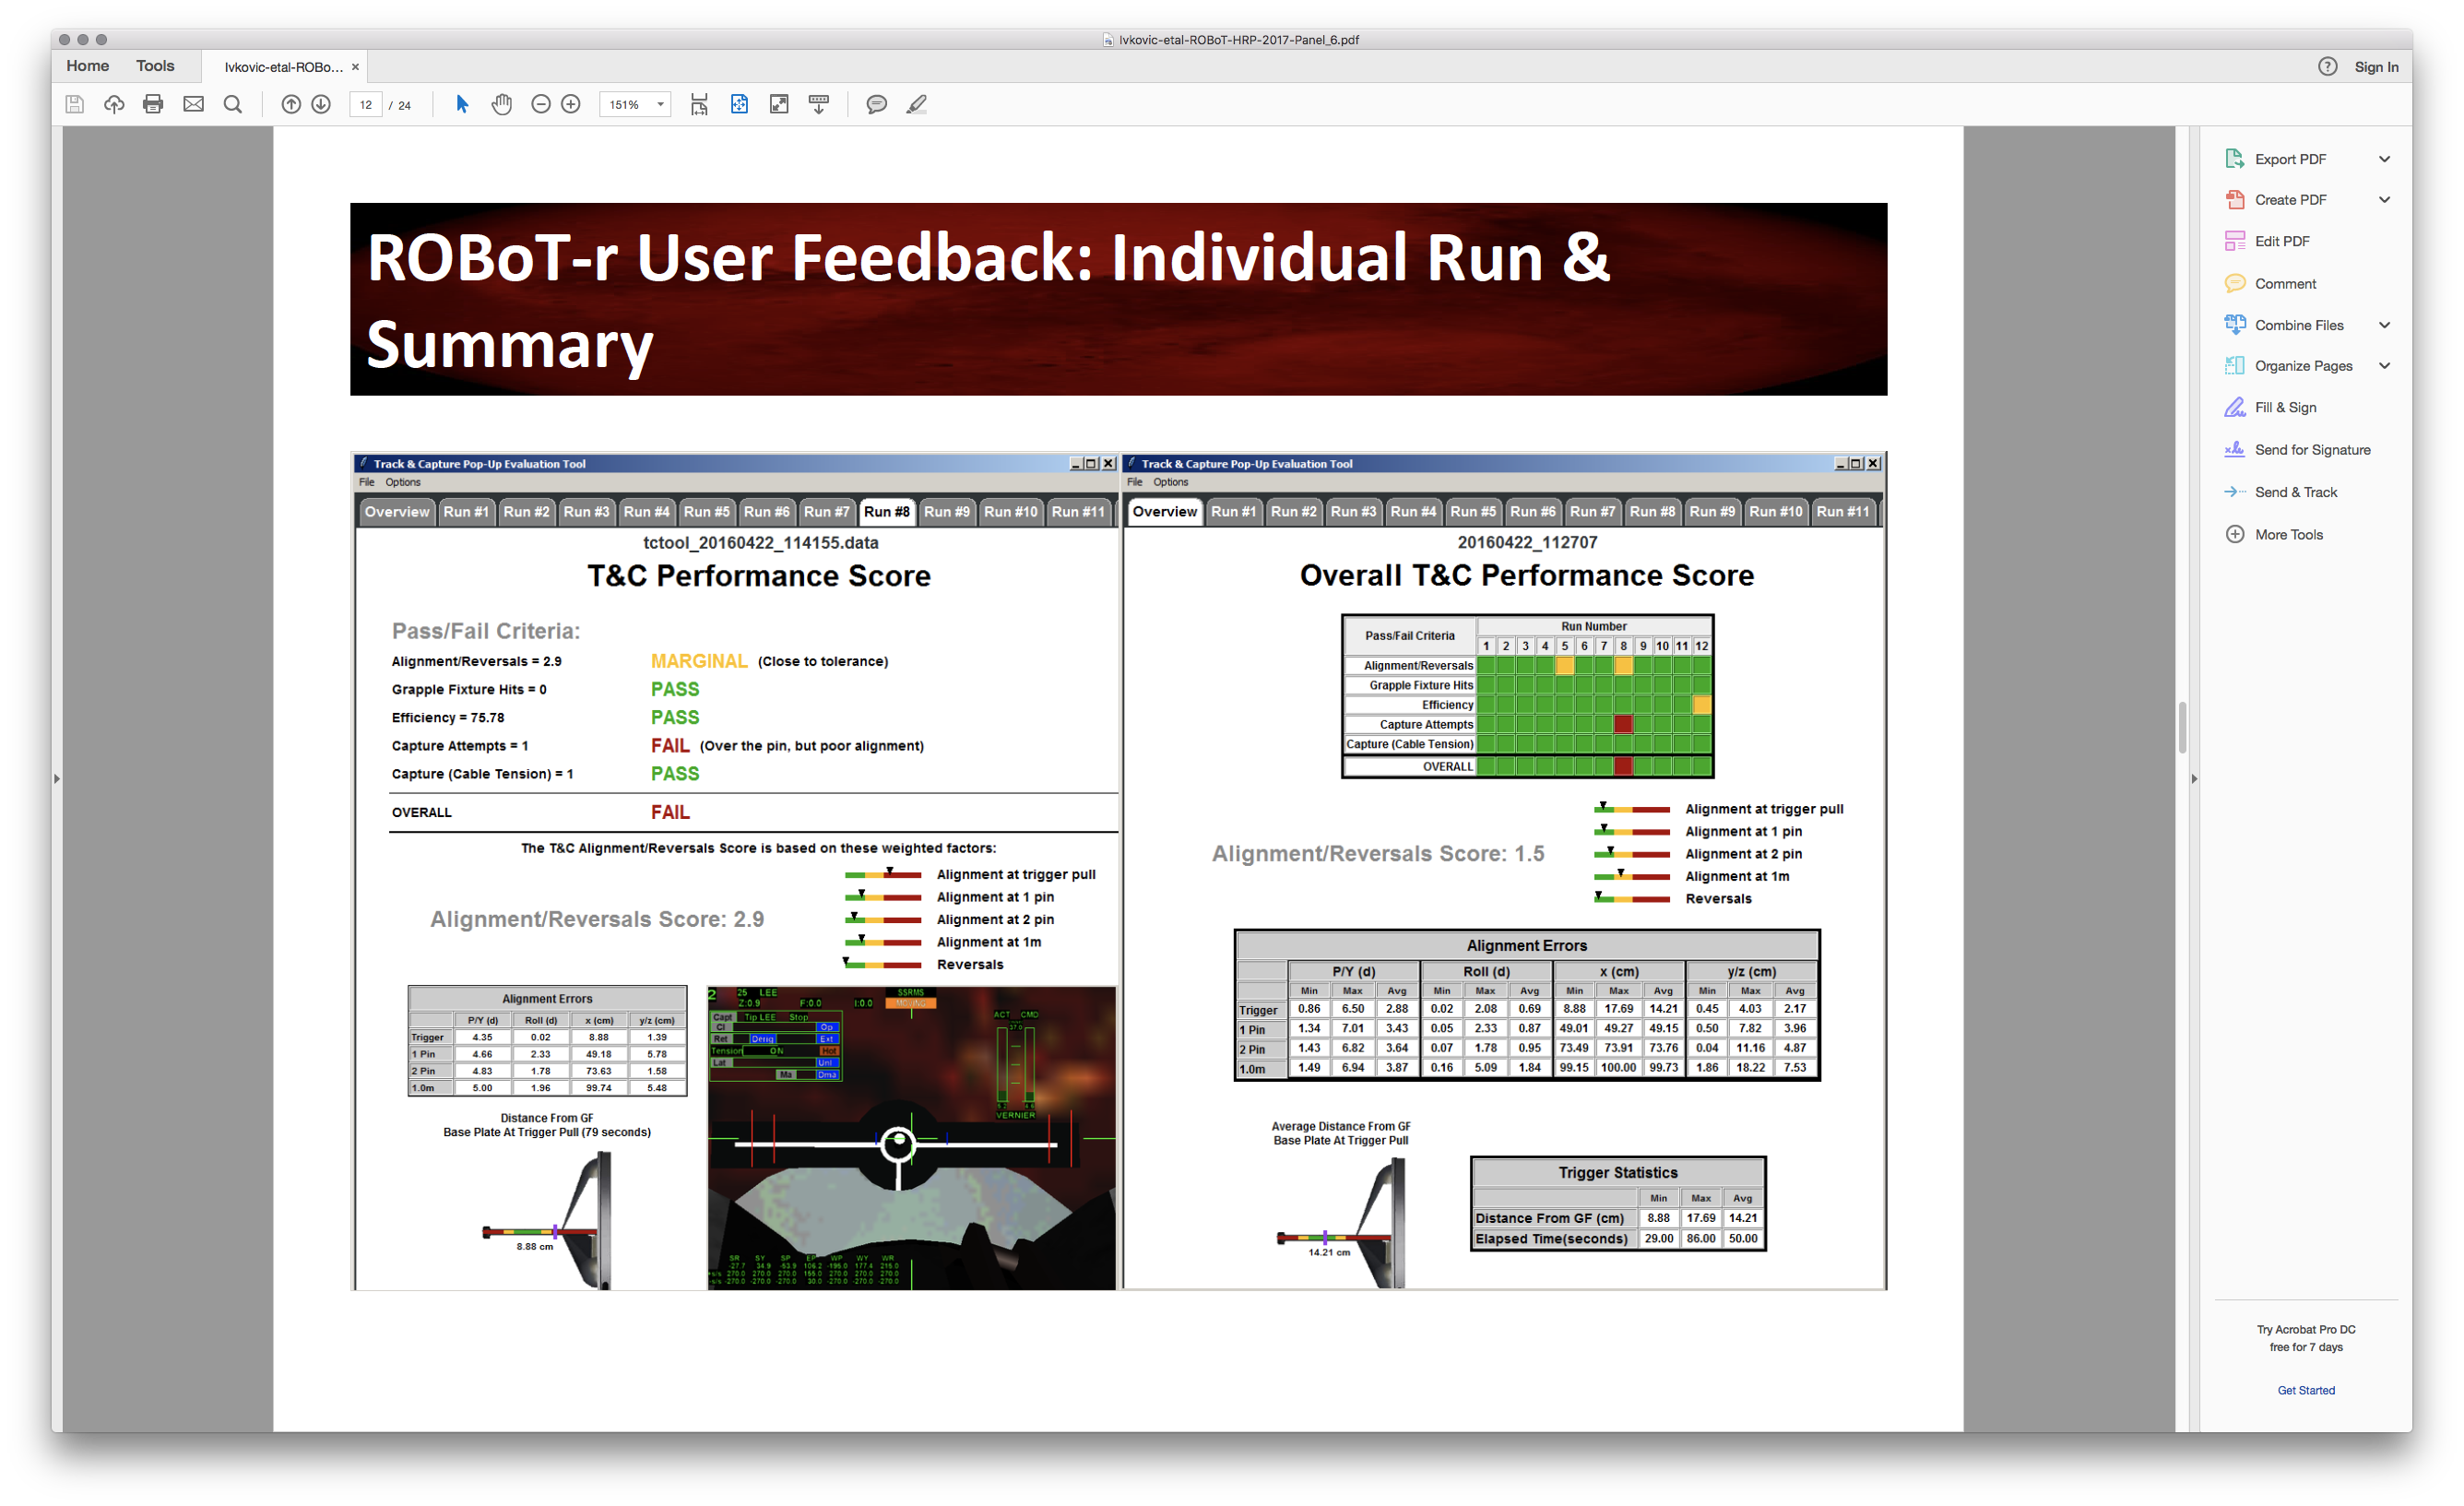
\includegraphics[trim={13cm 5cm 22cm 15.5cm},clip,width=\linewidth]{../img/Screen_Shot_2018-07-26_at_1.43.07_PM.png}
    % \caption{Example performance score report shown to the user after each trial.}
    % \label{}
  \end{center}
\end{figure}
\end{frame}

% \begin{frame}[fragile]{ROBoT Data Output}
% \begin{figure}
%   \begin{center}
%     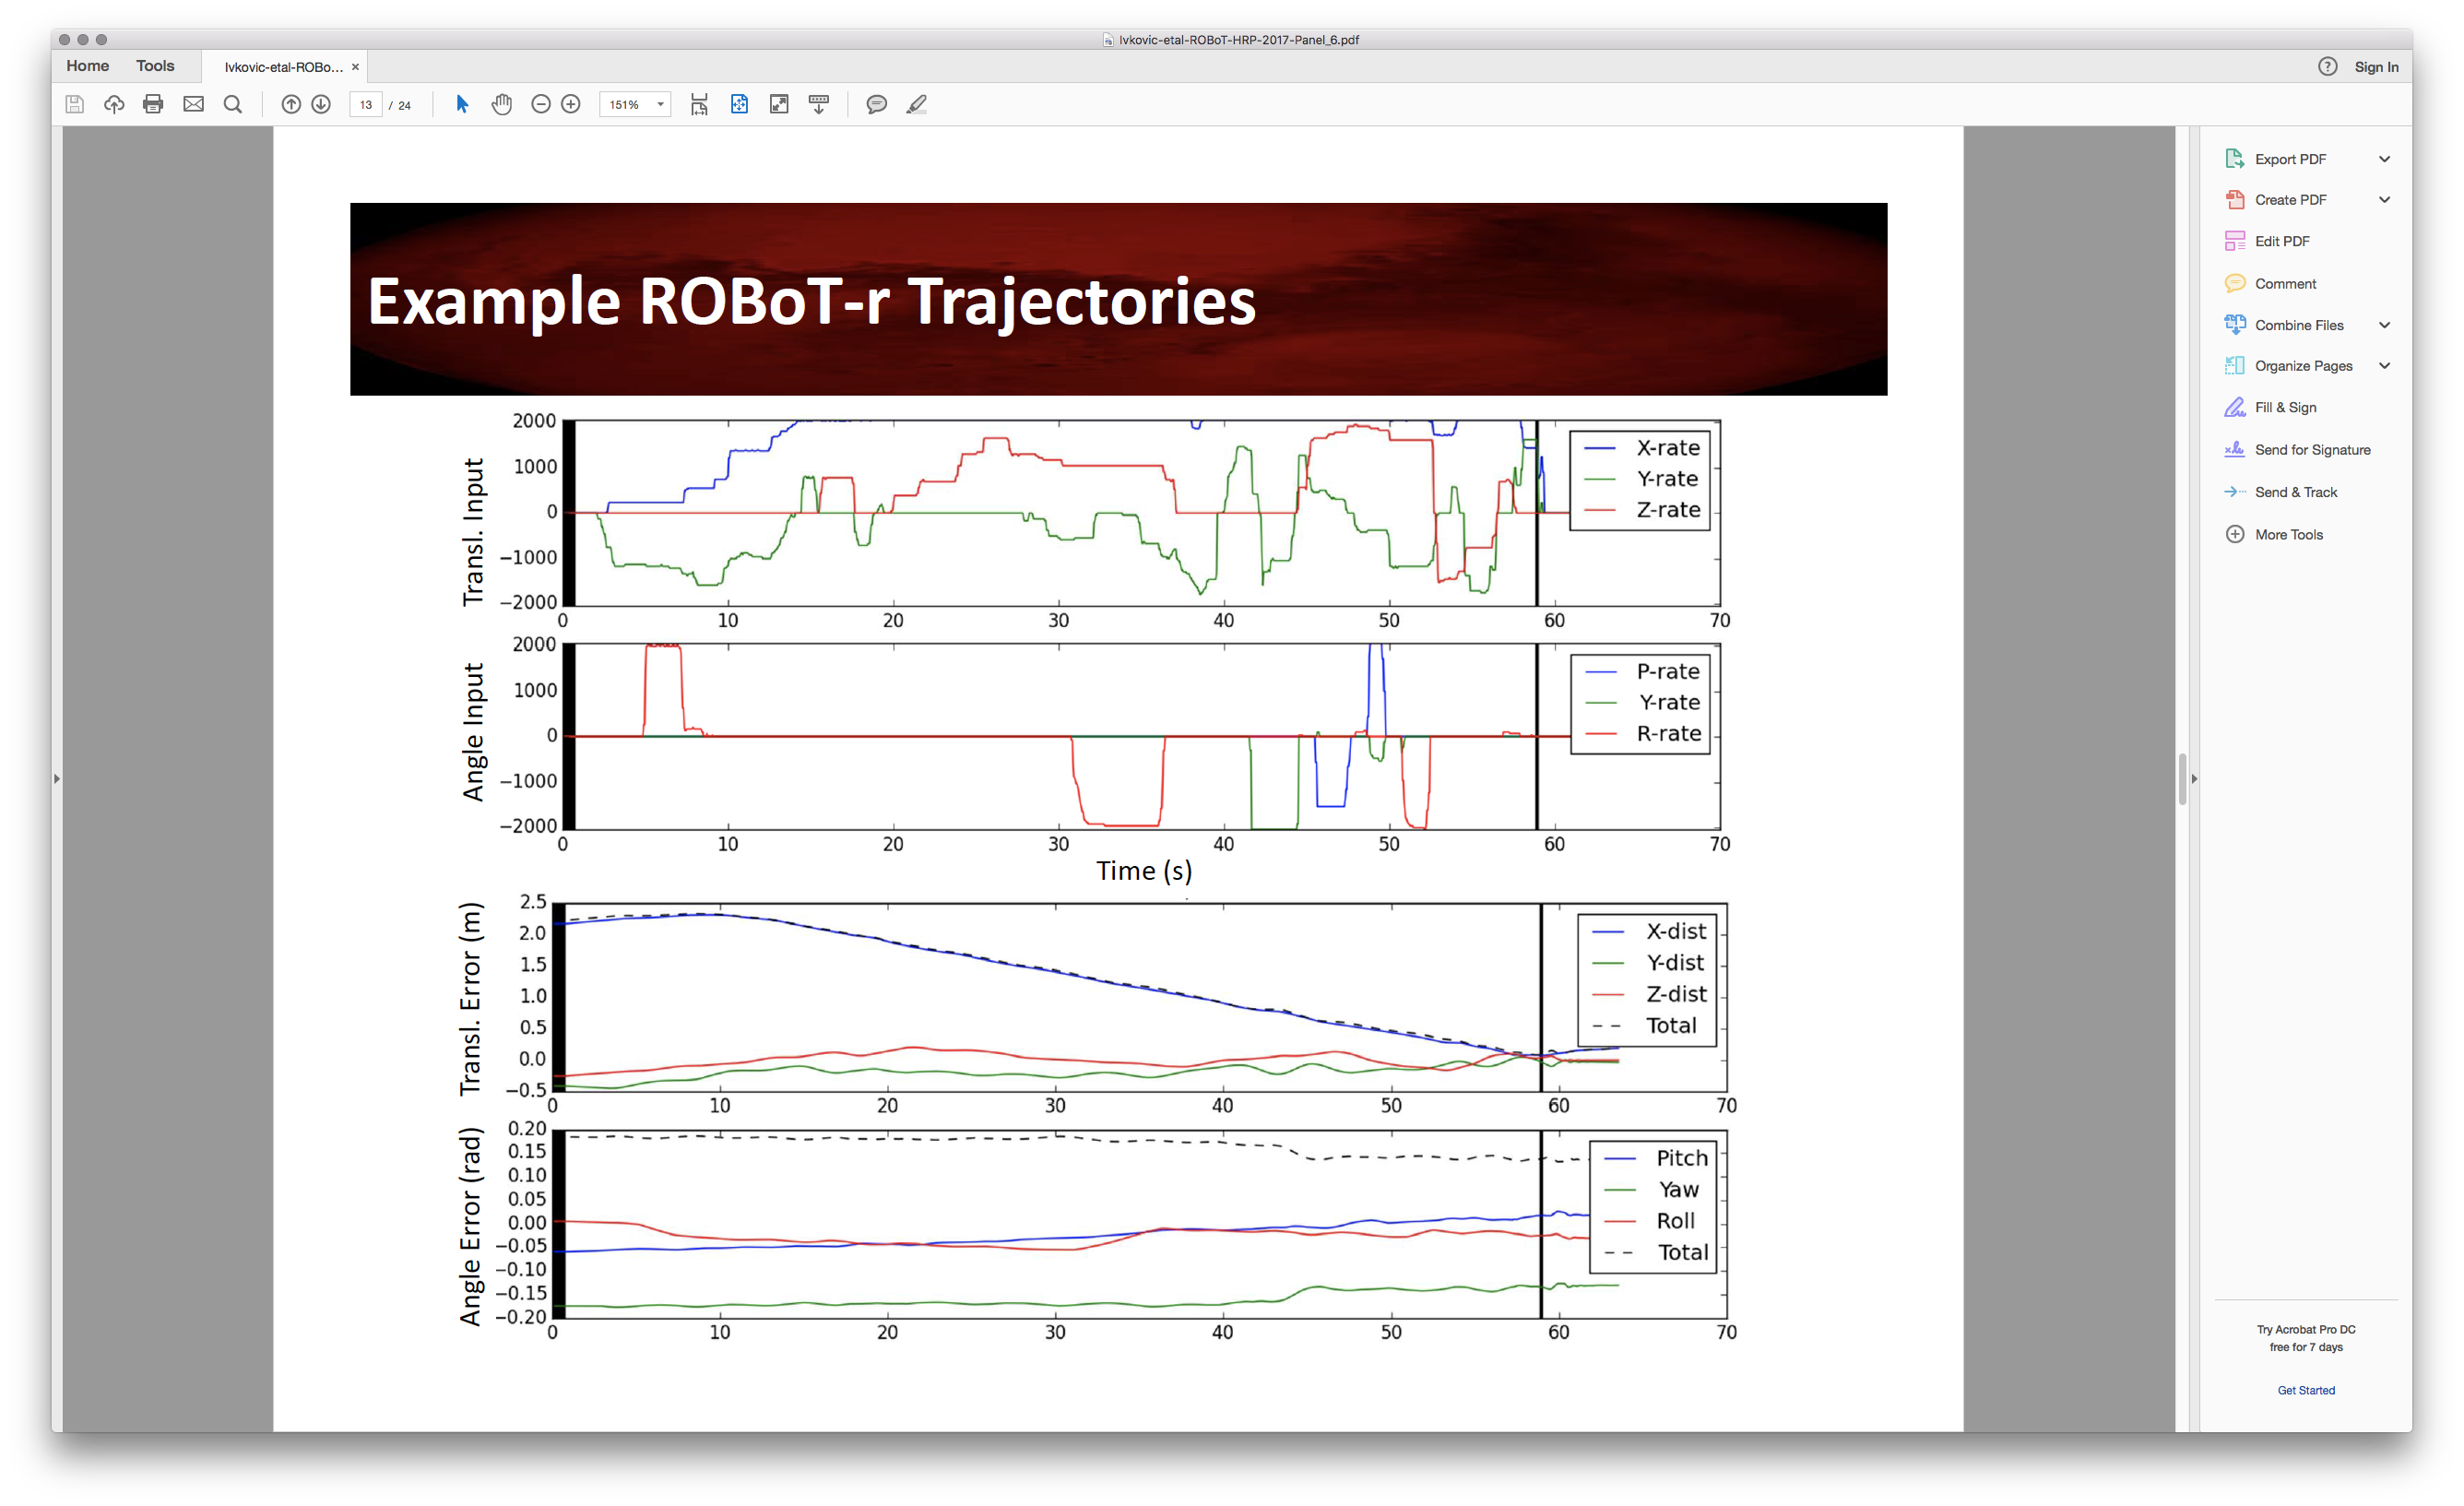
\includegraphics[trim={13cm 5cm 22cm 15.5cm},clip,width=\linewidth]{../img/Screen_Shot_2018-07-26_at_1.43.10_PM.png}
%     % \caption{The hand controller inputs and position and angular errors are also logged throughout the trial.}
%     % \label{}
%   \end{center}
% \end{figure}
% \end{frame}

\begin{frame}[fragile]{Experiment Two}
  \begin{itemize}
    \setlength\itemsep{1em}
    \item Only terminal feedback is currently available without a trainer
    \item Terminal feedback is ineffective for complex tasks
    \item Provide feedback concurrently with task execution
  \end{itemize}
\end{frame}

\begin{frame}[fragile]{ROBoT Treatment Group}
\begin{figure}
  \begin{center}

  \begin{tikzpicture}
    \node<1-> (img1) {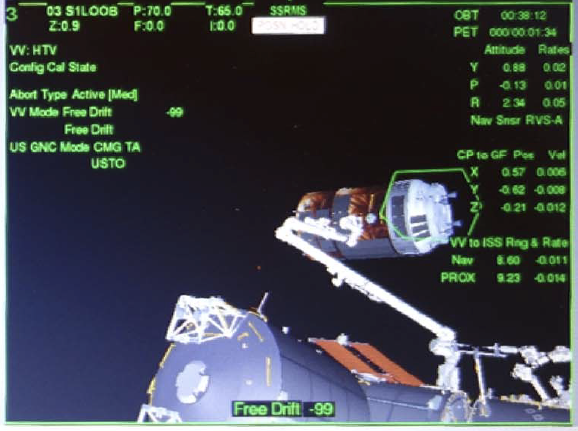
\includegraphics[width=\textwidth]{../img/robot_edit.png}};
    % \draw<2-> (0,0) ellipse (2cm and 1cm);
    \draw<2-> [red,ultra thick] (4,1.5) ellipse (1cm and 2cm);
  \end{tikzpicture}

  \end{center}
\end{figure}
\end{frame}

\begin{frame}[fragile]{Experiment Two Flowchart}
  \begin{center}
    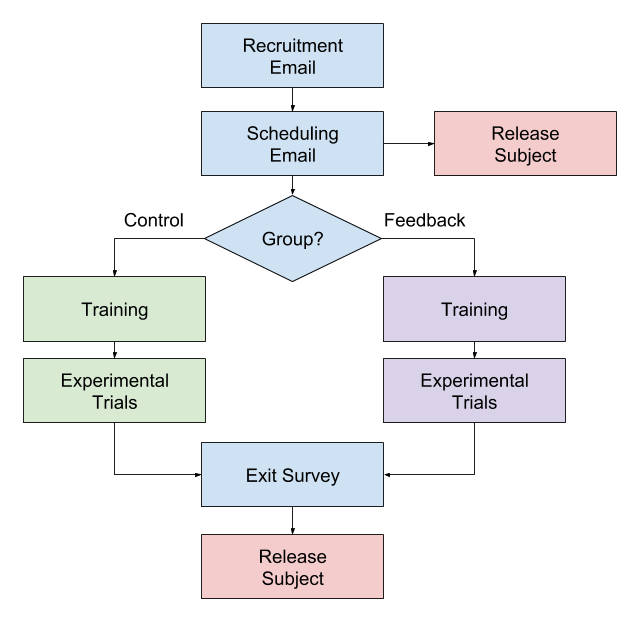
\includegraphics[width=0.75\textwidth]{../img/robot_flow.png}
  \end{center}
\end{frame}

\begin{frame}[fragile]{Experiment Two Estimates}
  \begin{itemize}
    \setlength\itemsep{1em}
    \item 10-15 subjects in each group
    \item 30 minutes of context and training
    \item 1-2 hours of trials
    \item 1-2 months from recruitment to end of subject testing
  \end{itemize}
\end{frame}

\begin{frame}[fragile]{Experiment Two Flowchart}
  \begin{center}
    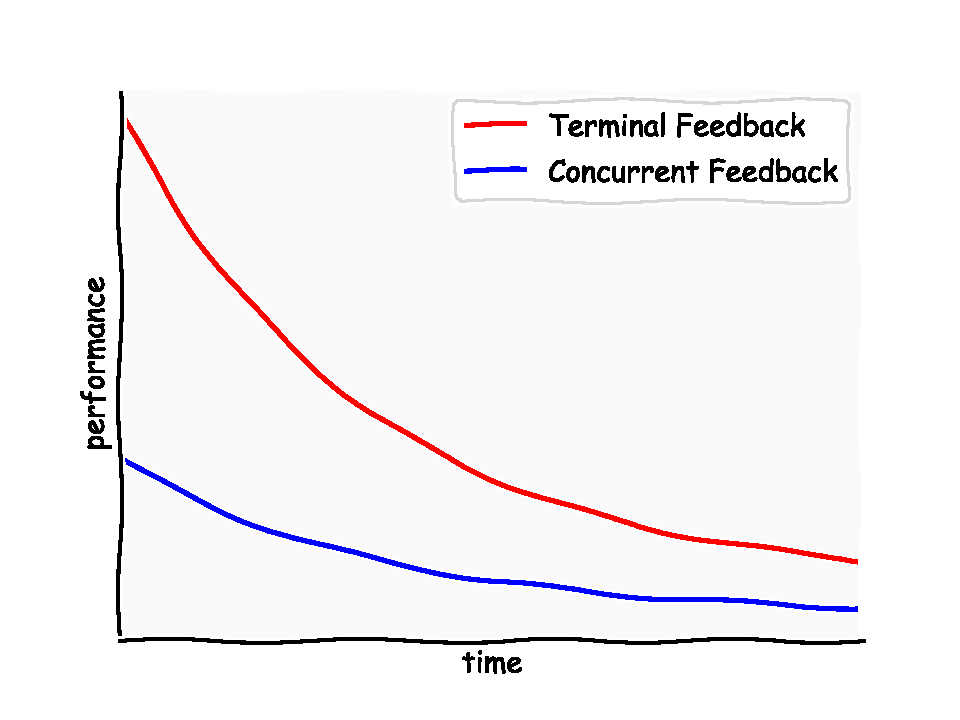
\includegraphics[width=0.75\textwidth]{../img/robot_estimate.pdf}
  \end{center}
\end{frame}

\subsection{Modeling}

\section{Timeline and Risks}

\begin{frame}[fragile]{Timeline}
  \begin{figure}[h!]
    \begin{center}
      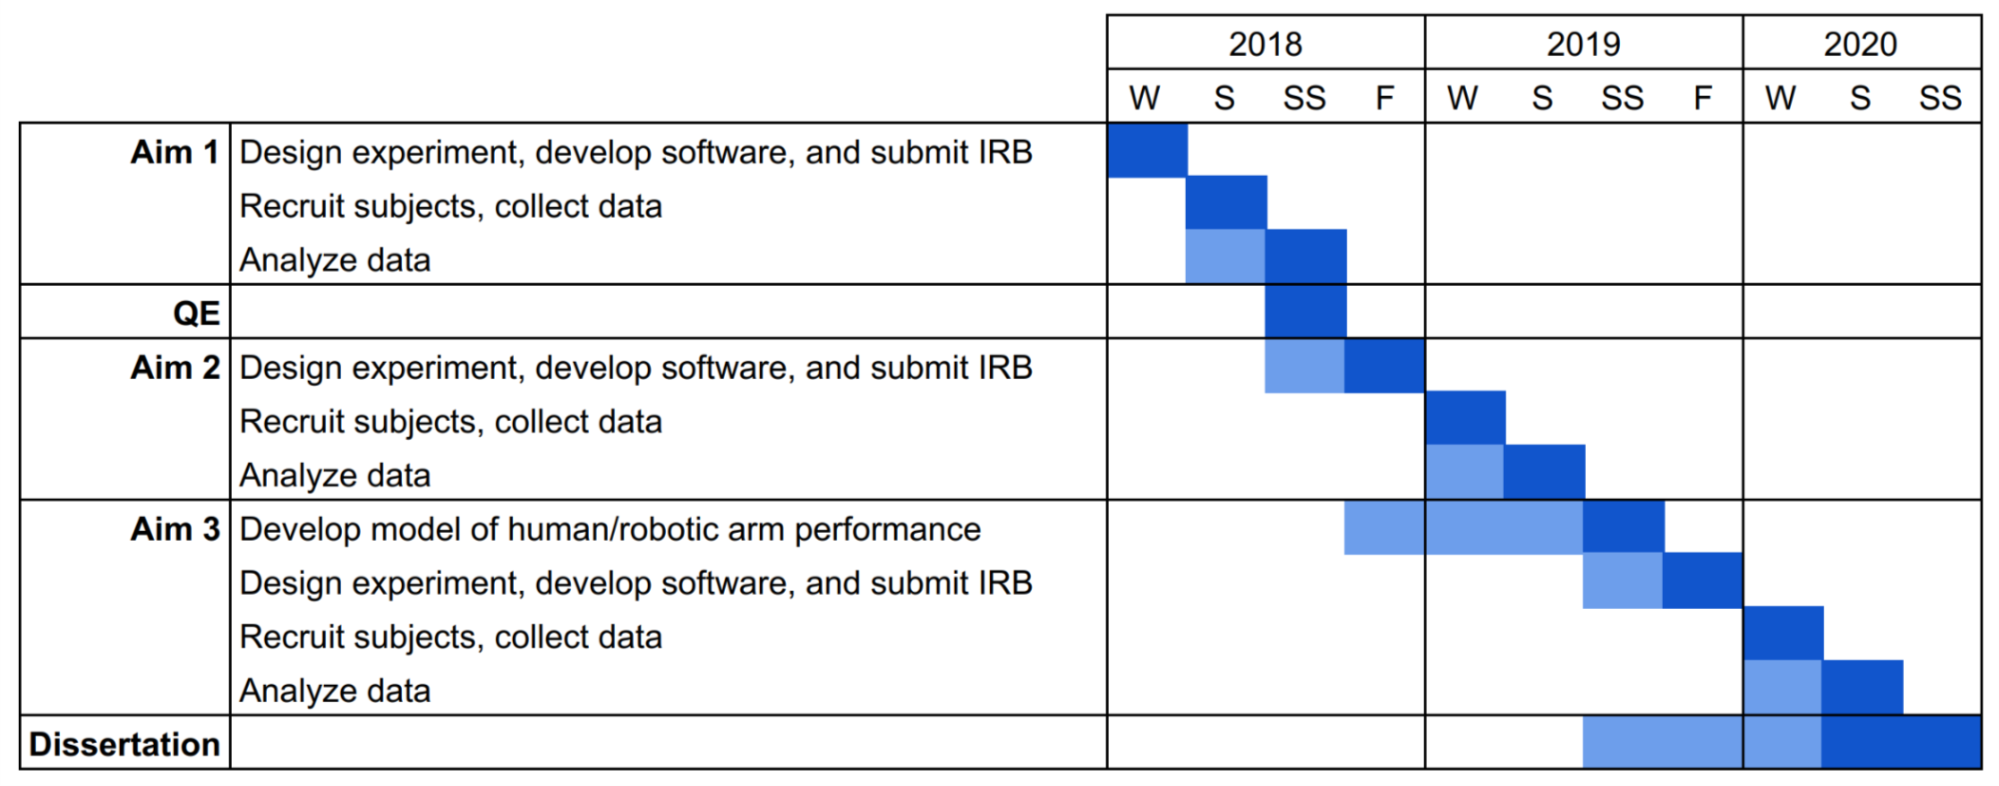
\includegraphics[width=\linewidth]{../img/image1.png}
      % \caption{The proposed timeline for this research.}
      % \label{timeline}
    \end{center}
  \end{figure}
\end{frame}

\begin{frame}[fragile]{Acknowledgments}
  Thank you to
  \begin{itemize}
    \item Link Foundation Modeling, Simulation, and Training Fellowship
    \item Human/Robotics/Vehicle Integration and Performance Lab
    \item NASA Ames Human Systems Integration Division
    \item Qualifying Examination Committee
    \item Professor Robinson
  \end{itemize}
  \hfill
\includegraphics[height=1.5cm]{../img/linkfoundation.png}
\includegraphics[height=1.5cm]{../img/hrvip.png}
\includegraphics[height=1.5cm]{../img/nasa.png}
\end{frame}

\begin{frame}[standout]
  Questions?
\end{frame}

\appendix

% \begin{frame}[fragile]{Backup slides}
%   Sometimes, it is useful to add slides at the end of your presentation to
%   refer to during audience questions.

%   The best way to do this is to include the \verb|appendixnumberbeamer|
%   package in your preamble and call \verb|\appendix| before your backup slides.

%   \themename will automatically turn off slide numbering and progress bars for
%   slides in the appendix.
% \end{frame}


\begin{frame}[allowframebreaks]{References}
  \bibliography{../proposal/bib}
  \bibliographystyle{ieeetr}
\end{frame}

\begin{frame}[fragile]{Performance Analysis by Starting Design}
\begin{figure}
  \begin{center}
    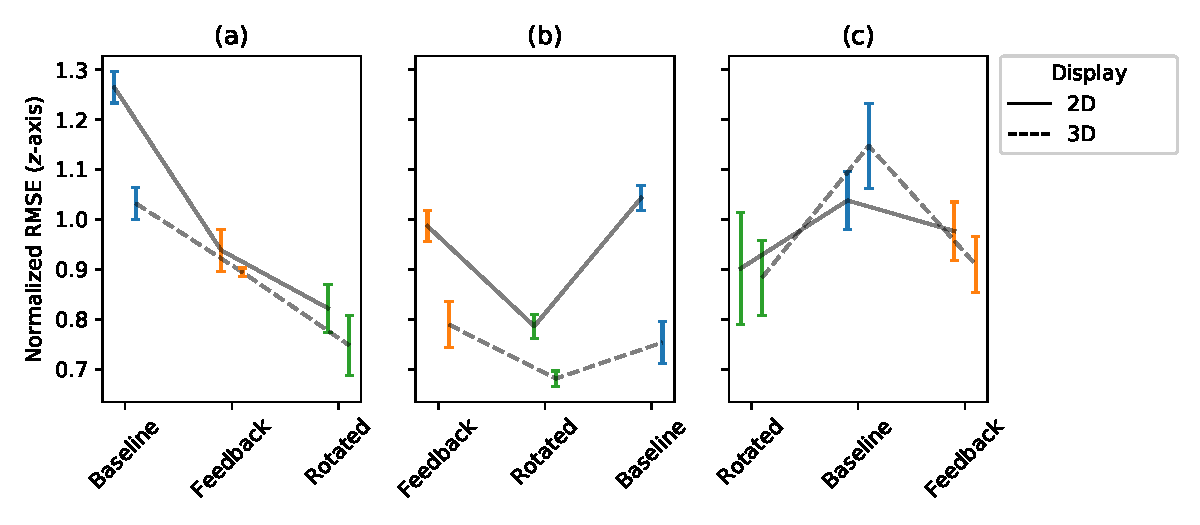
\includegraphics[width=\linewidth]{../img/x_design_y_zrmse_col_startdesign_hue_device.pdf}
  \end{center}
\end{figure}
\end{frame}

\begin{frame}[fragile]{Three-axis tracking rotated design}
  \begin{figure}
    \begin{center}
      \newcommand{\rotateRPY}[3]% roll, pitch, yaw
      {   \pgfmathsetmacro{\rollangle}{#1}
          \pgfmathsetmacro{\pitchangle}{#2}
          \pgfmathsetmacro{\yawangle}{#3}

          % to what vector is the x unit vector transformed, and which 2D vector is this?
          \pgfmathsetmacro{\newxx}{cos(\yawangle)*cos(\pitchangle)}
          \pgfmathsetmacro{\newxy}{sin(\yawangle)*cos(\pitchangle)}
          \pgfmathsetmacro{\newxz}{-sin(\pitchangle)}
          \path (\newxx,\newxy,\newxz);
          \pgfgetlastxy{\nxx}{\nxy};

          % to what vector is the y unit vector transformed, and which 2D vector is this?
          \pgfmathsetmacro{\newyx}{cos(\yawangle)*sin(\pitchangle)*sin(\rollangle)-sin(\yawangle)*cos(\rollangle)}
          \pgfmathsetmacro{\newyy}{sin(\yawangle)*sin(\pitchangle)*sin(\rollangle)+ cos(\yawangle)*cos(\rollangle)}
          \pgfmathsetmacro{\newyz}{cos(\pitchangle)*sin(\rollangle)}
          \path (\newyx,\newyy,\newyz);
          \pgfgetlastxy{\nyx}{\nyy};

          % to what vector is the z unit vector transformed, and which 2D vector is this?
          \pgfmathsetmacro{\newzx}{cos(\yawangle)*sin(\pitchangle)*cos(\rollangle)+ sin(\yawangle)*sin(\rollangle)}
          \pgfmathsetmacro{\newzy}{sin(\yawangle)*sin(\pitchangle)*cos(\rollangle)-cos(\yawangle)*sin(\rollangle)}
          \pgfmathsetmacro{\newzz}{cos(\pitchangle)*cos(\rollangle)}
          \path (\newzx,\newzy,\newzz);
          \pgfgetlastxy{\nzx}{\nzy};
      }

      \tikzset{RPY/.style={x={(\nxx,\nxy)},y={(\nyx,\nyy)},z={(\nzx,\nzy)}}}

      \begin{tikzpicture}
          \draw[-] node at (3.5,0,0) {x} (-3,0,0) -- (3,0,0);
          \draw[-] node at (0,3.5,0) {y, {\color{red} y\textprime}} (0,-3,0) -- (0,3,0);
          \draw[-] node at (0,0,3.5) {z} (0,0,-3) -- (0,0,3);

          \rotateRPY{0}{-30}{0}
          \begin{scope}[draw=red, text=red,fill=red,densely dashed,RPY]
              \draw[-] node at (3.5,0,0) {x\textprime} (-3,0,0) -- (3,0,0);
              %\draw[-] node at (0,3.5,0) {} (0,0,0) -- (0,3,0);
              \draw[-] node at (0,0,3.5) {z\textprime} (0,0,-3) -- (0,0,3);
          \end{scope}
          \draw [->] (0:1.5) arc (0:-15:1.5);
          \draw[-] node at (1.7,-.2,0) {$\theta$};
      \end{tikzpicture}
      % \caption{Perspective display of the coordinate frame for the tracking tasks, with the $x$, $y$, and $z$ axes labeled. After rotating by $\theta$ around the y axis, the resulting reference frame of $x\textprime y\textprime z\textprime$ is also labeled.}
      % \label{designdiagram}
    \end{center}
  \end{figure}
\end{frame}


\end{document}
